\documentclass[
    a4paper,
    fontsize=12pt,
    footinclude=true,
    headinclude=true
	]{scrbook}

	\usepackage{scrhack}
	\usepackage{silence}
	\WarningFilter{latex}{You have requested package}
	\usepackage{template/preamble}
	\setlength{\parskip}{0.3em}

	\renewcommand{\bf}{\normalfont \bfseries}

	\bibliography{biblio.bib}

\usepackage{ifthen}
\usepackage{graphicx}
\usepackage{comment}
\usepackage{amsmath,amssymb} % define this before the line numbering.
\usepackage{color, colortbl}
\usepackage{xcolor}
\usepackage{nicefrac}
\usepackage{booktabs}
\usepackage{placeins}
\usepackage{pifont}
\usepackage{subcaption}
\usepackage{xspace}
\usepackage{arydshln}
\usepackage{nicefrac}

\newcommand{\titlecaption}[3][]{\caption[#2]{\textbf{#2}\ifthenelse{\equal{#1}{}}{. }{ }#3}}

\newcommand{\todo}[1]{\textcolor{BrickRed}{[TODO #1]}}
\newcommand{\note}[1]{\textcolor{PineGreen}{(#1)}}
\newcommand{\review}[1]{\textcolor{RoyalBlue}{#1}}
\newcommand{\startreview}{\color{RoyalBlue}}
\newcommand{\stopreview}{\color{black}}
\definecolor{yellowdark}{HTML}{BC8C00}
\definecolor{bluedark}{HTML}{2F528F}
\definecolor{greendark}{HTML}{507E32}
\definecolor{bluefig}{HTML}{5B9BD5}

\definecolor{lightblueborder}{HTML}{41719C}
\definecolor{lightbluefill}{HTML}{5E9CD3}

\let\oldleftmark=\leftmark


\newboolean{skipIntro}
\newboolean{skipRelated}
\newboolean{skipRegul}
\newboolean{skipSegm}
\newboolean{skipDyna}
\newboolean{skipRepet}
\newboolean{skipConclusion}
\newboolean{skipAppendix}

\setboolean{skipIntro}{false}
\setboolean{skipRelated}{true}
\setboolean{skipRegul}{false}
\setboolean{skipSegm}{true}
\setboolean{skipDyna}{true}
\setboolean{skipRepet}{true}
\setboolean{skipConclusion}{true}
\setboolean{skipAppendix}{true}
% By setting this to true, you skip the compiling of some chapters
% \setboolean{skipIntro}{true}
% \setboolean{skipSHADE}{true}
% \setboolean{skipHN}{true}
% \setboolean{skipDual}{true}

%\mtcsetoffset{minitoc}{-0.80em}
\setlength{\mtcindent}{-0.80em}

\newcommand{\cmark}{\ding{51}}%
\newcommand{\xmark}{\ding{55}}%


\begin{document}

\dominitoc
\selectlanguage{english}

\frontmatter

\begin{titlepage}

  \vspace*{-2.5cm}
  
\includegraphics[height=0.15\columnwidth]{images/sorbonne}
  \hspace*{2.5cm}
  
\includegraphics[height=0.15\columnwidth]{images/heuritech}
  \vspace*{0.5cm}

  \begin{center}

    {\large \textbf{T\normalsize{HÈSE DE}\large{} D\normalsize{OCTORAT DE}\large{} S\normalsize{ORBONNE}\large{} U\normalsize{NIVERSITÉ}}}\\
    Spécialité \textbf{Informatique}\\
    École Doctorale Informatique, Télécommunications et Électronique (Paris)

    \vspace*{1.5cm}

    {\Large \textbf{Continual Learning models for Computer Vision}} \\[0.5em]
    {\large \textbf{Apprentissage Continu pour la Vision par Ordinateur}}

    \vspace*{1.2cm}

    Présentée par\\
    {\large \textbf{Arthur {Douillard}}}

    \vspace*{2mm}

    Dirigée par\\
    \textbf{Pr. Matthieu {CORD}}

    \vspace*{5mm}

    Pour obtenir le grade de \ \\
    \textbf{DOCTEUR de SORBONNE UNIVERSITÉ} \ \\

    \vspace*{5mm}

  \end{center}

  \definecolor{mygray}{gray}{0.37}
  \newcommand{\affil}[1]{\multicolumn{2}{@{\hskip 18pt}l@{}}{\small \itshape \textcolor{mygray}{#1}}}

  %\vspace*{5mm}
  \flushleft{
    Présentée et soutenue publiquement le 13 juin 2022\\[2mm]
    Devant le jury composé de :\\[2mm]
    \begin{tabularx}{\textwidth}{@{\hskip 18pt}Xr}
      Dr. Diane \textsc{Larlus} & Rapportrice       \\[-0.5mm]
      \affil{Research Scientist, Naver Labs Europe} \\[0.5mm]
    \end{tabularx}
    \begin{tabularx}{\textwidth}{@{\hskip 18pt}Xr}
      Pr. David \textsc{Filliat} & Rapporteur \\[-0.5mm]
      \affil{Professor, INRIA/ENSTA Paris}    \\[0.5mm]
    \end{tabularx}
    \begin{tabularx}{\textwidth}{@{\hskip 18pt}Xr}
      Pr. Tatiana \textsc{Tommasi} & Examinatrice        \\[-0.5mm]
      \affil{Associate Professor, Politecnico di Torino} \\[0.5mm]
    \end{tabularx}
    \begin{tabularx}{\textwidth}{@{\hskip 18pt}Xr}
      Dr. Karteek \textsc{Alahari} & Examinateur \\[-0.5mm]
      \affil{Research Scientist, INRIA Grenoble} \\[0.5mm]
    \end{tabularx}
    \begin{tabularx}{\textwidth}{@{\hskip 18pt}Xr}
      Pr. Kévin \textsc{Bailly} & Examinateur \\[-0.5mm]
      \affil{Associate Professor, Sorbonne}   \\[0.5mm]
    \end{tabularx}
    \begin{tabularx}{\textwidth}{@{\hskip 18pt}Xr}
      Pr. Matthieu \textsc{Cord} & Directeur de thèse \\[-0.5mm]
      \affil{Professor, Sorbonne }                    \\[0.5mm]
    \end{tabularx}
    \begin{tabularx}{\textwidth}{@{\hskip 18pt}Xr}
      Dr. Thomas \textsc{Robert} & Invité \\[-0.5mm]
      \affil{Head of Research, Heuritech} \\[0.5mm]
    \end{tabularx}

  }
  %}

\end{titlepage}
\thispagestyle{empty}

\hfill

\vfill

\noindent\myName: \textit{\myTitle,}
\textcopyright\ 2022


% TOC

% \acused{AE}
% \acused{SHADE}
% \acused{SWWAE}
% \acused{HySWWAE}
\microtypesetup{protrusion=false}
\cleardoublepage
\addcontentsline{toc}{chapter}{\texorpdfstring{\noexpand\spacedlowsmallcaps{\contentsname}}{\contentsname}}
\setcounter{tocdepth}{1}
\setcounter{minitocdepth}{2}
\setcounter{secnumdepth}{3}
\manualmark
\markboth{\spacedlowsmallcaps{\contentsname}}{\spacedlowsmallcaps{\contentsname}}
\tableofcontents
\adjustmtc
\automark[section]{chapter}
\renewcommand{\chaptermark}[1]{\markboth{\spacedlowsmallcaps{#1}}{\spacedlowsmallcaps{#1}}}
\renewcommand{\sectionmark}[1]{\markright{\thesection\enspace\spacedlowsmallcaps{#1}}}
\microtypesetup{protrusion=true}

\cleardoublepage
\addcontentsline{toc}{chapter}{\texorpdfstring{\noexpand\spacedlowsmallcaps{\listfigurename}}{\listfigurename}}
\listoffigures
\adjustmtc

\cleardoublepage
\addcontentsline{toc}{chapter}{\texorpdfstring{\noexpand\spacedlowsmallcaps{\listtablename}}{\listtablename}}
\listoftables
\adjustmtc

\cleardoublepage
\setcounter{page}{1}

\chapter{Abstract}

I first review the existing methods based on regularization for continual learning. While
regularizing a model's probabilities is very efficient to reduce forgetting in large-scale datasets,
there are few works considering constraints on intermediate features. I cover in this chapter two
contributions aiming to regularize directly the latent space of \acs{ConvNet}. The first one,
PODNet, aims to reduce the drift of spatial statistics between the old and new model, which in
effect reduces drastically forgetting of old classes while enabling efficient learning of new
classes. I show in a second part a complementary method where we avoid pre-emptively forgetting by
allocating locations in the latent space for yet unseen future class.

Then, I describe a recent application of \acf{CIL} to semantic segmentation. I show that
the very nature of \acf{CSS} offer new specific challenges, namely forgetting on large
images and a background shift. We tackle the first problem by extending our distillation
loss introduced in the previous chapter to multi-scales. The second problem is solved by
an efficient pseudo-labeling strategy. Finally, we consider the common rehearsal learning,
but applied this time to \ac{CSS}. I show that it cannot be used naively because of memory
complexity and design a light-weight rehearsal that is even more efficient.

Finally, I consider a completely different approach to continual learning: dynamic networks
where the parameters are extended during training to adapt to new tasks. Previous works on
this domain are hard to train and often suffer from parameter count explosion. For the
first time in continual computer vision, we propose to use the Transformer architecture:
the model dimension mostly fixed and shared across tasks, except for an
expansion of learned task tokens. With an encoder/decoder strategy where the decoder
forward is specialized by a task token, we show state-of-the-art robustness to forgetting
while our memory and computational complexities barely grow.


\cleardoublepage


\chapter{R\'esum\'e}

\selectlanguage{french}

Depuis le début des années 2010 la recherche en apprentissage automatique a orienté son attention
vers les efficaces réseaux de neurones profonds. Plus particulièrement, toutes les tâches de vision
par ordinateur utilisent désormais des réseaux convolutionnels. Ces modèles apprennent à détecter
des motifs d'abord simples (contours, textures) puis de plus en plus complexes jusqu'à apprendre
le concept d'objets en particulier.

Malgré les grandes avancées dans le domaine des réseaux de neurones profonds, un problème important
subsiste : comment apprendre une quantité croissante de concepts, à la manière d'un élève durant sa
scolarité, sans oublier les précédentes connaissances. Ce problème d'apprentissage continu est
complexe : si non traité, les réseaux de neurones oublient catastrophiquement. L'objectif de cette
thèse était donc de résoudre de ce problème.

J'ai pu dans un premier temps développer plusieurs méthodes pour forcer un comportement similaire
entre la version du modèle ayant appris de nouveaux concepts et sa précédente itération.
Contrairement au reste de la littérature, qui imposait des contraintes sur le comportement final du
modèle, je me suis intéressé aux représentations internes.

Dans un second temps, j'ai considéré l'apprentissage continu pour la tâche de segmentation
sémantique. Cette tâche complexe possède des problèmes inédits dans un contexte continu en plus de
l'oubli catastrophique. J'ai pu proposer plusieurs approches complémentaires pour les résoudre. Plus
précisément : une nouvelle méthode de contraintes, une technique de pseudo-annotations et une
manière efficace de révisions d'objets.

Et enfin, dans un troisième et dernier temps, je m'intéresse aux réseaux de neurones dynamiques,
pouvant créer de nouveaux neurones à travers leur existence pour résoudre un nombre croissant de
tâche. Les méthodes précédentes grandissent avec peu de contrôles, résultant en des modèles
extrêmement lourd, et souvent aussi lents. Donc, en m'inspirant des récents \textit{transformers},
j'ai conçu une stratégie dynamique avec un coût pratiquement nul, mais ayant malgré tout des
performances à l'état-de-l'art.

\selectlanguage{english}

\cleardoublepage
\chapter{Remerciements}

\selectlanguage{french}

Je souhaite remercier tous ceux qui m'ont aidé à réaliser cette thèse.

Dans un premier temps, je dois Charles Ollion, et Tony Pinville: Matthieu pour m'avoir supervisé tout
au long de ces trois années de thèse, pour m'avoir fait découvrir le monde de la recherche et avoir
supporté mes avis tétus. J'ai beaucoup appris et j'en ressors grandis. Charles et Tony pour m'avoir
fait confiance et permis de faire ce doctorat avec Heuritech. Et plus particulièrement Charles, pour
avoir été le premier à m'initier au Deep Learning.

Je remercie aussi le jury de cette thèse pour avoir relu mon manuscrit et être m'accorder leur temps
pour ma soutenance.

Je veux aussi remercier tous mes collègues dont leur discussions ont toujours été enrichissante
aussi bien sur le plan du travail que de l'humain. Parmi les \textit{Chordettes}: Corentin Dancette,
Rémi Cadene, Alexandre Ramé, Antoine Saporta, Guillaume Couairon, Asya Grechka, Yifu Chen et Rémy
Sun. Chez Heuritech: Thomas Robert (pour sa gentillesse infinie), Emilien Garreau, Antoine
Hoorelbeke, Paul Morel, Florent Mercier, et Oscar Bouvier. Et enfin aussi Timothée Lesort, Fabio
Cermelli, Eduardo Valle et Arnaud Dapogny pour leur collaboration. Plus largement je remercie aussi
l'ensemble de l'équipe du MLIA et Heuritech pour leur support et la bonne ambiance qu'ils ont
apporté.

Enfin, je veux remercier mes proches. A Jordan et Camille qui m'ont tant soutenu cette dernière
année. A David, Hugo, Alexandre, Thibault et Marie-Anne, Benjamin, Florent, Sarasvati, Charlotte, et
tous ceux avec qui j'ai pu passer de bons moments. A ma famille, Julie, mon père, ma mère, mes
grand-parents pour leur soutien durant ces 26 ans de vie. J'insiste particulièrement sur l'éducation
et la passion des sciences que m'ont inculqués ma mère et ma grand-mère, qui a été essentiel.


\selectlanguage{english}


\cleardoublepage
% \faketableofcontents
\chapter{Acronyms}

\begin{acronym}[XXXXXXX]
    \acro{AI}{Artificial Intelligence}
    \acro{BN}{Batch Normalization}
    \acro{ConvNet}[\textlarger{ConvNet}]{Convolutional Neural Network}
    \acro{CV}{Computer Vision}
    \acro{DA}{Data Augmentation}
    \acro{FC}{Fully Connected}
    \acro{DL}{Deep Learning}
    \acro{DNN}{Deep Neural Network}
    \acro{GAN}{Generative Adversarial Network}
    \acro{GPU}{Graphics Processing Unit}
    \acro{ML}{Machine Learning}
    \acro{MLP}{Multi-Layer Perceptron}
    \acro{MSE}{Mean-Squared Error}
    \acro{NN}{Neural Network}
    \acro{ReLU}{Rectified Linear Unit}
    \acro{SGD}{Stochastic Gradient Descent}
    \acro{SIFT}{Scale-Invariant Feature Transform}
    \acro{SSL}{Semi-Supervi\-sed Learning}
    \acro{TPU}{Tensor Processing Unit}
    \acro{LSC}{Local Similarity Classifier}
    \acro{POD}{Pooled Output Distillation}
    \acro{PODNet}{Pooled Output Distillation Network}
    \acro{PLOP}{Pseudo-labeling and LOcal Pod}
    \acro{DyTox}{Dynamic Token Expansion}
    \acro{NC}{New Classes}
    \acro{NI}{New Instances}
    \acro{NIC}{New Instances and Classes}
    \acro{CIL}{Class Incremental Learning}
    \acro{CL}{Continual Learning}
    \acro{ZSL}{ZeroShot-Learning}
    \acro{KL}{Kullback-Leiber divergence}
    \acro{KD}{Knowledge Distillation}
    \acro{NME}{Nearest Mean Examplar}
    \acro{SVM}{Support-Vectors Machine}
    \acro{CSS}{Continual Semantic Segmentation}
    \acro{CNN}{Convolutional Neural Network}
    \acro{NLP}{Natural Language Processing}
    \acro{NN}{Neural Network}
    \acro{NC}{New Classes}
    \acro{NI}{New Instances}
    \acro{NIC}{New Instances and Classes}
    \acro{AL}{Active Learning}
    \acro{KD}{Knowledge Distillation}
    \acro{GAP}{Global Average Pooling}
\end{acronym}


\mainmatter

\chapter{Introduction}
\label{chapter:introduction}

%\minitoc
\chapterwithfigures{\nameref*{chapter:introduction}}
%\chapterwithtables{\nameref*{chapter:introduction}}

\ifthenelse{\boolean{skipIntro}}{\endinput}{}


% what is ai
% application of ai
% ethical limits

% computer vision, input/output
% M/D Learning, abstract, no math
% heuritech
% continual learning what are the problems
% outline, maybe fusionned with CL

\epigraph{I believe that at the end of the century, the use of words and general educated opinion
      will have altered so much that one will be able to speak of machines thinking without expecting to
      be contradicted.}{\textit{Alan Turing}}

In this thesis introduction, using layman terms, I describe Artificial Intelligence, and,
in particular, one of its instances: Deep Learning. Then, I lay out the challenges of this
thesis and what I have developed to solve them.

%\section{Artificial Intelligence}

\textbf{The idea of thinking machines} began in the previous century, from Karel Çapek's invention of the
"\textit{robot}" to the 1956's Dartmouth workshop passing by Turing \& von Neumann's reflections.
Despite suffering from multiple "AI winters" filled with disappointments and criticisms, Turing's
prediction on the rising importance of \ac{AI} proved to be right as the first and the second
decades of the XXI century saw the advent of respectively \acf{ML} and \acf{DL}, two major subfields
of \ac{AI}.

Providing \textbf{a definition of \ac{AI}} is difficult, but its foremost domains, \ac{ML} and \ac{DL}, can be
defined as statistical methods aiming to discover patterns in data. These methods are already
ubiquitous: speech recognition enabling us to control devices remotely, recommender
systems proposing movies according to our taste, automatic translation, face recognition,
autonomous driving, \etc. Less known but still useful applications comprise accelerated physics
simulation, protein folding prediction, molecule toxicity estimation, data center cooling system, and
control of the magnetic coils of a nuclear fusion reactor.

\ac{AI} is increasingly more important in our daily lives with some applications raising \textbf{ethical
      concerns}: face recognition biased towards some populations, loan grants, medical diagnosis, justice
advice, chatbots with toxic behavior, \etc. Therefore, we must pay a particular interest on the
potential impact of this new technology. Towards this goal, a diverse set of profiles, in all steps
of a product, must be trained to recognize these issues.

\section{Deep Learning}

While many domains exist in \acf{AI}, this thesis is focused on using \acf{DL} applied to \acf{CV}.
In this section, I will briefly describe the learning methods and the data structure.
Finally, I will detail the challenges tackled in this thesis and why they matter.

\paragraph{Deep Learning} belongs to the statistical learning methods. As other statistical methods,
such as \acf{ML}, these methods usually work on an input/output level. Given an input, the model
produces an output called \textit{prediction}. Then, it is compared to what the model should
predict, \ie the \textit{ground-truth}. Like in human learning, the model is informed when it is
wrong to avoid making the same mistake twice. \acf{DL} models are based on artificial neural
networks, and as the name implies, which bear some similarity with humans' neurons.

\paragraph{Computer Vision} is an application topic in \acf{AI}. Its goal is to analyze images using
a computer-assisted method. The most common tasks in \acf{CV} includes image classification where a
label must be predicted per image, semantic segmentation where each pixel must be attributed a label
or even \ac{VQA} where questions about an image must be answered. Several families of methods can be
used to tackle \ac{CV} problems, but as of 2012 and onwards, \acf{DL} is the best performing method
for this type of data.

\section{This Thesis}

Now with the type of methods and data (Deep Learning and images) defined, I will contextualize my
thesis w.r.t. my sponsor, how it influenced my research, and what challenges I have aimed to tackle.

\paragraph{Heuritech} This thesis was sponsored by the Parisian startup
Heuritech\footnote{\url{https://heuritech.com}} as a \textit{CIFRE PhD}. The company analyzes social
networks such as Instagram and Weibo, recognizes the clothes in pictures, estimates
volumes of fine-grained types of garments, and finally forecasts future trends. The company's
\acf{CV} models must recognize an ever-growing number of entities from features (\eg knitted, blue
color, short cut) to brand models (\eg Nike Air Max, Adidas Stan Smith, Puma Suede). This
requirement leads to two problems: \textbf{(1)} the time spent to re-train a model is growing
linearly, and \textbf{(2)} learning a new entity can incur a performance loss on previously learned
entities. The scientific literature names the domain of learning new concepts incrementally
``\textbf{Continual Learning}'', and the loss of performance ``\textbf{Catastrophic Forgetting}''.

\paragraph{Continual Learning} is a field that emerged in the 1990s but saw renewed interest only
very recently around the second half of the 2010s. The goal is to deal with non-static datasets that
evolve through time. This evolution can take many forms, including adding new entities to predict in
a classification task (\eg learning sneaker brands, then high-heel brands) or adding samples from
new sources (\eg commercial photoshoot then images from social media). Unfortunately, current
State-of-the-Art models struggle to learn continually without forgetting. This loss is so critical
that the literature nicknamed it a ``catastrophic forgetting''. Multiple methods have been designed
to reduce this forgetting; the two major ones being rehearsal and constraints. Rehearsal involves
reviewing previously learned knowledge, as a human student would \textit{rehearse} the last
semester's course. However, this rehearsal is often limited in order to reduce computational cost
and because past data may not always be available for a variety of reasons, including privacy. On
the other hand, constraints enforce the model to keep a similar \textit{behavior} as it learns new
concepts, but defining the right constraint is not trivial.

\paragraph{Thesis's Outline:} This thesis is focused on bringing Continual Learning capacity to
Computer Vision models. In the next chapter (\autoref{chapter:related}), I detail the learning
procedure, state the exact benchmarks considered in Continual Learning, and review the
State-of-the-Art methods in this domain. Then, I cover the work I have done during this thesis over
three chapters as follows:

\begin{itemize}
      \item \autoref{chapter:regularization}: \nameref{chapter:regularization}\\
            I first review the existing methods based on regularization for continual learning. While
            regularizing a model's probabilities is very efficient to reduce forgetting in large-scale
            datasets, there are few works considering constraints on intermediate features. I cover in this
            chapter two contributions aiming to regularize the latent space of \acs{ConvNet} directly. The
            first one, \acf{PODNet} aims to reduce the drift of spatial statistics between the old and new
            model, which in effect reduces drastically forgetting even on an important amount of tasks. I show in a
            second part a complementary method where we avoid pre-emptively forgetting by allocating
            locations in the latent space for yet unseen future class.
      \item \autoref{chapter:segmentation}: \nameref{chapter:segmentation}\\
            Then, I describe a recent application of \acf{CIL} to semantic segmentation. I show that
            the very nature of \acf{CSS} offers new specific challenges, namely forgetting on large
            images and a background shift. We tackle the first problem by extending our distillation
            loss introduced in the previous chapter to multi-scales. The second problem is solved by
            our efficient pseudo-labeling strategy. Finally, we consider the common rehearsal learning
            but applied this time to \ac{CSS}. I show that it cannot be used naively because of memory
            complexity and design a memory-efficient rehearsal that is even more efficient.
      \item \autoref{chapter:dynamic}: \nameref{chapter:dynamic}\\
            Finally, I consider a completely different approach to continual learning: dynamic networks
            where the parameters are extended during training to adapt to new tasks. Previous works on
            this domain are hard to train and often suffer from parameter count explosion. For the
            first time in continual computer vision, we propose to use the Transformer architecture:
            the model's parameters are shared across tasks except for an
            expansion of learned task tokens. With an encoder/decoder strategy where a task token
            specializes the decoder's forward, we show state-of-the-art robustness to forgetting
            while our memory and computational complexities barely grow.
\end{itemize}

\paragraph{Related Publications:} This thesis is based on the materials published in the following papers:

\begin{itemize}
      \item \fullcite{douillard2020podnet}
      \item \fullcite{douillard2020ghost}
      \item \fullcite{douillard2020plop}
      \item \fullcite{douillard2021objectrehearsal}
      \item \fullcite{douillard2021dytox}
\end{itemize}

I have also published other papers that can be found in the \autoref{chapter:appendix}:

\begin{itemize}
      \item \fullcite{douillardlesort2021continuum}
      \item \todo{Add ICML submission on foundation models with MILA}
      \item \todo{Add CTKT with Antoine}
\end{itemize}


\cleardoublepage

\acresetall
\chapter{Related Works}
\label{chapter:related}

%\begin{chapabstract}
%      Deep Learning is now the major method to learn unstructured data such as images. Computer
%      Vision used for a long time handcrafted convolution kernels, but nowadays, they are learned:
%      each value of the kernel is a neuron. This kind of network, called \acf{CNN}, showed
%      impressive performance in a wide variety of tasks. However, they still suffer from the plague
%      of forgetting when learning a moving distribution as new samples, from new sources or new
%      classes appear. Continual Learning aims to solve this challenge using multiple
%      approaches, including rehearsal and behavior constraints.
%\end{chapabstract}

%\minitoc
\chapterwithfigures{\nameref*{chapter:related}}
\chapterwithtables{\nameref*{chapter:related}}

\ifthenelse{\boolean{skipRelated}}{\endinput}{}


In this chapter, we detail the related work needed to read this thesis. We first briefly
explain the learning procedure in \acf{DL} and how the data are structured. Then, we describe how
\ac{DL} applications and architectures in \acf{CV}. Finally, we introduce the main topic of this thesis
---Continual Learning--- and showcase the challenges, benchmarks, and methods of this domain. The
notations introduced in this chapter and thorough the thesis are listed in the
\hyperref[chap:notations]{Notations}.

\section{Neural Network Learning}

Neural Networks are based on the statistical learning theory \citep{vapnik1999statstheory}. In the
\textit{supervised setting}, the goal of a neural network is to learn the best mapping function $f :
      \mathcal{X} \rightarrow \mathcal{Y}$ between an input space $\mathcal{X}$ and an output space
$\mathcal{Y}$.  We consider a \textit{loss} function $\mcL : \mathcal{Y} \times \mathcal{Y} \rightarrow
      \mathbb{R}^+$ that measures the disagreement between a ground-truth label $y$ and the network's
prediction $\hat{\vy} = f(\vx)$. In the context of image classification, the $\vx$ is the image
pixels, $y$ is the \textit{class} label of the object present in the image, and $\hat{\vy}$ is a
vector of probabilities, with one probability per class the model has to predict. The highest class
with the highest predicted probability/confidence is chosen as the prediction.
Given a \textit{training dataset} $\mathbb{D} = \{(\vx_1, y_1), ..., (\vx_N, y_N)\}$, training a neural network
consists in finding the set of parameters $\theta^*$ which minimizes the loss function:
%
\begin{equation}
      \theta^* = \operatorname{argmin}_{\theta} \left \{ \mathbb{E}_{(\vx,y) \sim \mathbb{D}} \mcL(f_\theta(\vx, y))\right \}\,.
      \label{eq:intro_optim}
\end{equation}
%
However, the optimal set of parameters $\theta^*$ minimizing the loss on the training set, can fail
to predict the correct label on the testing set. Therefore, to avoid this \textit{overfitting} phenomenom,
regularization functions that limit the parameters space are used as additional constraints in addition
to the classification loss $\mcL$.

In practice, the function $f_\theta$ learned by a neural network is composed of a succession of linear
transformations and non-linear \textit{activation} functions. For example, a simple neural network,
called \ac{MLP} could be defined as:
%
\begin{equation}
      \hat{\vy} = f_\theta(\vx) = \operatorname{softmax}(\vW_o \sigma(\vW_h \vx + \vb_h) + \vb_o))\,,
      \label{eq:intro_mlp}
\end{equation}
%
\noindent with $\vW_h \in \mathbb{R}^{H \times D}$, $\vb_h \in \mathbb{R}^{H}$, $\vW_o \in
      \mathbb{R}^{C \times H}$, $\vb_o \in \mathbb{R}^{C}$ being the parameters $\theta$ of the
network. $\sigma$ is a hidden non-linear activation, often a \ac{ReLU}
($\operatorname{ReLU(x)} = \text{max}(0, x)$), and $\operatorname{softmax}(\tilde{\vy}) =
      \nicefrac{e^{\tilde{\vy}}}{\sum_{i} e^{\tilde{\vy}_i}}$ is the final non-linear activation.

Likewise, in practice for image classification, the loss is often the categorical cross-entropy:
%
\begin{equation}
      \mcL(\hat{\vy}, \vy) = -\sum_i y_i \log \hat{y}_i\,,
      \label{eq:intro_ce}
\end{equation}
%
\noindent with $\vy$ a one-hot vector of the labels. Finally, to optimize the parameters of the neural
network (such as \autoref{eq:intro_optim}), we often use the mini-batch \ac{SGD} algorithm or a variation thereof:

\begin{algorithm}
      \begin{algorithmic}[1]
            \Statex \textbf{input:} a dataset $\mathbb{D}$ with pairs of $(\vx, \vy)$
            \Statex \textbf{input:} a loss function $\mcL$
            \Statex \textbf{input:} a model function $f_\theta$ with $\theta$ the learned parameters
            \Statex \textbf{input:} a learning rate $\eta$ and a batch size $b$
            \Statex

            \While{stopping criterion not satisfied}
            \State $\vx$, $\vy$ $\gets$ sample mini-batch of size $b$ from $\mathbb{D}$
            \State Forward pass: $\hat{\vy}$ $\gets$ $f_\theta(\vx)$
            \State Compute loss: $\mcL$ $\gets$ $\mcL(\hat{\vy}, \vy)$
            \State Compute the gradients: $\delta$ $\gets$ $\nabla_\theta \mcL$
            \State Update all parameters: $\theta$ $\gets$ $\theta - \eta \delta$
            \EndWhile
      \end{algorithmic}
      \caption{Procedure to optimize a neural network with gradient descent.}
      \label{algo:intro_sgd}
\end{algorithm}

The learning rate $\eta$ controls the step size when updating the parameters in the direction of the
gradient. The batch size $b$ defines the number of images seen during one update.
\textit{backpropagation} algorithm computes the gradients and the update of the parameters. In the case
of image classification, the main topic explored in this thesis, we discern the \textit{feature extractor}
from the \textit{classifier} in the neural network. The former transforms the input space so that the latter
linearly discriminates classes. From now on, the feature extractor will be denoted by $f$, and the classifier
by $g$ (more information in the \hyperref[chap:notations]{notations}).

The neural network in \autoref{eq:intro_mlp} can be defined as \textit{shallow} with only one hidden layer.
By extension, an important success of later neural networks came with training \textit{deep} neural
network with multiple hidden layers. More generall
y in this thesis, we will refer to them as \acf{DL}
models.
The majority of \ac{DL} models, in \acf{CV}, in \acf{NLP}, or even in Audio are based on the same structure
(linear transformations and non-linear activations) and are trained with a form of gradient descent.

\section{Deep Architectures for Computer Vision}

A common type of architectures for computer vision is the \acf{ConvNet}. First defined by
\cite{fukushima1980neocognitron} and then trained with backpropagation by \cite{lecun1999lenet}, it
is a neural network architecture whose linear transformations are \textit{convolutions}. While
handcrafted convolutions \citep{lowe1999sift} rely on well-defined features, \ac{ConvNet} can learn
the convolution kernels to detect more complex patterns in order to minimize the classification
loss. In 2012, thanks to a large dataset and more efficient code working on \acp{GPU},
\cite{krizhevsky2012alexnet} won the ILSVC competition \citep{russakovsky2015imagenet_ilsvrc} where
they had to classify a large dataset ---ImageNet--- made of 1M2 training images and 1000 classes.
From that point forward, multiple improvements were made to \ac{ConvNet}
\citep{ioffe2015batchnorm,he2016resnet} and these methods have been applied not only to
classification but also object detection \citep{ren20fasterrcnn}, semantic segmentation
\citep{chen2018deeplab}, visual question answering \citep{antol2015vqa}, \etc.

Most \acp{ConvNet} follow a similar structure with blocks of convolutions and pooling. Usually, the
final spatial features are flattened by \ac{GAP} and fed to a linear classifier
predicting the classes probabilities. \autoref{fig:related_cnn} illustrates this general paradigm.

\begin{figure}[tb]
      \begin{center}
            \includegraphics[width=\linewidth]{images/related/cnn.pdf}
      \end{center}
      \caption{\textbf{A Convolutional Neural Networks} extracts more complex patterns through its
            succession of convolutions. In \textcolor{orange}{orange} a convolution, in \textcolor{red}{red}
            a pooling, and in \textcolor{green}{green} the classifier. Given an image, the \ac{CNN} can assign to
            each possible class a probability, all summing to 1.
            Detected patterns taken from \cite{olah2017feature}.}
      \label{fig:related_cnn}
\end{figure}

\paragraph{Architectures:}The 2010's decade saw major improvements to \acp{CNN}, both in their
architecture structure and in their training procedure. \cite{srivastava2015highwaynet} and
\cite{he2016resnet} propose residual connections between blocks likewise: $\vy = \vx +
      \sigma(\operatorname{Conv}(\vx))$. By reducing the \textit{vanishing gradient} problem
\citep{hochreiter2001vanishinggrad}, it allows training deeper networks without accuracy
degradation. This type of connection is now quasi-ubiquitous in all \ac{DL} based architectures.
Other architecture changes include using convolutions of different kernel sizes in parallel as in
Inception \citep{szegedy2015inception}, enabling a multi-scales view of the features. These
architectures are depicted in \autoref{fig:related_resnet_inception}.

\begin{figure}[tb]
      \begin{center}
            \includegraphics[width=\linewidth]{images/related/resnet_inception.pdf}
      \end{center}
      \caption{\textbf{Different CNN architectures:} \textbf{(a)} illustrates a ResNet-like
            architecture where there are residual connections between blocks. Used by the vast
            majority of modern architectures, these connections reduce the vanishing gradient problem
            and thus enabling the training of deeper networks. \textbf{(b)} showcases an Inception-like
            architecture where at the same level convolutions with different kernel sizes are used.
            Each detects patterns of different scales.}
      \label{fig:related_resnet_inception}
\end{figure}

\paragraph{Regularizations:} While the architecture design has an impact on the model performance,
the training procedure has been shown to be essential in order to reach state-of-the-art results
\citep{wightman2019resnetstrikesback}. Modern procedures include improvment of \ac{SGD} with an
adaptive learning rate per layer such as Adam \citep{kingma2014adam}, an improved learning rate
scheduling, stronger data augmentations
\citep{muller2021trivialaugment,hingyi2018mixup,zhong2017erasing}, and regularizations such as
Dropout \citep{gal2016dropout} and stochastic depth \citep{gao2016stochasticdepth}.

\paragraph{Transformers:} While convolution-based neural networks dominated \acf{CV} in the 2010's
decade, in the last few years, the transformer architecture gained interest: it was originally
designed for machine translation in \ac{NLP} \citep{vaswani2017transformer} with an encoder/decoder
structure and a \textit{self-attention} block between the words embeddings of a sentence. Each word is
embedded into a high-dimensional vector named a ``\textit{token}''. The self-attention operation of a
transformer has a quadratic complexity \wrt the number of tokens: in \ac{NLP}, it is manageable
given a small sentence. However, when applying a transformer on images and considering each pixel
as a token, the complexity is too important. \cite{dosovitskiy2020vit}, based on the encoder
structure of BERT \citep{devlin2018bert}, propose instead to consider a patch of pixels as a token,
reducing significantly the number of tokens.

\begin{figure}[tb]
      \begin{center}
            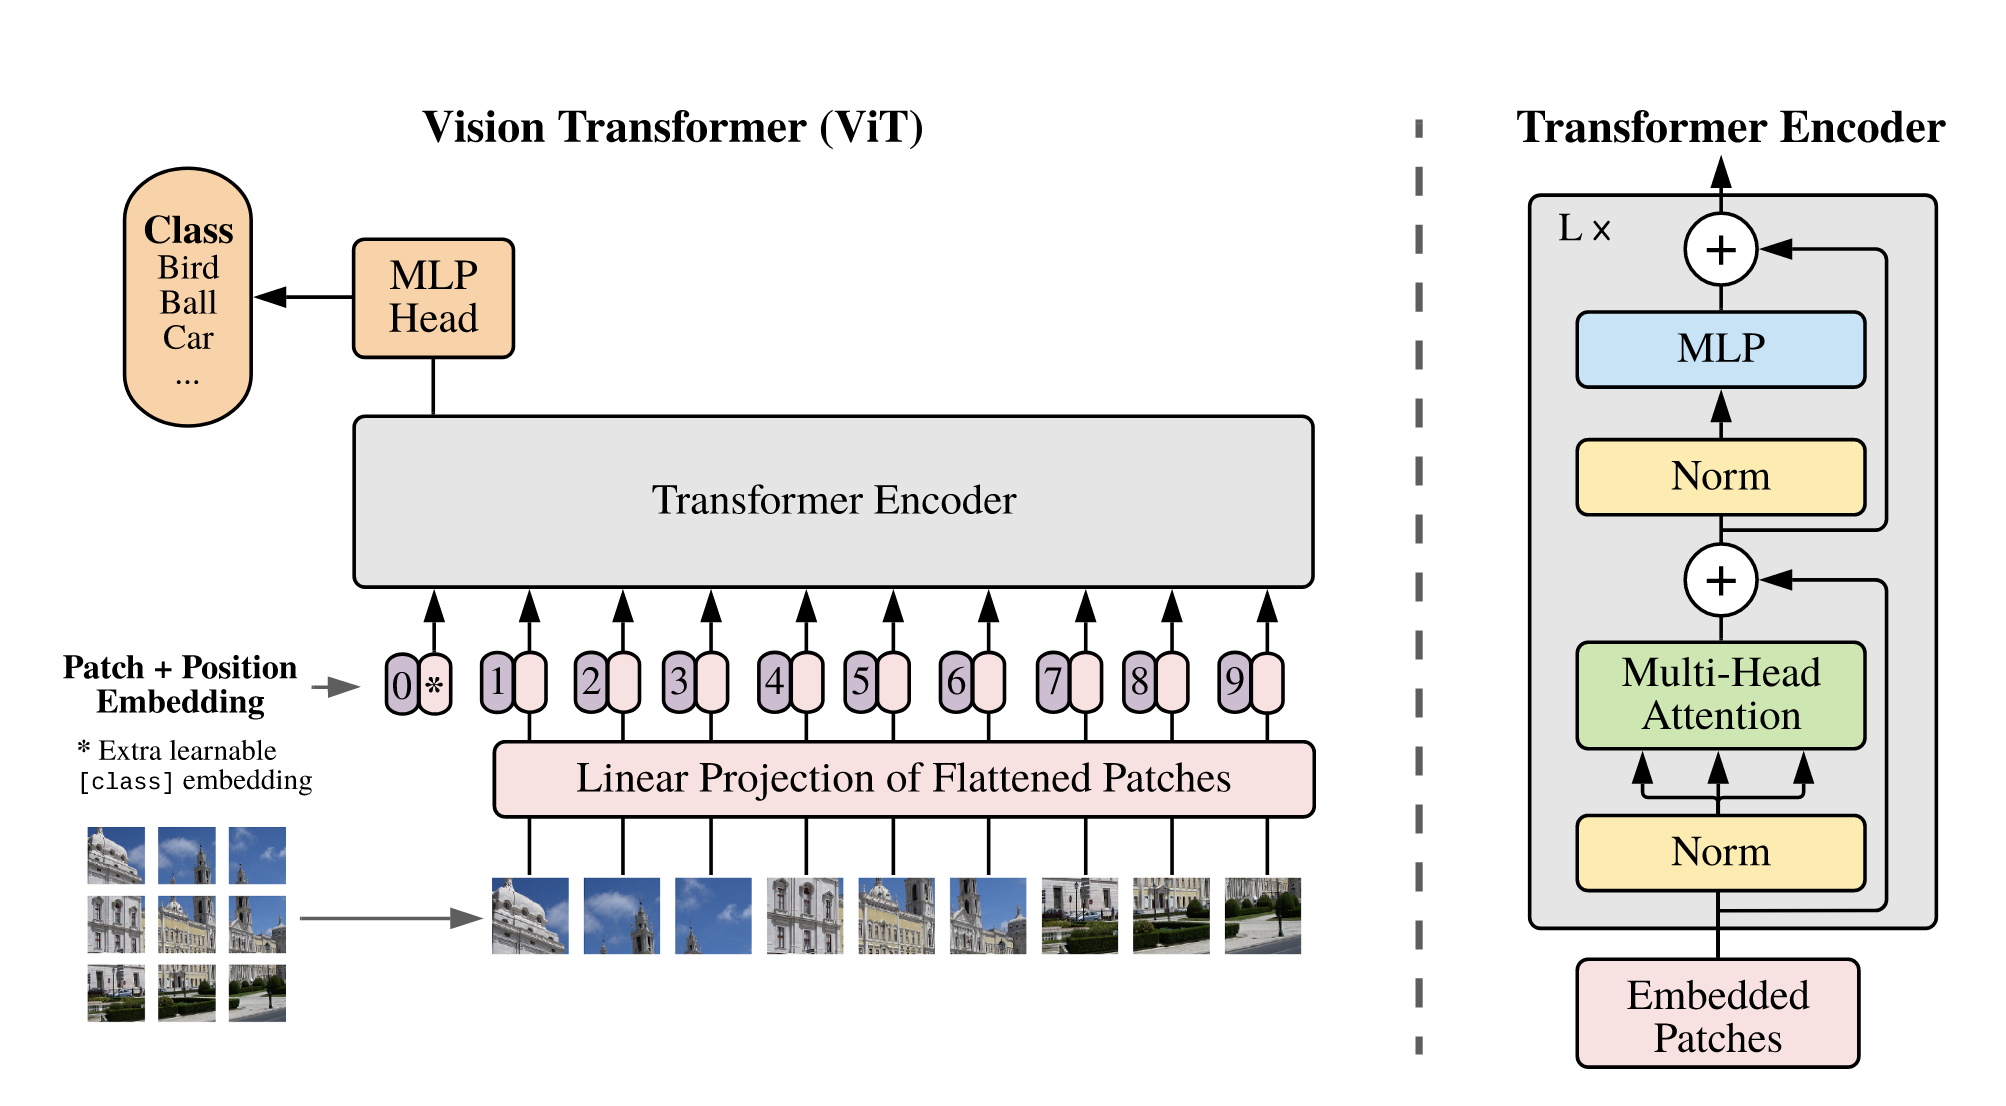
\includegraphics[width=\linewidth]{images/related/vit.png}
      \end{center}
      \caption{\textbf{The Vision Transformer (ViT):} the image is cropped without overlap and
            projected using a convolution whose stride equals the kernel size. The encoder is made
            of multiple transformer blocks. Finally, only the special learned token ``class token''
            is used at the end, and fed to a classifier (here denoted as the ``MLP Head''). Image
            from \cite{dosovitskiy2020vit}.}
      \label{fig:related_vit}
\end{figure}

This architecture is illustrated in \autoref{fig:related_vit}: we concatenare a special learned
token, called ``\textit{class token}'', to the patch tokens. Moreover, we also sum these tokens with
a learned position embedding to facilitate the learning of each token position. Then, successive
transformer blocks process all the tokens. Each block is made of LayerNorms \citep{ba2016layernorm},
a self-attention block, a \ac{MLP}, and residual connections. Thus, the self-attention block is:
%
\begin{equation}
      \begin{aligned}
            Q & =W_{q} \vx\,,                                                       \\
            K & =W_{k} \vx\,,                                                       \\
            V & =W_{v} \vx\,,                                                       \\
            A & =\operatorname{Softmax}\left(Q \cdot K^{T} / \sqrt{D / h}\right)\,, \\
            O & = W_{o} A V+b_{o}\,,
      \end{aligned}
      \label{sec:related_sa}
\end{equation}
%
\noindent $\vx$ are the $N$ patch tokens and the class token, of shape $(N, D)$, $D$ being the
embedding dimension. The patch tokens are linearly transformed three times in parallel into a
\textbf{Q}uery, \textbf{K}ey, and \textbf{V}alue. An attention matrix of shape $(N, N)$ is computed
from the query and the key. Its $i^{\text{th}}$ row contains the similarity between the
$i^{\text{th}}$ with all other tokens. Finally, the multiplication between the attention matrix and
the value matrix averages all tokens according to their similarities. To extend the self-attention
to its multi-heads variation (\ac{MHSA}), we use several Query/Key/Value transformations, each
used in a self-attention on a fraction of the embedding dimension.

ViT \citep{dosovitskiy2020vit} is the seminal paper on vision transformer. However, its training was
difficult and needed a large --- and private --- dataset called JFT300M. Later works, including DeiT
\citep{touvron2021deit} proposed an efficient optimization procedure enabling the training of
transformers on smaller datasets such as ImageNet \citep{russakovsky2015imagenet_ilsvrc}. Finally,
multiple works improved also the architecture itself, including CaiT \citep{touvron2021cait}, ConViT
\citep{dascoli2021convit}, and Swin \citep{liu2021swin}.

\section{Continual Learning}
\label{sec:related_continual}

Usually, when training a \ac{CNN}, we assume the dataset is immutable and \textit{i.i.d.}: no new
images nor new classes will be learned. The knowledge acquired on one dataset \textit{A} can be
\textit{transferred} to another dataset \textit{B} with different classes using \textbf{transfer learning}
\citep{razavian2014transferlearning}. Then, the new model may be efficient on
the classes of dataset \textit{B} but cannot predict anymore the classes of dataset \textit{A}.

\textbf{Continual Learning} aims to learn a continually changing dataset without forgetting the
previous knowledge. The distribution of the dataset continually changes: \eg at each time-step $t
\in \{1, ..., T \}$, new
classes or new samples from potentially new domains are added to the training dataset
\citep{lomonaco2017core50}. We usually assume the test dataset evolves similarly. Multiple
distribution drifts exist in Continual Learning
\citep{morenotorresa2012datasetshift,lesort2021driftanalysis}, and they have been called under
various names in the literature. Given an input sample $x$ and its ground-truth $y$ (a label in
image classification, or a segmentation map in semantic segmentation), the major drifts are:

\begin{itemize}
      \item \textbf{Covariate drift}: when $p(x)$ changes, it happens with the introduction of new
            domains \citep{volpi2021continualdomainadapt}
      \item \textbf{Prior drift}: when $p(y)$ changes; \ac{CIL} happens with this kind of drift.
      \item \textbf{Conceptual drift}: when $p(y | x)$ changes. Seldom covered in the literature, it
            can be found in \acf{CSS}.
\end{itemize}

Learning an ever-growing dataset is possible by training from scratch a new model on the union of
past and new data. However, for multiple reasons like privacy concerns of medical data or limited
storage capacity in embedded device \citep{vasquez2017incrementalneuralforest}, there is a
restriction on the amount of previous data that can be kept. In the extreme case, where a model only
has access to new data but not old data, a model trained from scratch cannot predict previous
iterations' distribution. Worse, even if the old model is kept and finetuned on the new data, it
will suffer from a significant drop of the performance on old data that we call \textbf{Catastrophic
      Forgetting} \citep{robins1995catastrophicforgetting}.

\begin{figure}[tb]
      \begin{center}
            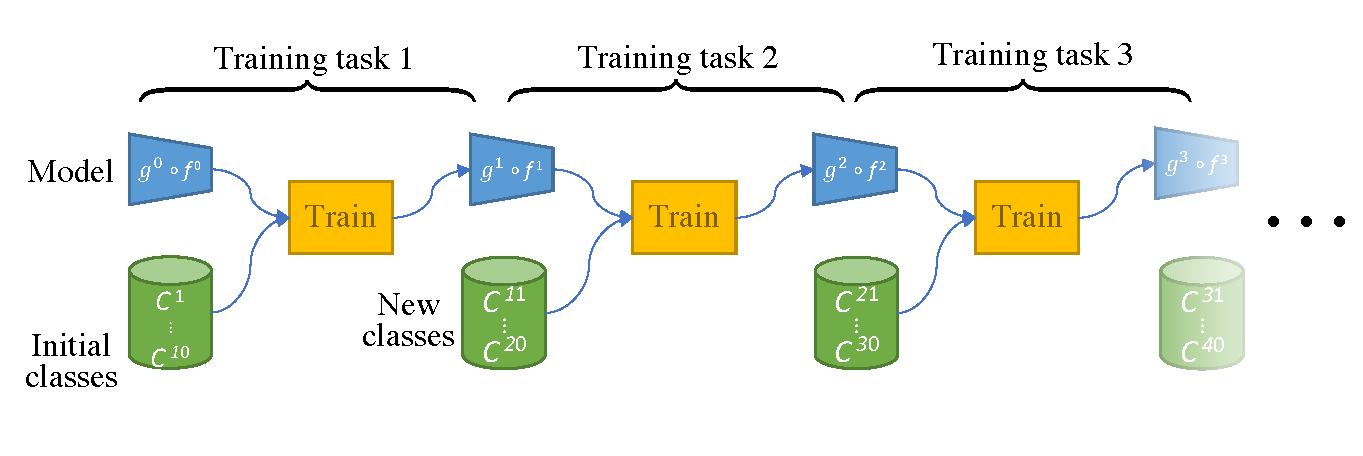
\includegraphics[width=1.0\linewidth]{images/related/protocol}
      \end{center}
      \caption{\textbf{Training protocol for incremental learning}. At each training task we learn a
            new set of classes, and the model must retain knowledge about \textit{all} classes. The
            model is allowed a \textit{limited} memory of samples of old classes.}
      \label{fig:related_protocol}
\end{figure}

\paragraph{Class-Incremental Example} More concretely, a common benchmark in \acf{CIL} is learning
the image classification CIFAR100 dataset \citep{krizhevskycifar100} in multiple steps, each made of
several new classes. \eg a model could learn at first to classify among 10 classes, then add 10 more
classes, \etc. Until it has learned all 100 classes. After each step, the model has to classify
among all classes it has learned. The \autoref{fig:related_protocol} illustrates such continual
protocol, and \autoref{fig:related_forgetting} depicts the performance of continual models in this
situation: the \textcolor{orange}{orange} line displays the accuracy of a model which is re-trained
from scratch at each step on all previous training data. This model, usually called Joint, is
considered as a reasonable upper bound. On the other hand, the \textcolor{blue}{blue} line is a
model finetuned solely on new classes without access to previous classes. The model's accuracy is
considerably lower than its Joint counterpart, because it forgets old classes by over-predicting new
classes. While we have mainly tackle \acf{CIL} benchmarks, we describe other continual benchmarks in
detail in the appendix (\autoref{sec:related_variation}).

\paragraph{Single-Head \vs Multi-Heads} are the two main evaluation settings in Continual Learning
\citep{chaudhry2018riemannien_walk}. In the former setting, a model has to classify samples among
all seen classes, that could have been learned from any of the seen steps. The latter setting knows
at test-time the step/task identifier of the samples. Thus, it only has to classify among the limited
number of classes brought by a step. This setting is closely related to multi-tasks learning. During
this thesis, we focus on the Single-Head setting because it is more realistic as it is not always
possible to know from which step a sample comes from in a real-life setting, and more challenging
\citep{lesort2019regulshortcomings}.

\begin{figure}[tb]
      \begin{center}
            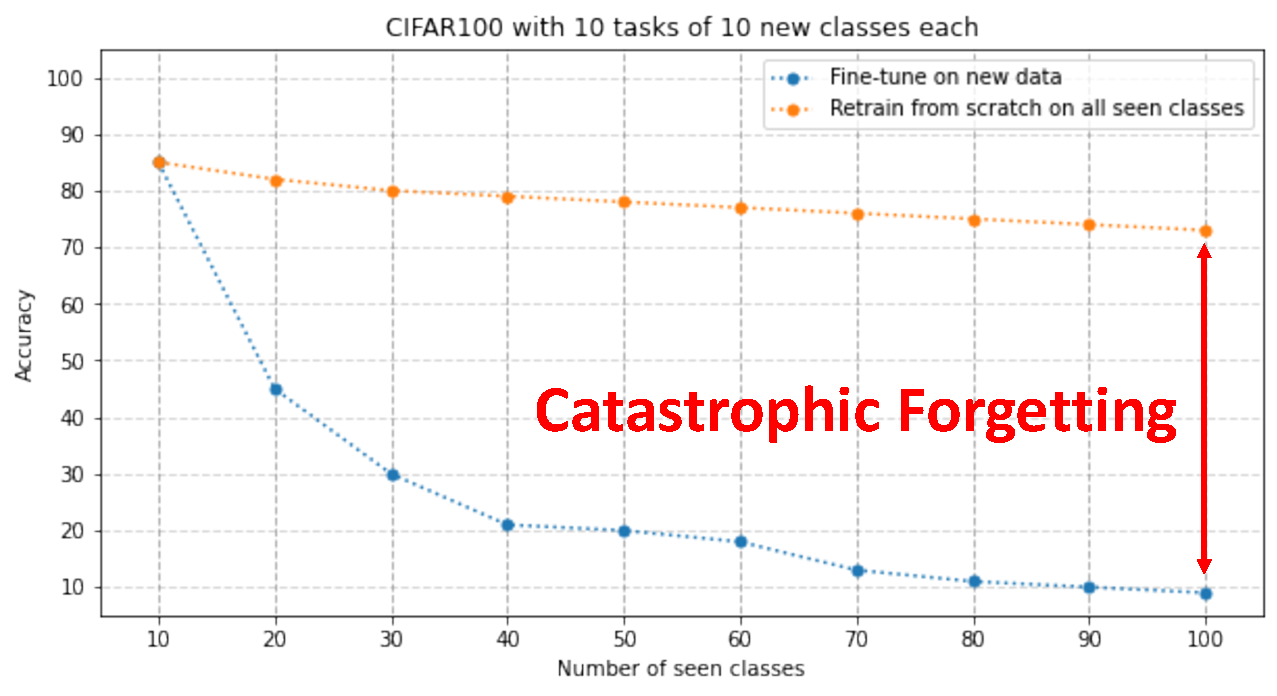
\includegraphics[width=0.8\linewidth]{images/related/catastrophic_forgetting.pdf}
      \end{center}
      \caption{\textbf{Training protocol for incremental learning}. At each training task we learn a
            new set of classes, and the model must retain knowledge about \textit{all} classes
            despite having no more access to old classes.}
      \label{fig:related_forgetting}
\end{figure}


%\subsection{Metrics for Continual Learning}
\label{sec:related_metrics}

\paragraph{Metrics} Multiple metrics exist in Continual Learning: the most common are the \textbf{final accuracy} and
\textbf{average incremental accuracy}. The former measures the performance of the model on all tasks
at the last step, the latter measures the average of performance on all seen tasks after each new
task learned \citep{rebuffi2017icarl}. Practically, given $A_{i,t}$ the accuracy of the $i^{th}$
task after
learning the $t^{th}$ task, the final accuracy is (assuming balanced tasks):
%
\begin{equation}
      \text{Acc}_F = \frac{1}{T} \sum_{i=1}^T A_{i,T}\,,
      \label{eq:related_final_acc}
\end{equation}
%
and the average incremental accuracy:
%
\begin{equation}
      \text{Acc}_a = \frac{1}{T} \sum_{t=1}^T \frac{1}{t}  \sum_{i=1}^t A_{i,t}\,.
      \label{eq:related_avg_acc}
\end{equation}
%
Average incremental accuracy is somewhat more important than simply the final accuracy: a continual
model should be good after every step because in a true continual setting, there is not a ``final
task''.

Other metrics exist \citep{diaz2018continualmetrics}, including the \textbf{backward and
      forward transfer} \citep{lopezpaz2017gem} that measures the influence that learning a task has on
the performance of respectively past and future tasks. Another notable metric is the
\textbf{forgetting} \citep{chaudhry2018riemannien_walk} which records how much a model has lost
performance-wise on a task compared to the first time it has learned it. The interest of this metric
is to be agnostic of the absolute performance of the model used.

Finally, metrics such as \textbf{speed} (\ie the number of images processed per second) or used
\textbf{capacity} (\ie number of learned parameters) are important:
\cite{ramasesh2022scalecontinual} recently showed that the larger a model was the lower was the
forgetting.

\section{Methods to reduce forgetting}
\label{sec:related_methods}

Multiple approaches exist to reduce forgetting in Continual Learning. The major ones are
rehearsal of old data (\autoref{sec:related_rehearsal}), regularizations constraining the model's
behavior (\autoref{sec:related_regul}), and structural adaptations (\autoref{sec:related_structural}).

\subsection{Rehearsal Learning}
\label{sec:related_rehearsal}

The most efficient method to reduce forgetting is \textbf{rehearsal learning} where old samples will
be seen alongside the new samples. The amount of old samples stored is extremely limited, otherwise,
it would defeat the purpose of continual learning. \autoref{fig:related_protocol_rehearsal} illustrates how
rehearsal learning happens in Continual Learning. During the first step, a model is trained on all
available samples. Then, it stores a limited amount of those in a \textit{memory}. During the second
step, the model has access to new samples but also all samples stored in the memory. In
Class-Incremental, an equal amount of samples per class is stored in memory. There are
two major approaches to determine this amount: \cite{rebuffi2017icarl} propose to fully use a
memory of size $\mcM$ among all $\mcC$, while \cite{hou2019ucir} instead kept fixed the number of
samples stored per class to $\nicefrac{\mcM}{|\mcC^{1:T}|}$.

\paragraph{Herding} is the action of choosing which samples per class to store in the rehearsal
memory. The most naive herding method is to randomly sample images. Despite its simplicity, it is
quite competitive with more complex method \citep{castro2018end_to_end_inc_learn}, echoing similar
results in \ac{AL} \citep{gal2017activelearning}. Other herding methods include fetching samples
close to the class mean in the feature space \citep{castro2018end_to_end_inc_learn} or close to an
incremental barycenter \citep{rebuffi2017icarl}.

\paragraph{Sampling} is an important but yet fewly investigated topic in Continual Learning. Most
models mix all memory samples with new samples without any under- or over-sampling.
\cite{castro2018end_to_end_inc_learn} propose to finetune for a few epochs, after training on a new
step, on a balanced set of old and new classes samples. \cite{chaudhry2019tinyepisodicmemories}
oversample tiny memory with as low as one sample per class, and show, in the context of Online
Learning where models learn in only one epoch, that continual models still do not overfit. In the
same context, \cite{aljundi2019maximallyinterfered} propose to over-sample the memory examples with
the highest losses. In an imbalanced situation for Continual Learning, over- and under-sampling can be
applied depending on the number of samples per class \citep{kim2020imbalancedcontinual}.

\paragraph{Efficient Storing} is important for rehearsal learning: a bigger rehearsal memory leads
invariably to less forgetting \citep{hou2019ucir}. Thus, multiple works consider how to store more
rehearsal sampes given the same memory size: \cite{hayes2020remind} compress intermediate features
of memory samples with a lossless compression algorithm.
\cite{iscen2020incrementalfeatureadaptation} also store features but modify them through the
training to handle the inherent internal covariate drift.

\paragraph{Pseudo-rehearsal} does not need to store samples but instead generates pseudo-samples for
rehearsal \citep{lesort2019generative}. The generation can be done with auto-encoders from
intermediate features \citep{kemker2018fearnet,ayub2021eec} or use \ac{GAN}
\citep{shin2017deep_generative_replay}. Unfortunately, those methods have several drawbacks: they
struggle to scale to large images, the generator size may be superior to a classic rehearsal memory
size which would defeat the goal of using less storage, and finally, the generator may itself suffer
from catastrophic forgetting \citep{zhai2019lifelonggan}. \cite{liu2020mnemonics} propose instead a
method halfway between rehearsal and pseudo-rehearsal: the authors sample randomly real images, and
then during continual training, slightly modify them via bi-level optimization
\citep{wang2018datasetdistillation} to minimize forgetting.


\begin{figure}[tb]
      \begin{center}
            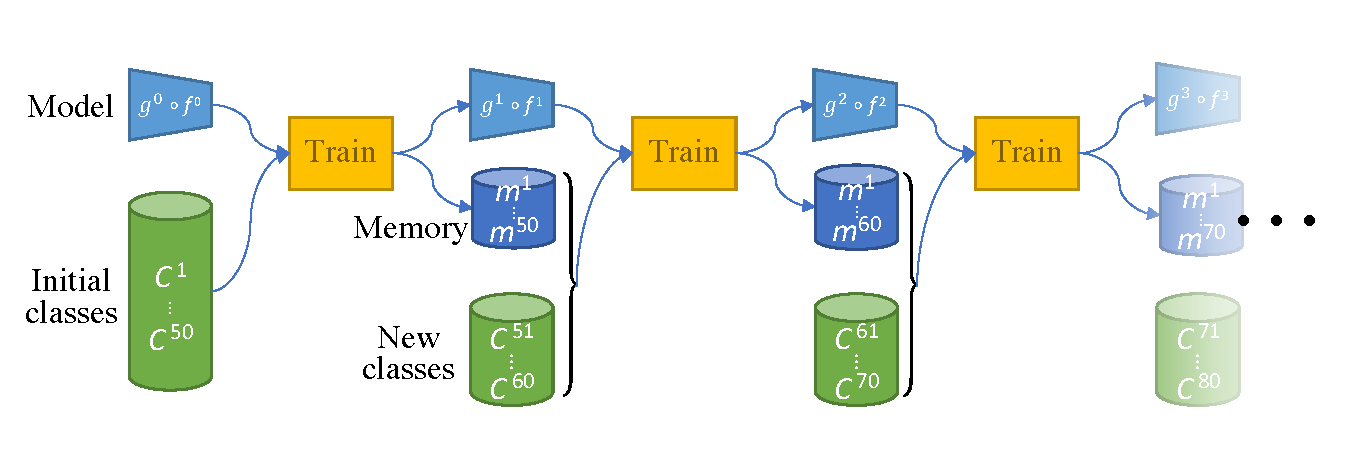
\includegraphics[width=1.0\linewidth]{images/related/rehearsal}
      \end{center}
      \caption{\textbf{Training with a rehearsal memory}. After each task a fraction of the
            data is stored in a memory to be used in the next task. Rehearsal learning is the most
            efficient method to reduce forgetting, but unfortunately the memory capacity is often
            extremely limited.}
      \label{fig:related_protocol_rehearsal}
\end{figure}

\subsection{Regularization-based Approaches}
\label{sec:related_regul}


\begin{figure}[tb]
      \begin{center}
            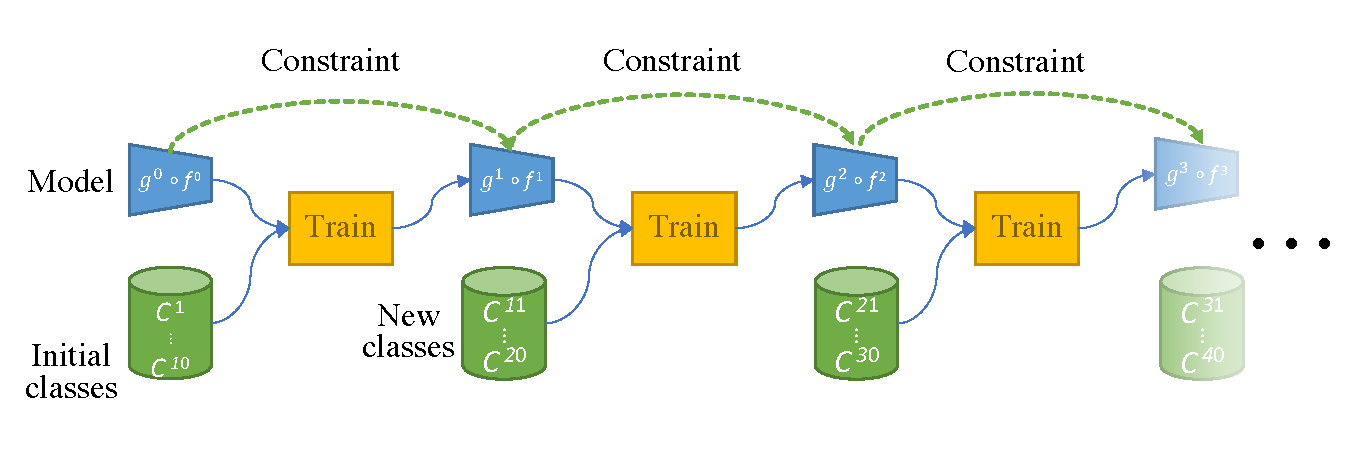
\includegraphics[width=1.0\linewidth]{images/related/constraints}
      \end{center}
      \caption{\textbf{Constraining the new model based on the old model}. During each task, after
            the first one, the new model is constrained to be similar to the old model in order to reduce
            forgetting.}
      \label{fig:related_protocol_constraints}
\end{figure}

A common and efficient way to reduce forgetting, is to minimize the difference in behavior between
the old and new models as illustrated in \autoref{fig:related_protocol_constraints}. These constraints can be
expressed through various forms and are described below.

\subsubsection{Weight-based constraints}
\label{sec:related_regul_weight}


The most straightforward way to avoid completely forgetting, is that the old and new models stay
identical. While the model would be \textit{rigid} (no forgetting), it is also not \textit{plastic}
(changing a lot) at all, and thus cannot learn any new tasks. Thus, a line of research proposed to
constrain only a portion of the neurons:
%
\begin{equation}
      \mcL(\theta^t, \theta^{t-1}) = \mcL_t(\theta^t) + \lambda \sum_i \Omega_i^{t-1} (\theta^t_i - \theta_i^{t-1})^2\,,
      \label{eq:related_weight_constraint}
\end{equation}
%
where $\mcL_t(\theta)$ is the loss at the current task $t$ (\eg the cross-entropy), $\theta_i^t$
and $\theta_i^{t-1}$ respectively the $i^\text{th}$ neuron of the current and previous model, and
$\Omega_i^{t-1}$ a neuron-wise importance factor. The intuition is that important neuron for the
previous task $t-1$ should not change, while the others can be adapted to fit the new task $t$.

\cite{kirkpatrick2017ewc}, followed by \cite{zenke2017synaptic_intelligence} and
\cite{chaudhry2018riemannien_walk} propose to use the diagonal Fisher information matrix as
importance factors. The motivation behind was that the posterior $p(\theta^{t-1} | \mcD^{t-1})$ must
contain the information about which parameters are important to the previous dataset $\mcD^{t-1}$.
This posterior can be approximated by a Gaussian distribution whose diagonal precision is given by
diagonal Fisher information matrix. A higher value means a more important neuron for the previous
task, and thus the constraint should be increased proportionally. Thus, a lower value, for a less
important neuron, means that it can change drastically, which would facilitate learning new data.
This strikes a balance between rigidity (not changing and thus not forgetting), and plasticity
(changing, and thus learning new concepts). Note that \cite{aljundi2018MemoryAwareSynapses} instead
use the sensitivity of the model when small perturbations are added to the neurons to measure their
importance.

However, it is worth remarking that weight-based constraints are usually limited to the multi-heads
setting where a task identifier is available at test time. \cite{lesort2019regulshortcomings} show
that in the single-head setting, they struggle to reduce forgetting and are significantly
outperformed by the simple (but somewhat memory costly) rehearsal learning.

\subsubsection{Gradient-Based methods}
\label{sec:related_regul_gradient}

\begin{figure}[tb]
      \begin{center}
            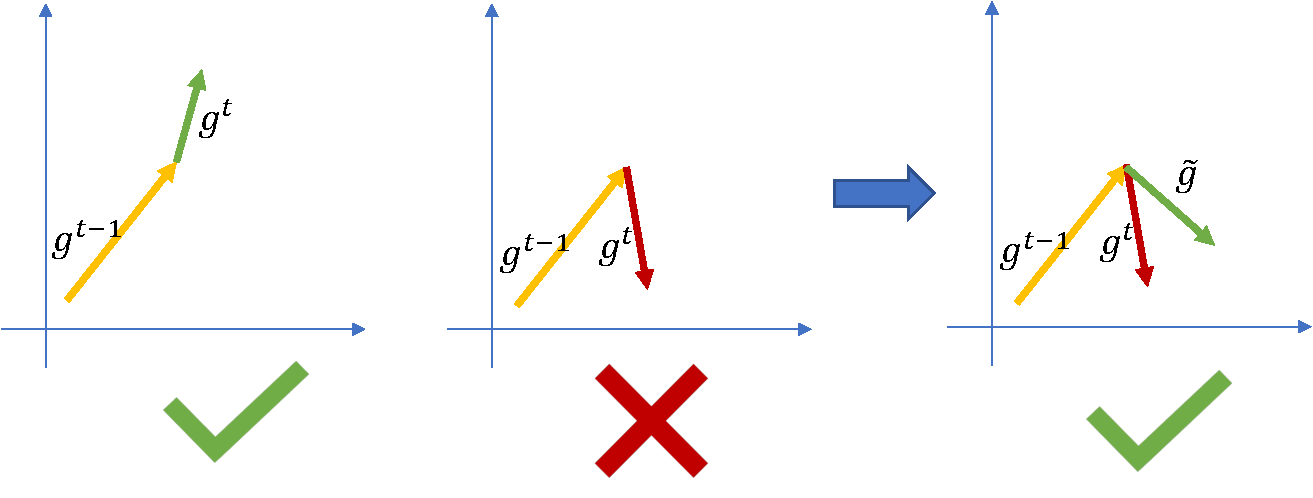
\includegraphics[width=1.0\linewidth]{images/related/gem.pdf}
      \end{center}
      \caption{\textbf{GEM's gradient constraint} forcing updates to be in the same direction as the
            gradient \wrt old samples.}
      \label{fig:related_gem}
\end{figure}

\cite{lopezpaz2017gem} propose the GEM model that combines a constraint on the gradients and
rehearsal learning. The algorithm requires that the loss on a given stored sample must not increase
despite the model learning new classes. The authors, given a locality assumption, rewrite this
formulation as enforcing that the gradient of a new sample ($g$) to be in the same \textit{direction} as
the gradient of a stored old sample ($g_i$):
%
\begin{equation}
      \langle g,\, g_i\rangle \ge 0,\, \text{for all}\, i \in \mcM\,,
\end{equation}
%
\noindent with $\mcM$ the rehearsal memory. If the constraint is violated, the new gradient $g$ is
projected to the closest in L2 norm gradient that satisfies the angle constraint by minimizing a
quadratic program. The constraint is illustrated in \autoref{fig:related_gem}. The drawback of this
method is the computational cost that can grow prohibitively when the memory is too large.
\cite{chaudhry2019AGEM} propose Averaged-GEM to speed up GEM: the authors do not constraint the
gradient of individual memory samples but only the average of all memory samples.
\cite{aljundi2019gradientselection} also improved GEM's speed by selecting only a subset of the
memory samples that maximize the feasible region.

Differently, but still constraining the gradients: \cite{farajtabar2020ogd}'s OGD forces the gradients of
task $t$ to be orthogonal to gradients of task $t-1$. They use the Gram-Schmidt procedure to
orthogonalize the new gradients, allowing updates for the new task that minimally interfere with the
performance of old tasks. \cite{saha2021gpm}'s GPM does likewise but uses instead a k-rank
approximation of the SVD of the representation matrix.


\subsubsection{Output-based constraints regularizations}
\label{sec:related_regul_output}

Finally, the majority of Continual models that are benchmarked on large datasets (\eg ImageNet
\citep{deng2009imagenet}) use a combination of rehearsal
learning (\autoref{sec:related_rehearsal}) and constraints on the model's outputs.

LwF \citep{li2018lwf} and iCaRL \citep{rebuffi2017icarl} apply the \ac{KD}
\citep{hinton2015knowledge_distillation} on the model's probabilities. It usually consists in
minimizing the \ac{KL} between the probabilities of the old and new models:
%
\begin{equation}
      \mcL_\text{KD} = \operatorname{KL}(\operatorname{softmax}(\frac{\tilde{y}^{t-1}}{\tau}) \Vert \operatorname{softmax}(\frac{\tilde{y}^t}{\tau})\,,
\end{equation}
%
where $\tilde{y}^{t-1} = g^{t-1} (f^{t-1}(\vx))$ and $\tilde{y}^{t} = = g^{t} (f^{t}(\vx))$ are respectively the logits of the old and new model,
and $\tau$ a \textit{temperature} to soften the probabilities in order to give more importance to
the model confidence in other classes than the top one. These probabilities, nicknamed \textit{dark
knowledge} by \cite{hinton2015knowledge_distillation}, contain additional information about the
model which are useful to distil. Note that in the context of Class-Incremental, the new model
predicts more classes than the old model, therefore, the \ac{KL} is only applied on the logits
common to both the old and the new models. The \ac{KD} is sometimes also defined as the binary
cross-entropy between the sigmoid-activated logits.

Constraining the probabilities is now so ubiquitous that most models include it in their base
losses. On the other hand, a few models considered constraining intermediate outputs. MK2D
\citep{peng2019m2kd} uses the \ac{KD} from both the final classifier and an auxiliary classifier
similarly to the Inception network \citep{szegedy2015inception}. \cite{hou2019ucir} maximize the
cosine similarity between the embeddings produced by the \ac{GAP}.
\cite{dhar2019learning_without_memorizing_gradcam} minimizes the L1 distance between the attention
maps produced by GradCam \citep{selvaraju2017gradcam}.

\subsection{Structural Strategies}
\label{sec:related_structural}

\begin{figure}[tb]
      \begin{center}
            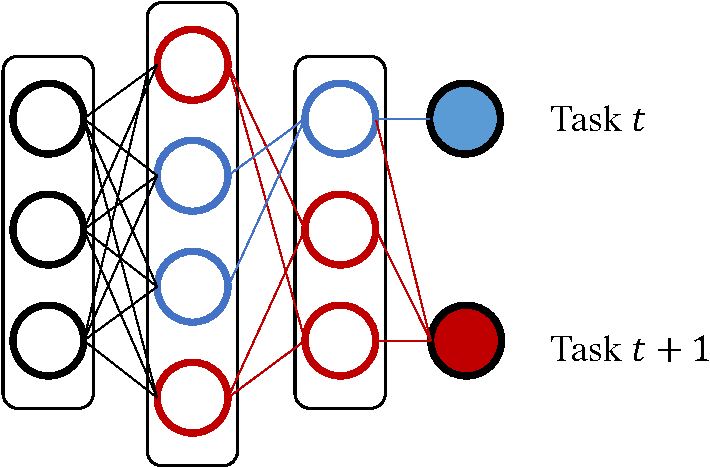
\includegraphics[width=0.6\linewidth]{images/related/subnetworks.pdf}
      \end{center}
      \caption{\textbf{Task-specific subnetworks} that can be uncovered with a sparsity loss or
            learned masking.}
      \label{fig:related_subnetwork}
\end{figure}

Multiple works have also propose to adopt dynamic strategies where the configuration of the neural
network evolves after each task. Critically, not only the number of neurons change in the classifier $g^t$
(to incoporate new classes to predict), but the feature extractor $f^t$'s neurons count or organization
will also differ from its previous iteration $f^{t-1}$.


\paragraph{Subnetworks} The Lottery Ticket Hypothesis \citep{frankle2019lottery_ticket} states that
subnetworks, made of a fraction of the neurons and connections of a larger network, can reach
excellent performance. Several Continual Learning models exploit that property by using a
subnetwork per task. Those subnetworks can be uncovered via genetic algorithms
\citep{fernando2017path_net}, via induced L1 sparsity \citep{golkar2019neural_pruning}, or even
learned masked \cite{serra2018hat,hung2019cpg}. Usually, these methods require a task identifier at
test-time in order to select the right subnetwork (see \textit{multi-heads} in
\autoref{sec:related_continual}). Later, \cite{wortsman2020supermasks} propose to infer the task
identifier by selecting the subnetwork with the lowest entropy. This subnetwork-based approach is
illustrated in \autoref{fig:related_subnetwork}.

\paragraph{Expandable Networks} A neural network can also be expanded through its continual
training to accommodate the growing amount of tasks to solve. First, \cite{rusu2016progressive}
propose to have one network per task, where the $i^{\text{th}}$ network would depend both on the
input and all previous networks' intermediate features. Unfortunately, the memory consumption is
quickly prohibitive with many tasks. Following works propose to only add blocks of parameters,
and only when deemed necessary



\paragraph{Task Conditioning} Rather than adding many new parameters, it is also possible to only
add a few parameters that will adapt the existing network behavior for a task.
\cite{rebuffi2017visualadapters} propose to add a different residual per task: given a task
identifier, the associated residual is used, and the features are modulated to best fit the given
task. Instead of adapting the features, \cite{wen2020batchensemble} and \cite{sun2019metatransfer}
propose to share most of the weights across tasks, but have task-specific weights that directly
modify the shared weights.

\paragraph{Mixture-of-Experts} Mixture of experts \citep{masoudnia2014mixture} have also been
proposed, where multiple experts combine their decision. \cite{aljundi2017experts} learn a gating
system to use the right task-specific expert.
%\cite{yan2021der} and \cite{li2021preserve} proposed
%to have a \ac{ConvNet} per task and to concatenate their output embeddings to be fed to a single
%classifier. To avoid parameters explosion, they aggressively prune each \ac{ConvNet}.

\paragraph{Classifier Correction} Forgetting happens in both the feature extractor and the
classifier. Previously described rehearsal and regularization methods try to reduce it in both
places. On the other hand, multiple works focus solely on the classifier. They remark that in
\acf{CIL}, the classifier is miscalibrated \citep{guo2017miscalibration} where the model
over-predicts new classes to the detriment of old classes. \cite{belouadah2019il2m} compensate the
bias towards new classes by rectifying predictions of past classes using their recorded accuracies
and confidences. \cite{wu2019bias_correction} learn a linear model on validation data to recalibrate
the logits of the new classes. \cite{zhao2020weightalignement} normalizes the norm of the classifier
weights associated with new classes so that their average norm becomes the same as that for old
classes. \cite{hou2019ucir}, aims for a similar result by replacing the dot product in the
classifier by the cosine similarity, resulting in unit norm classifier weights.

\section{Positioning}

Continual Learning encompasses very different benchmarks and methods. In this thesis, we tackle
multiple types of continual drift using different approaches summarized below:

\paragraph{Feature-based Regularizations} First in \autoref{chapter:regularization}, we consider
\acf{CIL} scenarios with a prior drift where new classes are continually added. This is a
challenging benchmark, even more when tackling a large amount of classes with datasets like CIFAR100
(100 classes) and ImageNet (1000 classes). The previous State-of-the-Art models all use a
combination of rehearsal (\autoref{sec:related_rehearsal}) and regularizations of the predicted
probabilities (\autoref{sec:related_regul_output}). In this chapter, we claim that this type of
constraints struggle to efficiently balance the rigidity needed to not forget with the plasticity
required to learn new classes. Therefore, we propose to regularize, not the final outputs, but
rather the intermediate feature space. In the first section (\autoref{sec:podnet}), we describe how
we regularize statistics on the features at multiple levels of the \ac{ConvNet} with our method
called POD. The choice of which statistics to employ has an important impact on forgetting, which I
ablate extensively. While this first section aims to constrain the feature space to reduce
forgetting, the second section (\autoref{sec:ghost}) tries to avoid forgetting before it even
happen: Inspired by \ac{ZSL}, we estimate the feature representation of future classes using weak
information about them (\eg attributes). Exclusion zones in the feature space are created for those
yet unseen classes, so that when finally learned, the confusion between old and new classes is
minimal.

\paragraph{Continual Semantic Segmentation} Second, in \autoref{chapter:segmentation}, we tackle
\acf{CSS}. In this benchmark, images have a label per pixel, and only the current classes are
labelized. Thus, both the prior and concept drifts happen where new classes are added but also the
signification of a pixel can change through time. Three different, but complementary, methods are
used for this type of data: first we use an uncertainty-based pseudo-labeling to handle what we
called a background shift. Then, we extend the feature regularization
(\autoref{sec:related_regul_output}) introduced in the previous chapter, POD, to constrain
differently local and global areas of the spatial feature maps. Finally, we consider rehearsal
learning (\autoref{sec:related_rehearsal}) propose a new rehearsal, designed for segmentation, by
exploiting a copy-paste of masks resulting in State-of-the-Art performance while being very memory
efficient.

\paragraph{Dynamic Transformers} In this third and last chapter (\autoref{chapter:dynamic}), we only
aim to solve the prior drift but using a method radically different from previous chapters: dynamic
networks (\autoref{sec:related_structural}). Previous dynamic networks usually expand their
capacity by a large margin during the continual training to handle the growing amount of tasks to
learn. To avoid a parameter count explosion, the models are usually pruned aggressively. The main
drawback of these methods is that the pruning can still result in models too large and often need
careful finetuning of hyperparameters. We propose in this chapter, a novel dynamic expansion with
almost no memory overhead contrary to concurrent works. Based on the transformer architecture, a
special learned vector is used per task to specialize the features to each task. Consequently,
forgetting is greatly reduced while our memory and time overheads stay manageable.

\cleardoublepage
\let\leftmark=\oldleftmark

\acresetall
\chapter{Regularization-based Models}
\label{chapter:regularization}

%\minitoc
\chapterwithfigures{\nameref*{chapter:regularization}}
%\chapterwithtables{\nameref*{chapter:introduction}}

\ifthenelse{\boolean{skipRegul}}{\endinput}{}

\section{Introduction}

\section{PODNet: reducing forgetting}

\subsection{Model}

\subsection{Experiment results}


\section{Ghost: avoid pre-emptively forgetting}

\subsection{Prescient Continual Learning}

\subsection{Model}

\subsection{Experiment results}


\section{Conclusion}


\cleardoublepage
\let\leftmark=\oldleftmark

\acresetall
\chapter{Continual Segmentation}
\label{chapter:segmentation}

\begin{chapabstract}
    In \acf{CIL}, new classes are learned with each new task. However, most of the literature in
    that domain focus on image classification, where a single label is possible per sample. In
    \textbf{\acf{CSS}}, the setting is the same (continual addition of new classes), but the implications are wildly different. In Semantic
    Segmentation, an image has one label per pixel. Therefore, an image could contain pixels from
    old, current, and future classes.
    \\
    In this chapter, we tackle the recent field of \acf{CSS}: We first highlight the main
    challenges of this domain: an important \textbf{catastrophic forgetting} linked to the higher complexity
    of segmentation images, and a \textbf{background shift} where images are partially labeled with
    only the current classes' ground-truth being present. Then, we propose multiple complementary
    methods across two papers to solve those challenges: We design an uncertainty-based
    hard pseudo-labeling loss, a multi-scale distillation loss inspired by our previous POD, and
    an efficient object rehearsal method.

    The work in this section has led to two papers:

    \begin{itemize}
        \item \fullcite{douillard2020plop}
        \item \fullcite{douillard2021objectrehearsal}
    \end{itemize}

\end{chapabstract}
\newpage

\minitoc
\chapterwithfigures{\nameref*{chapter:segmentation}}
\chapterwithtables{\nameref*{chapter:segmentation}}

\ifthenelse{\boolean{skipSegm}}{\endinput}{}


\section{Introduction}
\label{sec:seg_intro}

Semantic segmentation aims to assign a label to each pixel of an image.
It allows the prediction of multiple objects in the same image, and moreover, their exact position
and shape. This task recently flourished \citep{tao2020HRNet,zhang2020resnest,chen2018ZPSA} with
larger datasets with thousands of fully annotated images
\citep{zhou2017adedataset,neuhold2017mapillary}, increased computational power, and larger attention
\citep{wang2020axialdeeplab}. Unfortunately, the recent research in this area is often impracticable
for real-life applications: they mostly \textbf{need fully annotated data and require to be retrained from
    scratch if a new class is added to the dataset.} Ideally, one would wish to regularly expand a
dataset, only adding and labeling new classes and updating the model in accordance. This setup,
referred here as \textbf{\acf{CSS}}, has emerged very recently for specialized
applications
\citep{ozdemir2018learnthenewkeeptheold,ozdemir2019segmentationanotomical,tasar19incrementsegmentationremotesensing}
before being proposed for general segmentation datasets
\citep{michieli2019ilt,cermelli2020modelingthebackground}.


In particular, in this chapter, we argue that two problems arise when performing \ac{CSS} with
\acs{DCNN}. The first one, inherited from continual learning, is \textbf{catastrophic
    forgetting}~\citep{robins1995catastrophicforgetting}, already well detailed in the previous chapters
including \autoref{chapter:related}. One of the most efficient methods to avoid forgetting is rehearsal
learning (\autoref{sec:related_rehearsal}) where we store a few images from previous tasks.
Unfortunately, this solution has difficulty in the context of segmentation where multiple classes
can be in the same image, and where the storage cost is high and images are partially labeled. The
second challenge, specific to \ac{CSS}, is the semantic shift of the background class. In a
traditional semantic segmentation setup, all object categories are predefined, and the "background"
class contains pixels that do not belong to any of these classes. However, in \ac{CSS}, the
background contains pixels that do not belong to any of the \textit{current} classes. Thus, for a
specific learning step, the background can contain both future classes, not yet seen by the model,
as well as old classes. Thus, if nothing is done to distinguish pixels belonging to the real
background class from old class pixels, this \textbf{background shift} phenomenon risks exacerbating
the catastrophic forgetting even further \citep{cermelli2020modelingthebackground}. This issue also
has an impact on the selection of the old data we want to store. Because some currently learned
classes are annotated as background in the old data, this may degrade the performance of these
classes if one naively treat them as background to fine-tune the current model.

We tackle the first challenge of catastrophic forgetting by designing a constraint enforcing a
similar behavior between the old and current models. Specifically, we leverage intermediary
representations of the convolutional networks to ensure that similar patterns are extracted through
time. \textbf{This feature-based constraints, called Local POD, fully exploits the global and local
    scale necessary to semantic segmentation through a multi-scale design}. The second challenge,
background shift, is greatly alleviated \textbf{a confidence-based pseudo-labeling strategy to
    retrieve old class pixels within the background}. For instance, if a current ground truth mask only
distinguishes pixels from class \texttt{sofa} and background, our approach allows assigning old
classes to background pixels, \eg classes \texttt{person}, \texttt{dog} or \texttt{background} (the
semantic class). We name PLOP the model exploiting those two contributions. We then propose
\textbf{an extension called PLOPLong that aims to excel on long continual learning scenarios}. This
new model exploits cosine normalization to adapt the classifier and the Local POD resulting in
improving robustness to the discrepancy between old and new classes. Moreover, PLOPLong features a
modified batch normalization which reduces the sensitivity of the model to moving statistics seen
across tasks in continual learning. Finally, we are the first to investigate rehearsal learning in
the frame of \ac{CSS}. We propose a baseline approach that is based upon rehearsing complete images.
However, in practice, this seemingly classic rehearsal is not as trivial in our context as the
labeling is partial: hence, once again, we need to complete the rehearsed images after each step by
filling the background with the missing old classes. While significantly improving performances, we
show that such approach has two main drawbacks. First, it is memory intensive, as the whole images
shall be rehearsed at each \ac{CSS} step. Second, despite a large number of pixels in the images,
we argue that the images contain few, sparse useful information. Consequently, we design \textbf{a
    novel rehearsal method, that we named ``Object Rehearsal``, that consists in selecting only
    non-regular objects-centered patches as candidates for rehearsal}. Those objects, belonging to old
classes, are combined into the images of new classes \textit{via} careful image editing. We
empirically show that this new rehearsal method surpasses classic rehearsal with pseudo-labeling,
while being up to 146x times more memory efficient.

From a practical point of view, our proposed methods (PLOP, PLOPLong, and Object Rehearsal) showed
three important results. First, we achieve the state-of-the-art performance on several challenging
datasets. Secondly, we propose several novel scenarios to further quantify the performances of \ac{CSS}
methods when it comes to long term learning, class presentation order, and domain shift. Last but not
least, we show that our model contributions largely outperform every \ac{CSS} approach in these
scenarios.

To sum it up, our contributions are four-folds:
\begin{itemize}
    \item We propose a multi-scale spatial distillation loss to better retain knowledge through the
          continual learning steps, by preserving long- and short-range spatial statistics, avoiding
          catastrophic forgetting.
    \item We introduce a confidence-based pseudo-labeling strategy to identify old classes for the
          current background pixels and deal with background shift.
    \item We propose PLOPLong, a carefully designed refinement of our method for dealing with long
          \ac{CSS} scenarios. The extension comes from an adaptation of PLOP's classifier and Local POD
          distillation as well as batch re-normalization for better handling of both catastrophic
          forgetting and background shift, respectively.
    \item We design a novel memory-efficient Object rehearsal learning procedure that consists in
          storing and carefully pasting objects through selective erasing of foreground objects. It
          results in better performance for a fraction of the memory cost imposed by classic
          rehearsal.
\end{itemize}

Additionally, We show that our PLOP significantly outperforms state-of-the-art approaches in existing
scenarios and datasets for \ac{CSS}, as well as in several newly proposed challenging benchmarks on new
datasets. Furthermore, we show that PLOPLong leads to superior performances on longer \ac{CSS} scenarios.
Last but not least, we show that \ac{CSS} models' performance can be greatly improved where rehearsal
learning is an option. In such cases, the proposed Object rehearsal allows reaching high accuracies
with a small memory footprint.

\section{Related Work}
\label{sec:seg_related}

Continual Semantic Segmentation is a relatively young field that started getting traction following
\cite{michieli2019ilt} and \cite{cermelli2020modelingthebackground}. However, this field is at the
intersection of many popular topics. Therefore, we start this section with an overview of recent
advances in segmentation. We then follow with a more in-depth discussion of existing approaches to
\ac{CSS}. For a thorough discussion of Continual Learning, please refer to
\autoref{chapter:related}.

\paragraph{Semantic Segmentation} methods based on Fully Convolutional Networks (FCN)
\citep{long2015fcn,sermanet2014overfeat} have achieved impressive results on several segmentation
benchmarks ~\citep{everingham2015pascalvoc,
    cordts2016cityscapes,zhou2017adedataset,caesar2018cocoostuff}. These methods improve the
segmentation accuracy by incorporating more spatial information or exploiting contextual information
specifically. Atrous convolution~\citep{chen2018deeplab,mehta2018espnet} and encoder-decoder
architecture~\citep{ronneberger2015UNet,noh2015deconvolution,badrinarayanan2017segnet} are the most
common methods for retaining spatial information. Examples of recent works exploiting contextual
information include attention
mechanisms~\citep{yuan2018ocnet,zhao2018psanet,fu2019DANet,huang2019CCNet,yuan2020ocr,tao2020HRNet,zhang2020resnest},
and fixed-scale aggregation
~\citep{zhao2017PSPNet,chen2018deeplab,chen2018ZPSA,zhang2018ContextEncoding}.

\paragraph{Continual Semantic segmentation}: Despite enormous progress in the two
aforementioned areas respectively, segmentation algorithms are mostly used in an offline setting,
while continual learning methods generally focus on image classification. Recent works extend
existing continual learning methods \citep{li2018lwf,hou2019ucir} for specialized applications
\citep{ozdemir2018learnthenewkeeptheold,ozdemir2019segmentationanotomical,tasar19incrementsegmentationremotesensing}
and general semantic segmentation \citep{michieli2019ilt}. The latter considers that the previously
learned categories are properly annotated in the images of the new dataset. This is an unrealistic
assumption that fails to consider the background shift: pixels labeled as background at the current
step are semantically ambiguous, in that they can contain pixels from old classes (including the
real semantic background class, which is generally deciphered first) as well as pixels from future
classes. \cite{cermelli2020modelingthebackground} propose a novel classification and
distillation losses. Both handle the background shift by summing respectively the old logits with
the background logits and the new logits with the background. We argue that a distillation loss
applied to the model output is not strong enough for catastrophic forgetting in \ac{CSS}. Furthermore,
their classification loss does not preserve enough discriminative power w.r.t the old classes when
learning new classes under background shift. We introduce our PLOP framework that solves more
effectively those two aspects. \cite{yu2020continualsegmentationselftraining} proposed to
exploit an external unlabeled dataset in order to do self-training with a pseudo-labeling loss; we
show that our model, while not designed with this assumption in mind, can outperform their
performance. \cite{cermelli2020fewshotcontinualsegm} create a novel setting of
continual \textit{few-shots} segmentation, we implement their method in our setting and draw
inspiration from it to further improve PLOP. \cite{michieli2021sdr} draw
inspiration from the metric learning literature to conceive a model for continual segmentation that
exploits prototypes updated with an exponential moving average of the mean batch features.

\paragraph{Positioning:} Contrary to previous works in continual segmentation
\citep{michieli2019ilt,cermelli2020modelingthebackground} which reduced slightly forgetting through
a distillation of the probabilities, we propose a stronger constraint based on global and local
statistics extracted from intermediary features. Moreover, background shift is often not considered
\citep{michieli2019ilt} or only weakly tackled \citep{cermelli2020modelingthebackground}, while we
propose to eliminate it through segmentation maps completion with pseudo-labeling. Finally, none of
the work proposed rehearsal methods for \ac{CSS}, while we propose a non-trivial method based on image
rehearsal and further improve it with a more data-efficient method based with object rehearsal.


\section{PLOP and PLOPLong models}
\label{sec:seg_plop}

\begin{figure}
    \centering
    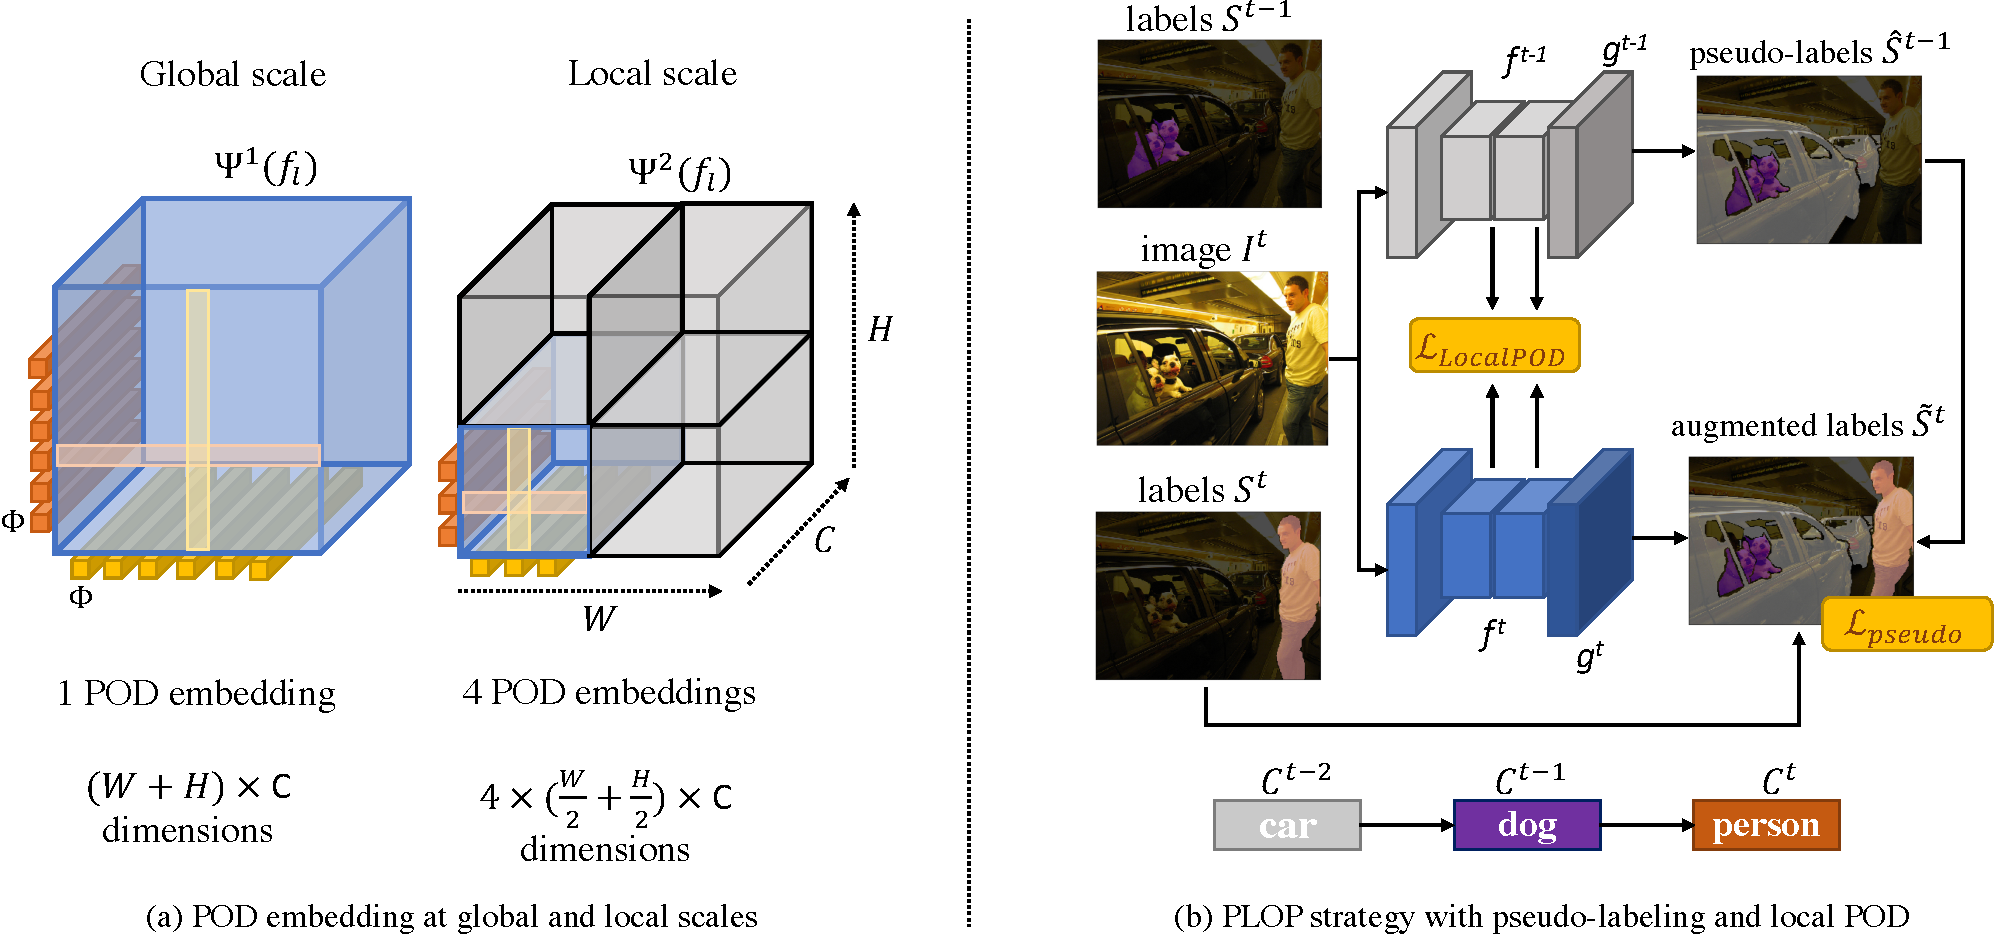
\includegraphics[width=\linewidth]{images/seg/plop_strategy.pdf}
    \caption{Local POD details and the complete PLOP strategy. (a) Local POD consists in POD
        embeddings compute at multiple scale. The global scale aggregates statistics across the
        whole features maps while the local scale focuses on finer details.  (b) The model
        incrementally learns new classes (\eg \texttt{car}, \texttt{dog},
        \texttt{person}). Only the current class (\texttt{person}) is labeled while previous classes
        are folded into the background. We use the previous model $g^{t-1} \circ f^{t-1}$ to
        generate pseudo-labels $\hat{\mcS}^{t-1}$ regarding the old classes to alleviate this
        ambiguity, and complete the labels $\mcS^t$ which are then used as ground-truth in
        $\mcL_\text{pseudo}$. The Local POD distillation is applied at multiple levels of the
        features extractors $f^{t-1}$ and $f^t$.}
    \label{fig:seg_model_plop}
\end{figure}

The model description is organized as follows: we first detail the continual protocol and the
notations. Then, we tackle the issue of catastrophic forgetting by designing an adapted distillation
loss, and we alleviate the background shift by proposing an uncertainty-based pseudo-labeling. Drawing
ideas from the continual learning literature, we propose an extension of PLOP specialized for
long-range continual training that we nickname PLOPLong. Finally, we detail the limits of rehearsal
learning in segmentation, propose a naive adaptation to the problem, and then deliver our carefully
designed method.

\subsection{Framework and notations}\label{sec:seg_overview}

For the notations, please refer to the \hyperref[chap:notations]{Notations}. The slight difference with
previous chapters, is that instead of working on pair of a classification image with a single label $(\vx,
    y)$, we will work on pairs of image and segmentation maps where each pixel has a class $(\vx^t,
    \vy^t)$. Here, the task identifier $t$ is even more important because the segmentation map $\vy$,
for a same image, will evolve through the tasks. Indeed, in the considered benchmarks (detailed
later in \autoref{sec:seg_exp}), an image is only labeled for the current classes $\vy^t$. The
previous $\mcC^{1:t-1}$ or future classes $\mcC^{t+1:T}$ the image may contain are not labeled, and
considered as the special class ``\textit{background}''. However, at test-time, a model at step $t$
must be able to discriminate between all the classes that have been seen so far, \textit{i.e.}
$\mcC^{1:t}$.

This leads us to identify two major pitfalls in \ac{CSS}: the first one, inherited from continual
learning, is catastrophic forgetting \cite{robins1995catastrophicforgetting}. It suggests that a
network will completely forget the old classes $\mcC^{1:t-1}$ when learning the new ones $\mcC^t$.

Furthermore, catastrophic forgetting is aggravated by the second pitfall, specific to \ac{CSS}, that
we call background shift: at step $t$, the pixels labeled as background are indeed ambiguous, as
they may contain either old (including the real background class, predicted in $\mcC^{1}$) or future
classes.

We define our model at step $t$ as a composition of a feature extractor $f^t(\cdot)$ (a ResNet 101
\cite{he2016resnet} backbone and a classifier $g^t(\cdot)$. The output predicted segmentation map
can then be written $\hat{\vy}^t = g^t \circ f^t(\vx)$. We denote the intermediate features at
each layer of the feature extractor $\vh_l^t = f_l^t(\cdot)\,,\, l \in \{1, \dots L\}$. Finally, we denote the
set of learnable parameters of $f^t$ and $g^t$ as $\Theta^t$.


\subsection{Overcoming catastrophic forgetting in CSS with local
    distillation}\label{sec:seg_distillation}

In this section, we propose to tackle the issue of catastrophic forgetting in continual learning in
general and in \ac{CSS} in particular. An effective method for doing so involves setting constraints
between the old ($g^{t-1} \circ f^{t-1}$) and current ($g^{t} \circ f^{t}$) models. These
constraints aim at enforcing a similar behavior between both models and in turn reduce the loss of
performance on old classes. A common such constraint is based on applying knowledge distillation
\cite{hinton2015knowledge_distillation,li2018lwf} between the predicted probabilities of both
models. When applied to \ac{CSS}, such distillation loss must be carefully balanced to find a good
trade-off between rigidity (\textit{i.e.} too strong constraints, resulting in not being able to
learn new classes) and plasticity (\textit{i.e.} enforcing loose constraints, which can lead to
catastrophic forgetting of the old classes).

In \autoref{chapter:regularization}, more precisely in \autoref{sec:podnet}, we designed POD, short
for Pooled Output Distillation. Rather than solely constraining the output model probabilities, POD
enforces consistency between intermediary statistics of both models. Recall
(\autoref{eq:podnet_pod_spatial}), for a feature map $\vx$, we define a POD embedding $\Phi(\cdot)$
as:
%
\begin{equation}
    \Phi(\vx) = \left[\frac{1}{W} \sum_{w=1}^W \vx[:,w,:] \bigg\Vert \frac{1}{H} \sum_{h=1}^H \vx[:,:,h]\right] \in \mathbb{R}^{(H + W) \times C}\,,
    \label{eq:seg_pod_embedding}
\end{equation}
%
where $[\cdot\,\|\,\cdot]$ denotes concatenation over the channel axis. The POD embedding is thus
computed as the concatenation of the $H \times C$ width-pooled slices and the $W \times C$
height-pooled slices of $\vx$ and captures long-range statistics across the whole features maps. The
POD distillation loss then consists in minimizing the $\mathcal{L}_2$ distance between POD
embeddings computed at several layers $l \in \{1, \dots, L\}$, w.r.t the current model parameters
$\Theta^t$:
%
\begin{equation}
    \mcL_\text{pod}(\Theta^t) = \frac{1}{L} \sum_{l = 1}^L \left\Vert  \Phi(\vh^t_l) -  \Phi(\vh^{t-1}_l) \right\Vert^2\,.
    \label{eq:seg_pod_loss}
\end{equation}
%
POD yielded state-of-the-art results in continual learning for image classification, especially when
large numbers of tasks are considered, a case where the aforementioned plasticity-rigidity trade-off
becomes even more crucial. Another interest arises in the context of \ac{CSS}: the long-range statistics
computed across an entire axis (horizontal or vertical) which reminds concurrent work on attention for
segmentation \citep{wang2020axialdeeplab,huang2020ccnet,park2020csc} which aim to enlarge the
receptive field through global attention/statistics \citep{wang2020axialdeeplab}. In the frame of
classification, it is, to a certain extent, necessary to discard spatial information through global
pooling. However, semantic segmentation requires the preservation of both long-range and
short-range statistics, making a distillation loss such as POD suboptimal for that purpose.


Following this reflection, and inspired by the multi-scale literature
\citep{lazbnik2006spatial_pyramid_matching,he2014spatialpyramidpooling}, we design a distillation
loss, called Local POD retaining the long-range spatial statistics while also preserving the local
information. The proposed Local POD consists in computing the width and height statistics at
different scales $\{1/2^s\}_{s=0 \dots S}$, as illustrated in \autoref{fig:seg_model_plop} (a). At a
given level $l$ of the feature extractor, $s^2$ POD embeddings are computed per scale $s$ and
concatenated:
%
\begin{equation}
    \Psi^s(\vx) = \left[ \Phi(\vx^s_{1,1}) \| \dots \| \Phi(\vx^s_{s,s}) \right] \in \mathbb{R}^{\times (H + W) \times C}\,,
    \label{eq:seg_localpod_embedding1}
\end{equation}
%
where $\forall i = 1 \dots s$, $\forall j = 1 \dots s$, $\vx^s_{i,j} = \vx[:, i W/s:(i+1) W/s, j
        H/s:(j+1) H/s]$ is a sub-region of the embedding tensor $\vx$ of size $W/s \times H/s$.
Then, we concatenate (along the channel axis) the Local POD embeddings $\Psi^s(\vx)$ of each
scale $s$ to form the final embedding:
%
\begin{equation}
    \Psi(\vx) = \left[ \Psi^1(\vx) \| \dots \| \Psi^S(\vx) \right] \in \mathbb{R}^{S \times (H + W) \times C}\,.
    \label{eq:seg_local_pod}
\end{equation}
%
Similarly to POD, we compute Local POD embeddings for every layer $l \in \{1, \dots, L\}$ of both
the old and current models. The resulting loss is thus:
%
\begin{equation}
    \mcL_{\scriptstyle\text{LocalPod}}(\Theta^t) = \frac{1}{L} \sum_{l = 1}^L \left\Vert  {\Psi}(f^t_l(I)) -  {\Psi}(f^{t-1}_l(I)) \right\Vert^2\,.
    \label{eq:seg_local_pod_loss}
\end{equation}
%
Thus, notice that the first scale of Local POD ($1/2^0$) is similar to the original POD and models
long-range dependencies across the entire image. The subsequent scales ($s=1/2^1, 1/2^2 \dots$),
enforce short-range dependencies. Thus, the proposed Local POD tackles the problem of catastrophic
forgetting by modeling and preserving long and short-range statistics between the old and current
models, throughout the \ac{CSS} steps.


\subsection{Pseudo-labeling to fix background shift}\label{sec:seg_hardpl}

In addition to catastrophic forgetting, a successful \ac{CSS} approach shall handle the background shift
problem, thus shall take into account the ambiguity of pixels labeled as background at each step.
We propose a pseudo-labeling strategy that ``\textit{completes}'' the ambiguous background labels.
Pseudo-labeling \citep{lee2013pseudolabel} is commonly used in domain adaption for semantic
segmentation
\citep{vu2019advent,li2019bidirectionallearning,zou2018classbalancedselftraining,saporta2020esl}
where a model is trained to match both the labels of a source dataset and the pseudo-labels (usually
obtained using the same predictive model, in a self-training fashion) of an unlabeled target
dataset. In this case, the knowledge acquired on the source dataset helps the model to generate
labels for the target dataset. In the frame of \ac{CSS}, at each step, we use the predictions of the old
model to decipher previously seen classes among the ambiguous background pixels, as illustrated in
\autoref{fig:seg_model_plop}. The pseudo-labeling relies on the previous model which can be uncertain
for some pixels due to inherent bias to the optimization and because of the forgetting. Therefore,
in order to avoid propagating errors through incorrect pseudo-labels, we filter out the most uncertain
ones based on an adaptive entropy-based threshold.

Formally, let $\mcN^t=\operatorname{card}(\mcC^{t})$ the cardinality of the current classes,
excluding the background class. Let $\hat{\vy}^{t} \in \mathbb{R}^{W,H,1+\mcN^{1:t}}$ denotes the
predictions of the current model (which includes the real background class, all the old classes as
well as the current ones). We define $\tilde{\vy}^{t} \in \mathbb{R}^{W,H,1+\mcN^{1:t}}$ the target
as step $t$, computed using the one-hot ground-truth segmentation map $\vy^{t} \in
    \mathbb{N}^{W,H,1+\mcN^t}$ at step $t$ as well as pseudo-labels extracted using the old model
predictions $\hat{\vy}^{t-1} \in \mathbb{R}^{W,H,1+\mcN^{1:t-1}}$ as follows:
%
\begin{equation}
    \footnotesize
    \tilde \mcS^{t}\left(w,h,c\right)= \mkern-5mu \left\{\begin{array}{ll}
        \mkern-10mu 1 \mkern-27mu & \text { if } \vy^{t} [c_{bg},w,h]=0 \text { and } c = \argmax \limits_{c' \in \mcC^{t}} \vy^{t}[c',w,h])                                 \\
        \mkern-10mu 1 \mkern-27mu & \text { if } \vy^{t}[c_{bg},w,h]=1 \text { and } c = \mkern-8mu \argmax \limits_{c' \in \mcC^{1:t-1}} \mkern-6mu \hat{\vy}^{t-1}[c',w,h] \\
        \mkern-10mu 0 \mkern-27mu & \text { otherwise }                                                                                                                      \\
    \end{array}\right.
    \label{eq:seg_pseudo_bis}
\end{equation}
%
In other words, in the case of non-background pixels we simply copy the ground truth label.
Otherwise, we use the class predicted by the old model $g^{t-1}(f^{t-1}(\cdot))$. This pseudo-label
strategy allows assigning each pixel labeled as background his real semantic label if this pixel
belongs to any of the old classes. However, pseudo-labeling all background pixels can be
unproductive, \eg on uncertain pixels where the old model is likely to fail. Therefore, we only keep
pseudo-labels where the old model is deemed ``\textit{confident}'' enough.
\autoref{eq:seg_pseudo_bis} is modified to take into account this uncertainty:
%
\begin{equation}
    \scriptsize
    \tilde \mcS^{t}\left(w,h,c\right)\mkern-5mu = \mkern-5mu \left\{\begin{array}{ll}
        \mkern-14mu 1 \mkern-27mu & \mkern-8mu \text { if } \vy^{t} \mkern-4mu [c_{bg},w,h]\mkern-4mu = \mkern-4mu 0 \text { and } c \mkern-4mu = \mkern-4mu \argmax \limits_{c' \in \mcC^{t}} \vy^{t} \mkern-4mu [c',w,h]                                                                          \\
        \mkern-14mu 1 \mkern-27mu & \mkern-8mu \text { if } \vy^{t} \mkern-4mu [c_{bg},w,h] \mkern-4mu = \mkern-4mu 1 \text { and } c \mkern-4mu = \mkern-12mu \argmax \limits_{c' \in \mcC^{1:t-1}} \mkern-6mu \hat \vy^{t-1} \mkern-4mu [c',w,h]  \text{ and } u \mkern-4mu < \mkern-4mu \tau_{c} \\
        \mkern-14mu 0 \mkern-27mu & \mkern-4mu \,\text { otherwise\,, }                                                                                                                                                                                                                             \\
    \end{array}\right.
    \label{eq:seg_pseudo_bis_uncertain}
\end{equation}
%
By notation abuse, $u$ is function $u(\vy^t(w, h))$ that measures the uncertainty of the current
model given a pixel $\vx[:,w,h]$. $\tau_{c}$ denotes a class-specific uncertainty threshold. Hence,
in the case where the old model is uncertain ($u \ge \tau_c$) about some pixels, they will be
ignored in the final classification loss. Our framework is agnostic to the type of uncertainty used,
but in practice we define it as the entropy. Therefore, we use for $u$ the current model's per-pixel
entropy $u(\vy^t[:,w, h]) = -\sum_{c \in C^{1:t}} \vy^t[c,w, h] \log \vy^t[c,w, h]$. Likewise,
the class-specific threshold $\tau_c$ is computed from the median entropy of the old model over all
pixels of $\mcD^t$ predicted the class $c$ for all $c \in \mcC^{1:t-1}$ as proposed by
\cite{saporta2020esl}. Consequently, the cross-entropy loss with pseudo-labeling of the old classes
can be written as:
%
\begin{equation}
    \mcL_\text{pseudo}(\Theta^t)=- \frac{\nu}{WH} \sum_{w,h}^{W,H} \sum_{c \in \mcC^{t}} \tilde \vy\left(w,h,c\right) \log \hat \vy^{t}\left[c,w,h]\right)\,.
    \label{eq:seg_pseudo_loss}
\end{equation}
%
We reduce the normalization factor $WH$ proportionally to the number of discarded pixels. To avoid
giving disproportional importance to the pixels belonging to new classes (which are not discarded),
we introduce in \autoref{eq:seg_pseudo_loss} an adaptive factor $\nu$, which is the ratio of
accepted old classes pixels over the total number of such pixels. \textit{i.e.} if most of the image
is uncertain, the overall importance of the image relative to other images in the batch is reduced.
The overall behavior of our pseudo-labeling is illustrated in \autoref{fig:seg_model_plop}.

We call our final model PLOP (standing for Pseudo-labeling and LOcal Pod). PLOP's final loss is a
weighted combination of \autoref{eq:seg_local_pod_loss} and \autoref{eq:seg_pseudo_loss}:
%
\begin{equation}
    \mcL(\Theta^t) = \underbrace{\strut \mcL_\text{pseudo}(\Theta^t)}_\text{classification} + \lambda\underbrace{\strut \mcL_\text{localPod}(\Theta^t)}_\text{distillation}\,,
    \label{eq:seg_complete_loss}
\end{equation}
%
\noindent with $\lambda$ a hyperparameter. PLOP, while already very competitive, can face difficulties when
dealing with long continual settings, \textit{i.e.} for which the number of steps grows larger. For
this reason, we propose PLOPLong, an extension of PLOP for dealing with such cases.

\subsection{PLOPLong: a specialization for long settings}\label{sec:seg_plopv2}

While the proposed method already achieves satisfying results in traditional \ac{CSS} scenarios, it might
struggle to deal with longer settings due to two major drawbacks, namely specialization of the
classifier towards the recent classes, and the shifts of the batch normalization layers.

First, we observe that in \ac{CSS} the classifier weights tend to be specialized for the last classes to
the detriment of older classes \citep{hou2019ucir}. Several solutions exist that aim at correcting
this bias
\citep{wu2019bias_correction,belouadah2019il2m,zhao2020weightalignement,luo2018cosine_classifier}, and
we choose the cosine normalization. In practice, we replace the classifier with a cosine classifier
\citep{luo2018cosine_classifier}, where the final inner product is discarded in favor of cosine
similarity. By doing so, all class weights --both old and new-- have a constant magnitude of 1,
which drastically reduces the bias towards new classes. The classifier $g^t$ is in segmentation a
pointwise ($1\times1$ kernel) convolution which does not alter the spatial organization but maps the
$ch$ features channels to $\mcC^{1:t}$ channels, one per class to predict. This pointwise
convolution can be seen as a fully-connected layer that is applied independently to each pixel.
Therefore, the classifier $g^t$ has $\{\theta_c^t \in \mathbb{R}^{ch} | \forall c \in \mcC^{1:t}\}$.
The cosine normalization can then be expressed as:
%
\begin{equation}
    \hat{\mcS}(w, h, c) = \frac{\alpha \langle \theta^t_c, \vh(w, h) \rangle}{\Vert \theta^t_c \Vert^2 \Vert \vh[:,w, h] \Vert^2}\,
    \label{eq:seg_cosine_classifier}
\end{equation}
%
\noindent with $\alpha$ a learned scalar parameter initialized to 1 and helping the convergence, and $\vh \in
    \mathbb{R}^{W \times H \times ch}$ the final features embedding before the classifier. First
used in continual learning by \cite{hou2019ucir}, this classifier has more recently be adopted
by continual few-shot segmentation \citep{cermelli2020fewshotcontinualsegm} or multi-modes
continual learning \citep{douillard2020podnet}. The new cosine classifier weights that
correspond to the new classifier can then be initialized with weight imprinting
\citep{qi2018imprintedweights} as recently adapted for segmentation by
\cite{cermelli2020fewshotcontinualsegm}.

Furthermore, we propose to exploit the cosine normalization for intermediary features: the
comparison between the Local POD embeddings of the previous model $f^{t-1}$ with the current $f^t$
can be too constrained. We relax the constraints by imposing not a low Euclidean distance between
both embeddings, but rather a high cosine similarity, which allows us better plasticity to learn new
classes. We need to alter \autoref{eq:seg_local_pod_loss} by replacing the $\Phi(\cdot)$ operator by
$\bar{\Phi}(\cdot) = \nicefrac{\Phi(\cdot)}{\vert\Phi(\cdot)\Vert^2}$. However, note that the
features from level $l$ given to level $l+1$ are not normalized. The normalization only happens for
the Local POD embeddings.

Second, an almost ubiquitous component of modern deep computer vision models is the Batch
Normalization \citep{ioffe2015batchnorm}. It normalizes internal representation with the batch mean
$\mu_\mathbb{B}$ and batch standard deviation $\sigma_\mathbb{B}$ (resp. running mean $\mu$ and
running std $\sigma$) during training (resp. testing). Formally for a batch normalization layer
taking an input $\vx$ and producing an output $\vy$:
%
\begin{equation}
    \vy = \frac{\vx - \mu_\mathbb{B}}{\sigma_\mathbb{B}} \cdot \gamma + \beta
    \label{eq:seg_batch_norm}
\end{equation}
%
with $\gamma$ and $\beta$ two learned parameters. The important drawback of this normalization layer
is its assumption that the data is sampled \textit{i.i.d.} which is not the case in continual
segmentation where multiple shifts
\citep{morenotorresa2012datasetshift,lesort2021driftanalysis,douillardlesort2021continuum}, happen in
the training tasks, different from the testing tasks. Drawing inspiration from the domain
incremental \citep{lomonaco2020ar1} and continual few-shots segmentation
\citep{cermelli2020fewshotcontinualsegm} literature, we choose to replace the batch normalization by
batch \textit{re}normalization \citep{ioffe2017batchrenorm}, i.e.:
%
\begin{equation}
    \vy = \frac{\vx - \mu_\mathbb{B}}{\sigma_\mathbb{B}} \cdot r + d,\,\text{where}\, r = \frac{\sigma_\mathbb{B}}{\sigma},\, d = \frac{\mu_\mathbb{B} - \mu}{\sigma}\,.
    \label{eq:seg_batch_renorm}
\end{equation}
%
Intuitively, batch renormalization avoids the discrepancy between training and testing of the batch
normalization. Furthermore, following \cite{cermelli2020fewshotcontinualsegm}, we freeze during
training the statistics ($\mu$ and $\sigma$) after the first task to avoid harmful statistics
drifts.

All these improvements further increase performance for long series of tasks: (1) Cosine classifier
reduces the increased bias between recent and old classes. (2) A cosine-based Local POD relax the
constraints in order to correctly learn the bigger number of new classes. (3) Frozen BatchReNorm
reduces the inherent drift of statistics that grow larger as the number of tasks increases. In what
follows, we denote PLOPLong the model obtained from PLOP by adding all three improvements. We
empirically saw that these contributions marginally improve PLOP taken individually, but when used
altogether provided an major boost of performance in long-range scenarios.


\begin{figure*}[ht!]
    \centering
    \includegraphics[width=\linewidth]{images/seg/rehearsal_strategy.pdf}
    \caption{\textbf{Our Object Rehearsal strategy}. In task $t-1$, we select from $\{\vx^{t-1},
            \dots \}$ a limited amount of objects (here \texttt{bus}, \texttt{bird}, and
        \texttt{dog}), which will be then mixed in the images $\{\vx^{t}, \dots \}$ from the
        current task $t$; after pasting, the other present objects are erased. Finally, the
        current model $g^t \circ f^t$ will be given the concatenation of the original images
        and the augmented images $\{\vx''^t, \dots\}$. Our Object Rehearsal allows to generate
        a wider diversity of images, resulting in higher accuracies while being up to 146x more
        memory efficient.}
    \label{fig:seg_model_objectrehearsal}
\end{figure*}


\section{Object Rehearsal}
\label{sec:seg_rehearsal}

Neither the proposed PLOP nor PLOPLong did make use of previously seen data $\{\mcD^{1}, \dots,
    \mcD^{t-1}\}$ when considering step $t$. In this section, we explore how to further improve \ac{CSS}
performance if a model is now allowed to rehearse a limited amount of previous data. We first
consider a traditional approach, namely Image Rehearsal. We show that such a naive approach
cannot work well in the frame of \ac{CSS} and propose innovative adaptations to make it work. Then,
we highlight the drawbacks of this rehearsal method and propose a novel approach named Object
Rehearsal, more effective both in terms of \ac{mIoU} and memory consumption.

\subsection{Image Rehearsal}
\label{sec:seg_image_rehearsal}

We first consider rehearsing a limited amount of images from previous tasks during the current task.
Image rehearsal is a well-studied problem in continual image classification. However, it was rarely
applied to other tasks. Contrary to image classification, in \ac{CSS}, images can have multiple labels if
several objects (\eg \texttt{car}, \texttt{sky}) are present in the image. Moreover, as we
described previously in \autoref{sec:seg_overview}, the segmentation maps are partially labelized. For a
given task $t$, when rehearsing an image stored from task $t-i$, we only have labels of classes
$C^{t-1}$. Because of these two problems, we cannot naively apply image rehearsal on \ac{CSS}. To tackle
the former problem, we propose to select $M$ images for each class $c \in C^t$, resulting in $M
    \times \mcN^t$ images for step $t$. We ensure that the selected images are unique: as multiple
classes can co-exist in the same image, the resulting amount of sampled classes may be above $M
    \times \mcN^t$. We select the images with a simple random selection, which has been proved to
generally perform as good as more elaborate methods \citep{castro2018end_to_end_inc_learn}. The
memory footprint will grow until all tasks but the last are seen, resulting in a total amount of $M
    \times \mcN^{1:T-1}$ stored images. To address the second problem (partial labelization, see also
Section \ref{sec:seg_hardpl}), we fill the background using our proposed hard pseudo-labeling (see
\autoref{sec:seg_hardpl}) which \textit{completes} the segmentation maps with old classes
$\mcC^{1:t-i}$ as well as new classes $\mcC^{t-i+1:t}$.

\subsection{Object Rehearsal}
\label{sec:seg_object_rehearsal}

The main drawback of image rehearsal is that \ac{CSS} images are usually large (from $512\times 512$ to
$1024 \times 2048$) yet they are sparsely informative, as a significant part of the images consists
in background pixels \citep{lin2017focalloss} (\eg 63\% of Pascal-VOC \citep{everingham2015pascalvoc}
pixels) or belongs to a majority class (\eg 32\% of Cityscapes \citep{cordts2016cityscapes} pixels
are \texttt{roads}).

To address both problems, instead of storing whole images from the previous tasks $\{1, ..., t-1\}$,
we propose to store an informative portion that we will mix with the images of the current task $t$.
Image mixing is popular for classification
\citep{hingyi2018mixup,yun2019cutmix,dabouei2020supermix,verma2019manifoldmixup,li2021moex,rame2021mixmo}
yet, to the best of our knowledge, sees limited use for semantic segmentation
\citep{fang2019instaboost,olsson2021classmix,zhang2021objectaug,tranheden2021dacs,ghiasi2020simplecopypaste},
and has never been considered to design memory-efficient rehearsal learning systems. Formally, given
an image $\vx$ and the corresponding ground truth segmentation maps $\vy^t$, we define a binary mask
$\Pi_c$  such that $\forall c \in \mcC^t$:
%
\begin{equation}
    O_c = I \odot \Pi_c\,\text{where}\,\Pi[:, w, h] = \left\{\begin{array}{l}
        1, \text{if} \vy^t[:,w, h] = c \\
        0, \text{otherwise}
    \end{array}\right.\,,
    \label{eq:seg_mask_object}
\end{equation}
%
\noindent with $O_c$ the selected object for class $c$. By nature, this patch is extremely sparse
and can be efficiently stored on disk by modern compression algorithms \citep{ISO)10918}. The total
memory footprint at task t is thus $M \times \mcN^{1:t}$ objects.

Then, when learning a task $t > 1$, the model will learn on both the task dataset $\cup_i^N
    (\vx^t_i, \vy^t_i)$ and the object memory $\cup_{c \in \mcC^{1:t-1}} \cup_i^M O_{c,i}$, with $N$
being the total number of images in the task dataset. The latter will augment the former through
object pasting. We augment each object by applying an affine transformation matrix
\citep{fang2019instaboost}:
%
\begin{equation}
    \mathbf{T}=\left[\begin{array}{ccc}
            z \cos \alpha  & z \sin \alpha & 0 \\
            -z \sin \alpha & z \cos \alpha & 0 \\
            0              & 0             & 1
        \end{array}\right]\,,
    \label{eq:seg_transformation_matrix_complex}
\end{equation}
%
\noindent with $z$ a zoom factor, and $\alpha$ an in-plane rotation angle. Note that we do not
translate the object as its original position is often a good prior: indeed, objects are usually
located at the same location (\eg pedestrian on the left and right sidewalk, car on the middle
road, etc.) We abuse the notation by denoting $T(.)$ the application of this transformation matrix.
Once the data augmentation is done on the object (and its mask), we paste it on an image $\vx^t$ that
refers to the current task:
%
\begin{equation}
    {\vx'}^t = \vx^t \odot (\mathbf{1} - T(\Pi_c)) + T(O_c) \odot T(\Pi_c)\,.
    \label{eq:seg_pasting}
\end{equation}
%
The pasting can result in local incoherence where the pixel of a \texttt{cow} is pasted on top or
next to the pixel of a \texttt{television}. Naively the object borders can be smoothed into the
image with a Gaussian filter. Unfortunately, it results in imprecise contours, which are important in
segmentation \citep{chen2020semeda}.

This approach has already been envisioned as a form of data augmentation in semantic segmentation,
although the gains were small and to avoid the noise induced by this pasting, the batch size is
prohibitively large (up to 512) \citep{ghiasi2020simplecopypaste}. We propose to reduce interference
between the pasted object and the destination images by \textbf{selective erasing} of the
surrounding pixels. Indeed, given a binary matrix $\Xi(\Pi, S)$ of the same dimension as $I$ and
$\Pi$:
%
\begin{equation}
    {\vx''}^t = {\vx'}^t \odot (\mathbf{1} - \Xi) + \kappa \odot \Xi\,.
    \label{eq:seg_erasing_pixel}
\end{equation}
%
We replace the pixels erased according to the mask $\Xi$ with a RGB color $\kappa \in \mathbb{R}^3$.
This RGB vector could be chosen through in-painting \citep{fang2019instaboost} or be random noise,
but in practice, we choose a constant color gray. We also update the segmentation maps accordingly:
%
\begin{equation}
    {\vy''}^t = {\y'}^t \odot (\mathbf{1} - \Xi) + 255 \odot \Xi\,,
    \label{eq:seg_erasing_label}
\end{equation}
%
\noindent where \texttt{255} is a dummy class id used in segmentation to ignore some pixel labels
which will not be counted in the classification loss \autoref{eq:seg_pseudo_loss}. We illustrate our
rehearsal strategy in \autoref{fig:seg_model_objectrehearsal}.

\begin{table}[t]
    \centering
    \caption{Description of the three datasets considered in this paper. For datasets without explicit background class, one is created based on unlabeled pixels.}
    \vspace*{-0.3cm}
    \label{tab:dataset_description}
    \begin{tabular}{@{}l|ccccc@{}}
        \toprule
        Dataset                                   & \# classes & {\scriptsize Background?} & \# train & \# test & {\scriptsize Image size} \\
        \midrule
        Pascal-VOC \cite{everingham2015pascalvoc} & 20         & \cmark                    & 10k      & 1.5k    & $512 \times 512$         \\
        Cityscapes \cite{cordts2016cityscapes}    & 19         & \xmark                    & 3k       & 0.5k    & $512 \times 1024$        \\
        ADE20k \cite{zhou2017adedataset}          & 150        & \xmark                    & 20k      & 2.0k    & $512 \times 512$         \\
        \bottomrule
    \end{tabular}
\end{table}

\begin{table}[t]
    \centering
    \caption{Description of the 12 different benchmarks evaluated in this paper. For some of these, each task brings new classes while, for others, it comes with new domains.}
    \vspace*{-0.3cm}
    \label{tab:setting_description}
    \begin{tabular}{@{}l|rcccc@{}}
        \toprule
        {\scriptsize Dataset}       & {\scriptsize Setting} & {\scriptsize Mode} & {\scriptsize \# tasks} & {\scriptsize \# base classes} & {\scriptsize \# classes / inc. task} \\
        \midrule
        \multirow{4}{*}{Pascal-VOC} & 19-1                  & class              & 2                      & 19                            & 1                                    \\
                                    & 15-5                  & class              & 2                      & 15                            & 5                                    \\
                                    & 15-1                  & class              & 6                      & 15                            & 1                                    \\
                                    & 10-1                  & class              & 11                     & 10                            & 1                                    \\
        \hline
        \multirow{1}{*}{Cityscapes} & 14-1                  & class              & 6                      & 14                            & 1                                    \\
        %& 11-5 & domain  & 3 & 11 & 5 \\
        %& 11-1 & domain  & 11 & 11 & 1 \\
        %& 1-1 & domain  & 21 & 1 & 1 \\
        \hline
        \multirow{4}{*}{ADE20k}     & 100-50                & class              & 2                      & 100                           & 50                                   \\
                                    & 50-50                 & class              & 2                      & 50                            & 50                                   \\
                                    & 100-10                & class              & 6                      & 100                           & 10                                   \\
                                    & 100-5                 & class              & 11                     & 100                           & 5                                    \\
        \bottomrule
    \end{tabular}
\end{table}


\begin{figure}
    \centering
    \includegraphics[width=0.5\linewidth]{images/seg/dataset_viz.pdf}
    %\vspace*{-0.3cm}
    \caption{\textbf{Dataset visualization:} of an example image and its segmentation maps for Pascal-VOC, ADE20k, and Cityscapes.}
    \label{fig:seg_dataset_viz}
\end{figure}

\section{Experiments}
\label{sec:seg_exp}

\subsection{Datasets, Protocols, and Baselines}
\label{sec:seg_datasets_protocols}

To ensure fair comparisons with state-of-the-art approaches, we follow the experimental setup of
~\cite{cermelli2020modelingthebackground} for datasets, protocol, metrics, and baseline
implementations. Although, we also propose to evaluate on new datasets and on more challenging
protocols. Furthermore, we explore in advanced experiments, for the first time, how rehearsal can
improve performance in \ac{CSS}.

\paragraph{Datasets:} We evaluate our model on three datasets, summarized in
\autoref{tab:seg_dataset_description}: Pascal-VOC \citep{everingham2015pascalvoc},
Cityscapes \citep{cordts2016cityscapes} and ADE20k \citep{zhou2017adedataset}. VOC contains 20
classes, 10,582 training images, and 1,449 testing images. Cityscapes contains 2975 and 500 images
for train and test, respectively. Those images represent 19 classes and were taken from 21 different
cities. ADE20k has 150 classes, 20,210 training images, and 2,000 testing images. All ablations and
hyperparameters tuning were done on a validation subset of the training set made of 20\% of the
images. For all datasets, we use random resize and crop augmentation (scale from 80\% to 110\%), as
well as random horizontal flip during training time. The final image size for Pascal-VOC and ADE20k
is $512 \times 512$ while it is $512 \times 1024$ for Cityscapes.

\paragraph{CSS protocols:} \cite{cermelli2020modelingthebackground} introduced the
\textit{Overlapped} setting where only the current classes are labeled \vs a background class
$\mcC^t$. Moreover, pixels can belong to any classes $\mcC^{1:t-1} \cup \mcC^{t} \cup \mcC^{t+1:T}$
(old, current, and future). Those two constraints make this setting both challenging and realistic,
as in a real setting there is not any oracle method to exclude future classes from the background. In
all our experiments, we respect the Overlapped setting. While the training images are only labeled
for the current classes, the testing images are labeled for all seen classes. We evaluate several
\ac{CSS} protocols for each dataset, \eg on VOC 19-1, 15-5, and 15-1 respectively consists in learning
19 then 1 class ($T=2$ steps), 15 then 5 classes ($2$ steps), and 15 classes followed by five times
1 class ($6$ steps). The last setting is the most challenging due to its higher number of steps.
Similarly, on Cityscapes 14-1 means 14 followed by five times 1 class ($6$ steps) and on ADE 100-50
means 100 followed by 50 classes ($2$ steps). We provide a summary of all these settings in
\autoref{tab:seg_setting_description}.

\paragraph{Metrics:} In \autoref{sec:related_metrics}, we defined the \textbf{final} and
\textbf{average} incremental accuracies. In the context of semantic segmentation, we generalize
those metrics to the \acf{mIoU}. Specifically, we compute \ac{mIoU} after the last step $T$ for the
initial classes $\mcC^{1}$, for the incremented classes $\mcC^{2:T}$, and for all classes
$\mcC^{1:T}$ (\textit{final}). These metrics respectively reflect the robustness to catastrophic
forgetting (the model rigidity), the capacity to learn new classes (plasticity), as well as its
overall performance (trade-of between both). We also introduce the \textit{avg} metric (short for
\textit{average}), novel in \ac{CSS}, which measures the average of \ac{mIoU} scores measured step
after step, integrating performance over the whole continual learning process. We stress that all
four metrics are important, and we should not disregard one for the other: a model suffering no
forgetting but not able to learn anything new is useless.

\paragraph{Baselines:} We benchmark our model against the latest state-of-the-arts \ac{CSS}
methods ILT \citep{michieli2019ilt}, MiB \citep{cermelli2020modelingthebackground}, GIFS
\citep{cermelli2020fewshotcontinualsegm}, and SDR \citep{michieli2021sdr}. Note that while GIFS was
created by \cite{cermelli2020fewshotcontinualsegm} for continual \textit{few-shots}
segmentation, we adapt it for the more general task of \ac{CSS}. Unless stated otherwise, all the results
are excerpted from the corresponding papers. We also evaluate general continual models based on
weight constraints (PI \citep{zenke2017synaptic_intelligence}, EWC \citep{kirkpatrick2017ewc}, and RW
\citep{chaudhry2018riemannien_walk}) and knowledge distillation (LwF \citep{li2018lwf} and LwF-MC
\citep{rebuffi2017icarl}). Moreover, unless explicitly stated otherwise, all the models (ours
included), do not use rehearsal learning.


\paragraph{Implementation Details:} As in \cite{cermelli2020modelingthebackground}, we use a
Deeplab-V3 \citep{chen2017deeplabv3} architecture with a ResNet-101 \citep{he2016resnet} backbone
pretrained on ImageNet \citep{deng2009imagenet} for all experiments and models but SDR
\citep{michieli2021sdr} which used a Deeplab-V3+ \citep{chen2018deeplabv3plus}. For all datasets, we
set a maximum threshold for the uncertainty measure of \autoref{eq:seg_pseudo_bis_uncertain} to
$\tau=1e-3$. We train our model for 30, 60, and 30 epochs per \ac{CSS} step on Pascal-VOC, ADE20k, and
Cityscapes, respectively, with an initial learning rate of $1e-2$ for the first \ac{CSS} step, and $1e-3$
for all the following ones. Note that for Cityscapes, the first step is longer with 50 epochs. We
reduce the learning rate exponentially with a decay rate of $9e-1$. We use SGD optimizer with $9e-1$
Nesterov momentum. The Local POD weighting hyperparameter $\lambda$ is set to $1e-2$ and $5e-4$ for
intermediate feature maps and logits, respectively. Moreover, we multiply this factor by the
adaptive weighting $\sqrt{\nicefrac{|C^{1:t}|}{|C^{t}|}}$ introduced by \citep{hou2019ucir} that
increases the strength of the distillation the further we are into the continual process. For all
feature maps, Local POD is applied before ReLU, with squared pixel values, as in
\cite{zagoruyko2016distillation_attention,douillard2020podnet}. We use 3 scales for Local POD: $1$,
$\nicefrac{1}{2}$, and $\nicefrac{1}{4}$, as adding more scales experimentally brought diminishing
returns. For PLOPLong only, we L2-normalize all POD embeddings before distilling them as also done
by \cite{douillard2020podnet}. Furthermore, for PLOPLong, the gradient norm-clipping is set at $1.0$
for Pascal-VOC and $2.0$ for Cityscapes. We use a batch size of 24 distributed on two 12Go Titan Xp
GPUs. Contrary to many continual models, we do not have access to any task id in inference, therefore
our setting/strategy has to predict a class among the set of all seen classes



\subsection{PLOP and PLOPLong experiments}
\label{sec:seg_plop_exp}

\subsubsection{Quantitative Evaluations}


\begin{table*}[t]
    \centering
    \begin{adjustbox}{max width=\textwidth}
        \begin{tabular}{@{}l|cccc||cccc||cccc@{}}
            \toprule
                                                                           & \multicolumn{4}{c}{\textbf{19-1} (2 tasks)} & \multicolumn{4}{c}{\textbf{15-5} (2 tasks)} & \multicolumn{4}{c}{\textbf{15-1} (6 tasks)}                                                                                                                                                                         \\
            \textbf{Method}                                                & 0-19                                        & 20                                          & \textit{final}                              & \textit{avg}   & 0-15              & 16-20          & \textit{final}    & \textit{avg}   & 0-15              & 16-20             & \textit{final}    & \textit{avg}   \\
            \midrule
            % from paper MiB
            $\text{Fine Tuning}^\dagger$                                   & \tableindent 6.80                           & 12.90                                       & \tableindent 7.10                           &                & \tableindent 2.10 & 33.10          & \tableindent 9.80 &                & \tableindent 0.20 & \tableindent 1.80 & \tableindent 0.60 &                \\
            $\text{PI}^\dagger$ \citep{zenke2017synaptic_intelligence}     & \tableindent 7.50                           & 14.00                                       & \tableindent 7.80                           &                & \tableindent 1.60 & 33.30          & \tableindent 9.50 &                & \tableindent 0.00 & \tableindent 1.80 & \tableindent 0.50 &                \\
            $\text{EWC}^\dagger$ \citep{kirkpatrick2017ewc}                & 26.90                                       & 14.00                                       & 26.30                                       &                & 24.30             & 35.50          & 27.10             &                & \tableindent 0.30 & \tableindent 4.30 & \tableindent 1.30 &                \\
            $\text{RW}^\dagger$ \citep{chaudhry2018riemannien_walk}        & 23.30                                       & 14.20                                       & 22.90                                       &                & 16.60             & 34.90          & 21.20             &                & \tableindent 0.00 & \tableindent 5.20 & \tableindent 1.30 &                \\
            $\text{LwF}^\dagger$ \citep{li2018lwf}                         & 51.20                                       & \tableindent 8.50                           & 49.10                                       &                & 58.90             & 36.60          & 53.30             &                & \tableindent 1.00 & \tableindent 3.90 & \tableindent 1.80 &                \\
            $\text{LwF-MC}^\dagger$ \citep{rebuffi2017icarl}               & 64.40                                       & 13.30                                       & 61.90                                       &                & 58.10             & 35.00          & 52.30             &                & \tableindent 6.40 & \tableindent 8.40 & \tableindent 6.90 &                \\
            $\text{ILT}^\dagger$ \citep{michieli2019ilt}                   & 67.10                                       & 12.30                                       & 64.40                                       &                & 66.30             & 40.60          & 59.90             &                & \tableindent 4.90 & \tableindent 7.80 & \tableindent 5.70 &                \\
            $\text{ILT}$ \citep{michieli2019ilt}                           & 67.75                                       & 10.88                                       & 65.05                                       & 71.23          & 67.08             & 39.23          & 60.45             & 70.37          & \tableindent 8.75 & \tableindent 7.99 & \tableindent 8.56 & 40.16          \\

            $\text{MiB}^\dagger$ \citep{cermelli2020modelingthebackground} & 70.20                                       & 22.10                                       & 67.80                                       &                & 75.50             & 49.40          & 69.00             &                & 35.10             & 13.50             & 29.70             &                \\
            % from us
            MiB \citep{cermelli2020modelingthebackground}                  & 71.43                                       & 23.59                                       & 69.15                                       & 73.28          & \textbf{76.37}    & 49.97          & \textbf{70.08}    & \textbf{75.12} & 34.22             & 13.50             & 29.29             & 54.19          \\
            $\text{SDR}^\diamond$ \citep{michieli2021sdr}                  & 71.30                                       & 23.40                                       & 69.0                                        &                & 76.30             & 50.20          & 70.10             &                & 47.30             & 14.70             & 39.50             &                \\
            GIFS \citep{cermelli2020fewshotcontinualsegm}                  & 57.88                                       & 32.82                                       & 56.69                                       & 67.05          & 23.61             & 16.43          & 21.90             & 50.97          & 59.36             & 13.89             & 48.53             & 61.43          \\
            \hdashline
            PLOP                                                           & \textbf{75.35}                              & 37.35                                       & \textbf{73.54}                              & \textbf{75.47} & 75.73             & \textbf{51.71} & \textbf{70.09}    & \textbf{75.19} & 65.12             & 21.11             & 54.64             & 67.21          \\
            PLOPLong                                                       & 74.75                                       & \textbf{39.68}                              & 73.08                                       & 74.32          & 75.95             & 48.31          & 69.37             & 73.58          & \textbf{72.00}    & \textbf{26.66}    & \textbf{61.20}    & \textbf{70.02} \\
            %{\color{red}HRHF} \cite{huang2021halfrealhalffake} & 76.60 & 57.30 & 75.70 & & 78.90 & 57.80 & 73.90 & & 72.40 & 39.60 & 64.60 & \\
            %\midrule
            % Algo &   &   &   &   &   &  &  &   &   &   &  &  \\
            %\midrule
            %Joint model & 77.40 & 78.00 & 77.40 & --- & 79.10 & 72.60 & 77.40 & --- & 79.10 & 72.60 & 77.40 & ---\\
            \bottomrule
        \end{tabular}
    \end{adjustbox}
    \caption{\textbf{Pascal-VOC 2021  quantitative experiments} in \ac{mIoU} (\%). $\dagger$: results excerpted from ~\cite{cermelli2020modelingthebackground}, $\diamond$ from \cite{michieli2021sdr}. Other results come from re-implementation.}
    \label{tab:seg_voc_sota1}
\end{table*}

\begin{table}[t]
    \centering
    \begin{tabular}{@{}l|cc|cccc@{}}
        \toprule
                                                                   & \multicolumn{6}{c}{\textbf{14-1} (6 tasks)}                                                    \\
        \textbf{Method}                                            & 1-14                                        & 15-19          & \textit{final} & \textit{avg}   \\
        \midrule
        MiB \scriptsize{\citep{cermelli2020modelingthebackground}} & 55.11                                       & 12.91          & 44.56          & 49.76          \\
        PLOP                                                       & 56.59                                       & 13.07          & 45.71          & 51.28          \\
        PLOPLong                                                   & \textbf{58.60}                              & \textbf{15.04} & \textbf{47.71} & \textbf{54.31} \\
        \bottomrule
    \end{tabular}
    \caption{\textbf{Cityscapes quantitative experiments} on Cityscapes 14-1 in \ac{mIoU} (\%).}
    \label{tab:seg_cityscapes_class}
\end{table}


\begin{figure}
    \centering
    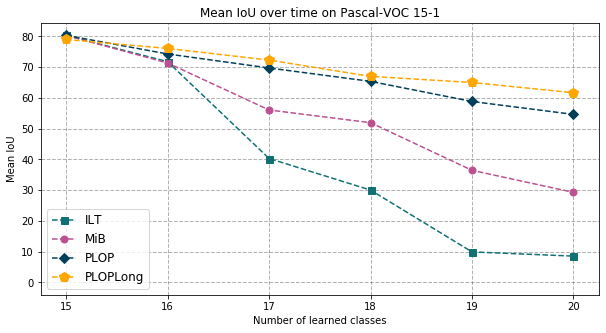
\includegraphics[width=0.7\linewidth]{images/seg/voc_15-1.png}
    \caption{\ac{mIoU} evolution on Pascal-VOC 2012 15-1. While MiB's \ac{mIoU} quickly
        deteriorates, PLOP and PLOPLong's \ac{mIoU} remains high, due to improved resilience to
        catastrophic forgetting.}
    \label{fig:seg_plot_voc_15-1}
\end{figure}

\begin{table*}[t]
    \centering
    \begin{adjustbox}{max width=\textwidth}
        \begin{tabular}{@{}l|cccc||cccc||cccc@{}}
            \toprule
                                                                       & \multicolumn{4}{c}{\textbf{100-50} (2 tasks)} & \multicolumn{4}{c}{\textbf{50-50} (3 tasks)} & \multicolumn{4}{c}{\textbf{100-10} (6 tasks)}                                                                                                                                                                         \\
            \textbf{Method}                                            & 0-100                                         & 101-150                                      & \textit{final}                                & \textit{avg}   & 0-50              & 51-150         & \textit{final}    & \textit{avg}   & 0-100             & 101-150           & \textit{final}    & \textit{avg}   \\
            \midrule
            ILT \scriptsize{\citep{michieli2019ilt}}                   & 18.29                                         & 14.40                                        & 17.00                                         & 29.42          & \tableindent 3.53 & 12.85          & \tableindent 9.70 & 30.12          & \tableindent 0.11 & \tableindent 3.06 & \tableindent 1.09 & 12.56          \\
            MiB \scriptsize{\citep{cermelli2020modelingthebackground}} & 40.52                                         & \textbf{17.17}                               & \textbf{32.79}                                & \textbf{37.31} & 45.57             & \textbf{21.01} & 29.31             & 38.98          & 38.21             & 11.12             & 29.24             & 35.12          \\
            PLOP                                                       & \textbf{41.87}                                & 14.89                                        & \textbf{32.94}                                & \textbf{37.39} & \textbf{48.83}    & \textbf{20.99} & \textbf{30.40}    & \textbf{39.42} & \textbf{40.48}    & \textbf{13.61}    & \textbf{31.59}    & \textbf{36.64} \\
            \bottomrule
        \end{tabular}
    \end{adjustbox}
    \caption{\textbf{ADE20k quantitative experiments} in \ac{mIoU} (\%).}
    \label{tab:seg_ade_sota}
\end{table*}

\begin{table}[t]
    \centering
    \begin{tabular}{@{}l|cccc@{}}
        \toprule
                                                      & \multicolumn{4}{c}{\textbf{VOC 10-1} (11 tasks)}                                                          \\
        \textbf{Method}                               & 0-10                                             & 11-20             & \textit{all}      & \textit{avg}   \\
        \midrule
        ILT \citep{michieli2019ilt}                   & \tableindent 7.15                                & \tableindent 3.67 & \tableindent 5.50 & 25.71          \\
        MiB \citep{cermelli2020modelingthebackground} & 12.25                                            & 13.09             & 12.65             & 42.67          \\
        PLOP                                          & 44.03                                            & 15.51             & 30.45             & 52.32          \\
        PLOPLong                                      & \textbf{61.06}                                   & \textbf{18.56}    & \textbf{40.83}    & \textbf{58.62} \\
        %{\color{red}\ourslong + OR} & \textbf{59.82} & \textbf{22.28} & \textbf{41.95} & \textbf{58.74}\\
        \bottomrule
    \end{tabular}
    \caption{\ac{mIoU} on Pascal-VOC 2012 10-1.}
    \label{tab:seg_voc_hard}
\end{table}

\begin{table}[t]
    \centering
    \begin{tabular}{@{}l|cccc@{}}
        \toprule
                                                      & \multicolumn{4}{c}{\textbf{ADE 100-5} (11 tasks)}                                                                      \\
        \textbf{Method}                               & 0-100                                             & 101-150                    & \textit{all}      & \textit{avg}      \\
        \midrule
        ILT \citep{michieli2019ilt}                   & \tableindent 0.08                                 & \tableindent 1.31          & \tableindent 0.49 & \tableindent 7.83 \\
        MiB \citep{cermelli2020modelingthebackground} & 36.01                                             & \tableindent 5.66          & 25.96             & 32.69             \\
        PLOP                                          & \textbf{39.11}                                    & \tableindent \textbf{7.81} & \textbf{28.75}    & \textbf{35.25}    \\
        % \ourslong & 24.78 & 10.23 & 19.97 & 30.03\\
        \bottomrule
    \end{tabular}
    \caption{\ac{mIoU} on ADE20k 100-5.}
    \label{tab:seg_ade_hard}
\end{table}



\paragraph{Pascal VOC 2012:} \autoref{tab:seg_voc_sota1} shows quantitative experiments on
VOC 19-1, 15-5, and 15-1. Both the proposed PLOP and PLOPLong outperform state-of-the-art
approaches, MiB \citep{cermelli2020modelingthebackground}, SDR \citep{michieli2021sdr}, and GIFS
\citep{cermelli2020fewshotcontinualsegm} on all evaluated settings by a significant margin. For
instance, on 19-1, the forgetting of old classes (1-19) is reduced by 4.39 percentage points (\pp)
while performance on new classes is greatly improved (+13.76 \pp), as compared to the best
performing method so far, MIB \citep{cermelli2020modelingthebackground}. On 15-5, our model is on par
with our re-implementation of MiB, and surpasses the original paper scores
\citep{cermelli2020modelingthebackground} by 1 \pp. On the most challenging 15-1 setting, general
continual models (EWC and LwF-MC) and ILT all have very low \ac{mIoU}. While MiB shows significant
improvements, PLOP still outperforms it by a wide margin. Furthermore, PLOP also significantly
outperforms the best performing approach on this setting, GIFS
\cite{cermelli2020fewshotcontinualsegm} (+6.11 \pp). Moreover, \ac{mIoU} for the joint model is
$77.40\%$, thus PLOP narrows the gap between \ac{CSS} and joint learning on every \ac{CSS} scenario. The
average \ac{mIoU} is also improved (+5.78 \pp) compared to GIFS, indicating that each \ac{CSS} step
benefits from the improvements related to our method. This is echoed by
\autoref{fig:seg_plot_voc_15-1}, which shows that while \ac{mIoU} for both ILT and MiB deteriorates
after only a handful of steps, PLOP's \ac{mIoU} remains very high throughout, indicating improved
resilience to catastrophic forgetting and background shift. Last but not least, while PLOP performs
better than PLOPLong on short setups (\eg 19-1, 15-5), PLOPLong performs better, however, on longer
\ac{CSS} benchmarks such as 15-1 (+2.81 \pp).



\paragraph{Cityscapes:} We also validate our method on Cityscapes in
\autoref{tab:seg_cityscapes_class}. In order to design a setting similar to Pascal-VOC 15-1 (6
tasks), we design the 14-1 setting. Also, we simulate a background class by folding together the
unlabeled classes. Here again, PLOP performs slightly better than MIB (+2.48 \pp on the old classes,
+0.16 \pp on the new ones, +1.15 \pp on average). Moreover, PLOPLong performs significantly better
(+3.59 \pp on the old classes, +2.13 \pp on the new ones, +3.15 \pp on average), indicating better
robustness to both catastrophic forgetting and background shift, especially when considering long
continual learning setups. To more precisely assess this phenomenon, we investigate the performance
of both methods when dealing with longer task learning sequences.

\paragraph{ADE20K:} \autoref{tab:seg_ade_sota} shows experiments on ADE 100-50, 100-10, and
50-50. This dataset is notoriously hard, as the joint model baseline \ac{mIoU} is only 38.90\%. ILT
has poor performance in all three scenarios. PLOP shows comparable performance with MiB on the short
setting 100-50 (only 2 tasks), improves by 1.09 \pp on the medium setting 50-50 (3 tasks),
and significantly outperforms MiB with a wider margin of 2.35 \pp on the long setting
100-10 (6 tasks). In addition to being better on all settings, PLOP showcased an increased
performance gain on longer \ac{CSS} (\eg 100-10) scenarios, due to increased robustness to catastrophic
forgetting and background shift.


\paragraph{Longer Continual Trainings:}We argue that \ac{CSS} experiments should push towards
more steps
\citep{wortsman2020supermasks,lomonaco2020ar1,douillard2020podnet,castro2018end_to_end_inc_learn} to
quantify the robustness of approaches w.r.t. catastrophic forgetting and background shift. We
introduce two novel and much more challenging settings with 11 tasks, almost twice as many as the
previous longest setting. We report results for VOC 10-1 in \autoref{tab:seg_voc_hard} (10 classes
followed by 10 times 1 class) and ADE 100-5 in \autoref{tab:seg_ade_hard} (100 classes followed by
10 times 5 classes). The second previous State-of-the-Art method, ILT, has a very low \ac{mIoU}
($<6$ on VOC 10-1 and practically null on ADE 100-5). Furthermore, the gap between PLOP and MiB is
even wider compared with previous benchmarks (\eg $\times$3.6 \ac{mIoU} on VOC for \ac{mIoU} of
base classes 1-10), which confirms the superiority of PLOP when dealing with the long continual
processes. Moreover, in such a case, PLOPlong really shines, bringing significant improvements
(+17.03 \pp on the old classes, +3.05 \pp on the new classes, +10.42 \pp on average) due to
a combination of cosine normalization (both on the classifier and Local POD) and its frozen
BatchReNormalization.

\subsubsection{Models Introspection}

We compare several distillation and classification losses on VOC 15-1 to stress the importance of
the components of PLOP and report results in \autoref{tab:seg_ablation_distill_classif}. All
comparisons are evaluated on a validation set made with 20\% of the training set, therefore results are
slightly different from the main experiments.

\paragraph{Distillation comparisons:} \autoref{tab:seg_ablation_distillation} compares different
distillation losses when combined with our pseudo-labeling loss. ILT \citep{michieli2019ilt} used
the naive knowledge distillation of \cite{hinton2015knowledge_distillation}. CSC \citep{park2020csc}
constrained spatial and channel correlation of intermediary features. This work bears similarity
with POD and Local POD, but it's much more computationally intensive as it computes pixel-by-pixel
correlation and not as performant. Finally, UNKD introduced in
\cite{cermelli2020modelingthebackground} performs better than the Knowledge Distillation (KD) of
\cite{hinton2015knowledge_distillation}, but not at every step (as indicated by the \textit{avg.}
value), which indicates instability during the training process. POD, proposed in
\cite{douillard2020podnet} (\autoref{chapter:regularization}), improves the results on the old
classes, but not on the new classes (16-20). In fact, due to too much plasticity, POD model likely
overfits and predicts nothing but the new classes, hence a lower \ac{mIoU}.  Finally, Local POD
leads to superior performance (+20 \pp) \wrt all metrics, due to its integration of both long and
short-range dependencies. This final row represents our full PLOP strategy.

\begin{table}
    \centering
    \caption{Comparison studies on Pascal-VOC 2012 15-1 on a validation subset of 20\% of the training set.}
    %\vspace*{-0.3cm}
    \label{tab:ablation_distill_classif}
    \begin{subtable}{0.5\textwidth}
        \centering
        \caption{Pseudo loss (\autoref{eq:pseudo_loss}) with different distillation losses.}
        %\vspace*{-0.2cm}
        \label{tab:ablation_distillation}
        \begin{tabular}{@{}l|cccc@{}}
            \toprule
            Distillation loss                       & 0-15           & 16-20             & \textit{all}   & \textit{avg}   \\
            \midrule
            %ILT \cite{michieli2019ilt}'s distill & 19.91 & \tableindent 5.49 & 16.48 & 49.43\\
            %CSC \cite{park2020csc} & 25.49 & \tableindent 4.72 & 20.48 & 44.97\\
            Knowledge Distillation                  & 29.72          & \tableindent 4.42 & 23.69          & 49.18          \\
            UNKD                                    & 34.85          & \tableindent 5.26 & 27.80          & 46.39          \\
            POD                                     & 43.94          & \tableindent 4.82 & 34.62          & 53.35          \\
            Local POD (\autoref{eq:local_pod_loss}) & \textbf{63.06} & \textbf{17.92}    & \textbf{52.31} & \textbf{65.71} \\
            \bottomrule
        \end{tabular}
    \end{subtable}
    \hfill
    \vspace{0.5cm}
    \begin{subtable}{0.5\textwidth}
        \centering
        \caption{Local POD loss (\autoref{eq:local_pod_loss}) with different classification losses.}
        %\vspace*{-0.2cm}
        \label{tab:ablation_classif}
        \begin{tabular}{@{}l|cccc@{}}
            \toprule
            Classification loss               & 0-15           & 16-20             & \textit{all}   & \textit{avg}   \\
            \midrule
            CE only on new                    & 12.95          & \tableindent 2.54 & 10.47          & 47.02          \\
            CE                                & 33.80          & \tableindent 4.67 & 26.87          & 50.79          \\
            UNCE                              & 48.46          & \tableindent 4.82 & 38.62          & 53.19          \\
            Pseudo (\autoref{eq:pseudo_loss}) & \textbf{63.06} & \textbf{17.92}    & \textbf{52.31} & \textbf{65.71} \\
            \midrule
            \textit{\small{Pseudo-Oracle}}    & \textit{63.69} & \textit{23.35}    & \textit{54.09} & \textit{66.05} \\
            %\textit{\small{Pseudo + corrected}} & \textit{66.88} & \textit{16.88} & \textit{54.98} & \textit{66.50}\\
            %\textit{\small{CE + all labels}}  & \textit{71.45} & \textit{10.78} & \textit{57.00} & \textit{67.04}\\
            \bottomrule
        \end{tabular}
    \end{subtable}
\end{table}






\paragraph{Classification comparisons:} \autoref{tab:seg_ablation_classif} compares different
classification losses when combined with our Local POD distillation loss. Cross-Entropy (CE)
variants perform poorly, especially on new classes. UNCE, introduced in
\citep{cermelli2020modelingthebackground}, improves by merging the background with old classes,
however, it still struggles to correctly model the new classes, whereas our pseudo-labeling
propagates more finely information of the old classes, while learning to predict the new ones,
dramatically enhancing the performance in both cases. This penultimate row represents our full PLOP
strategy. Also, notice that the performance for pseudo-labeling is very close to
\textit{(Oracle) Pseudo-good} (where the incorrect pseudo-labels are removed), which may constitute a
performance ceiling of our uncertainty measure. A comparison between these two results illustrates
the relevance of our entropy-based uncertainty estimate. \textit{(Oracle) Pseudo-corrected} is
similar to the previous oracle but instead fix the incorrect pseudo-labels; note that not all labels
are present as some pixels were not even pseudo-labelized due to their high uncertainty. Finally,
\textit{(Oracle) CE + all labels} has access to all labels of previous and current classes
$\mcC^{1:t}$.

\subsubsection{Robustness to class ordering}

Continual learning methods may be prone to instability. It has already been shown in related
contexts \citep{kim2019medic} that class ordering can have a large impact on performance.
Unfortunately, in real-world settings, the optimal class order can never be known beforehand: thus,
the performance of an ideal \ac{CSS} method should be as invariant to class order as possible. In all
experiments done so far, this class order has been kept constant, as defined
by \cite{cermelli2020modelingthebackground}. We report results in \autoref{fig:seg_order_voc_15-1}
as boxplots obtained by applying 20 random permutations of the class order on VOC 15-1. We report in
\autoref{fig:seg_order_voc_15-1} (from left to right) the \ac{mIoU} for the old, new classes, all
classes, and average over \ac{CSS} steps. In all cases, PLOP surpasses MiB in terms of avg \ac{mIoU}.
Furthermore, the standard deviation (\eg 10\% \vs 5\% on \textit{all}) is always significantly
lower, showing the excellent stability of PLOP compared with existing approaches. Moreover,
PLOPLong, while having more variance on the new classes, performs better overall as compared to
PLOP, not to mention MiB. This is due to the fact that PLOPLong, due to improved distillation loss
(at prediction and Local POD levels) and batch re-normalization that allows to better retain
information of the old classes, which again is more conspicuous on longer \ac{CSS} scenarios.


\begin{figure}
    \centering
    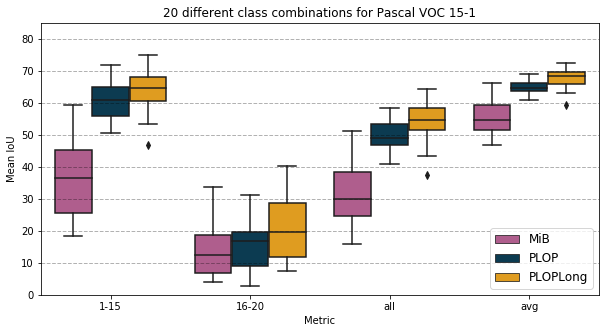
\includegraphics[width=0.7\linewidth]{images/seg/order_voc_15-1.png}
    \vspace*{-0.3cm}
    \caption{\textbf{Robustness to class ordering:} Boxplots of the \ac{mIoU} of initial classes (1-15), new (16-20), all, and average for
        20 random class orderings. PLOP is significantly better and more stable than MiB. PLOPLong
        further improves upon PLOP by better retaining old class information.}
    \label{fig:seg_order_voc_15-1}
\end{figure}


\subsection{Object Rehearsal experiments}

\subsubsection{Quantitative Evaluations}

\begin{table*}[t]
    \centering
    \caption{Comparison of rehearsal-based methods on Pascal-VOC 2012 15-1 overlap in Mean IoU (\%). We only consider the time overhead spent after the first task whose computation overhead is similar for all methods.}
    \vspace*{-0.3cm}
    \label{tab:voc_rehearsal_learning}
    \begin{tabular}{@{}l|ccc|cccc@{}}
        \toprule
                                                                & \multicolumn{7}{c}{\textbf{15-1} (6 tasks)}                                                                                                                                              \\
        \textbf{Method}                                         & \textbf{Rehearsal}                          & \textbf{Memory} (Mb) $\downarrow$ & \textbf{Time} (Hours) $\downarrow$ & 0-15           & 16-20          & \textit{all}   & \textit{avg}   \\
        \midrule
        PLOP                                                    & ---                                         & 0                                 & 1.8                                & 65.12          & 21.11          & 54.64          & 67.21          \\
        PLOPLong                                                & ---                                         & 0                                 & 1.8                                & 72.00          & 26.66          & 61.20          & 70.02          \\
        %HRHF \cite{huang2021halfrealhalffake} & DeepInversion & 0 & 5.9 & 72.40 & 39.60 & 64.60 & \\
        \hdashline
        Yu et al.\cite{yu2020continualsegmentationselftraining} & Unlabeled COCO                              & 20,000                            & 7.0                                & 71.40          & 40.00          & 63.60          &                \\
        PLOP                                                    & Unlabeled COCO                              & 20,000                            & 1.4                                & 72.57          & 45.08          & 66.03          & 71.85          \\
        PLOP                                                    & Unlabeled VOC                               & 2,000                             & 1.4                                & 75.32          & 52.59          & 69.91          & 75.21          \\
        %PLOP & Partial VOC & 2,000 & \tbd & 74.91 & 54.55 & 70.06 & 75.41 \\
        %PLOPv2 & Partial VOC & 2,000  & \tbd & 76.87 & 56.07 & 71.92 & 74.88\\
        \hdashline
        PLOPLong                                                & Partial VOC                                 & 2.2                               & 2.6                                & 74.14          & 38.87          & 65.74          & 72.02          \\
        PLOPLong                                                & Partial VOC                                 & 22                                & 2.6                                & \textbf{74.18} & 43.22          & 66.81          & \textbf{72.48} \\
        PLOPLong                                                & Object VOC                                  & 0.26                              & 2.7                                & 73.32          & 42.86          & 66.07          & 72.21          \\
        PLOPLong                                                & Object VOC                                  & 2.6                               & 2.7                                & 73.79          & \textbf{45.78} & \textbf{67.12} & \textbf{72.42} \\
        \midrule
        Joint model                                             & ---                                         & ---                               & ---                                & 79.10          & 72.60          & 77.40          & ---            \\
        \bottomrule
    \end{tabular}
\end{table*}


\paragraph{Pascal-VOC 15-1:} We now allow \ac{CSS} models to store information from the previous
steps and classes: in such a case, the overall model efficiency can be understood as to what extent
it allows to find a good trade-off between its accuracy (as measured by the aforementioned standard
metrics) and the memory footprint of the stored images or objects. Methods such as HRHF
\citep{huang2021halfrealhalffake} can not easily be understood in these terms as they do not store
data, strictly speaking, but rather use deep inversion \citep{yin20deepinversion} techniques to
generate synthetic data, which comes at a high time requirement: thus, we exclude this method from
our comparisons. We first consider the challenging Pascal-VOC 15-1 setting in
\autoref{tab:seg_voc_rehearsal_learning}. We use PLOP and PLOPLong as baselines with 0 memory
overhead, as both models only use data from the current task. Moreover, we compare with
\cite{yu2020continualsegmentationselftraining}, where an unlabeled external dataset such as COCO
\citep{lin2014mscocodataset} is used through pseudo-labeling to improve performance on Pascal-VOC,
as both datasets present significant overlap in terms of classes and domains. We reimplemented their
method and also considered PLOP in this configuration. Using the external COCO provide PLOP an
important gain of \ac{mIoU} for both old classes (+7 \pp) and new classes (+24
\pp). Furthermore, PLOP with COCO is significantly more performant than \cite{yu2020continualsegmentationselftraining}'s model
(+5.43 \pp) despite the latter was designed explicitly to use such unlabeled external
dataset. Notice also how PLOPLong, without any kind of rehearsal, remains equivalent to
\cite{yu2020continualsegmentationselftraining} in terms of \ac{mIoU} on 0-15 (72.00\% \vs 71.40\%),
despite the latter using a large pool of data (+20Go). Perhaps counter-intuitively the gain is
located on the new classes (26.66\% \vs 40.00\%) as the rehearsal effect has a regularizing effect
leading to less over-predicting of the recent classes. A drawback of using COCO is that the visual
domain is not exactly the same as VOC, therefore we also considered using PLOP with a rehearsal of
the unlabeled VOC. Without surprise, it results in a much better overall performance (+3.88
\pp compared to using COCO). Another setup that we consider is the image rehearsal
paradigm, where, at each step, we keep a number of (randomly selected) images along with their
segmentation map. These segmentation maps are, however, incomplete, due to the nature of the \ac{CSS}
problem (see \autoref{sec:seg_object_rehearsal}): hence, we refer to this setting as partial VOC. We
consider two amounts of images to keep: 10 images per class (22 Mb) and 1 image per class (2.2 Mb).
PLOPLong largely benefits from this rehearsal, most notably on new classes (16-20); with a gain up to
16.56 \pp. Finally, we compare our novel Object Rehearsal denoted by ``\textit{object
    VOC}'' where we store either one object per class (0.26 Mb) or 10 objects per class (2.6 Mb). As
shown on \autoref{tab:seg_voc_rehearsal_learning}, The proposed object rehearsal, in addition to
being significantly more memory efficient than whole image rehearsal (8.5$\times$ less space used),
is equivalent or better in terms of \ac{mIoU}; especially for new classes (2.56 \pp). The
ensemble of our experiments proves that rehearsal, when the partial or missing labeling is carefully
handled, can provide important performance gain. Furthermore, our novel object rehearsal manages to
strike the best trade-off with a minimal memory overhead without impacting its performance.

\begin{comment}
\begin{figure}
    \centering
    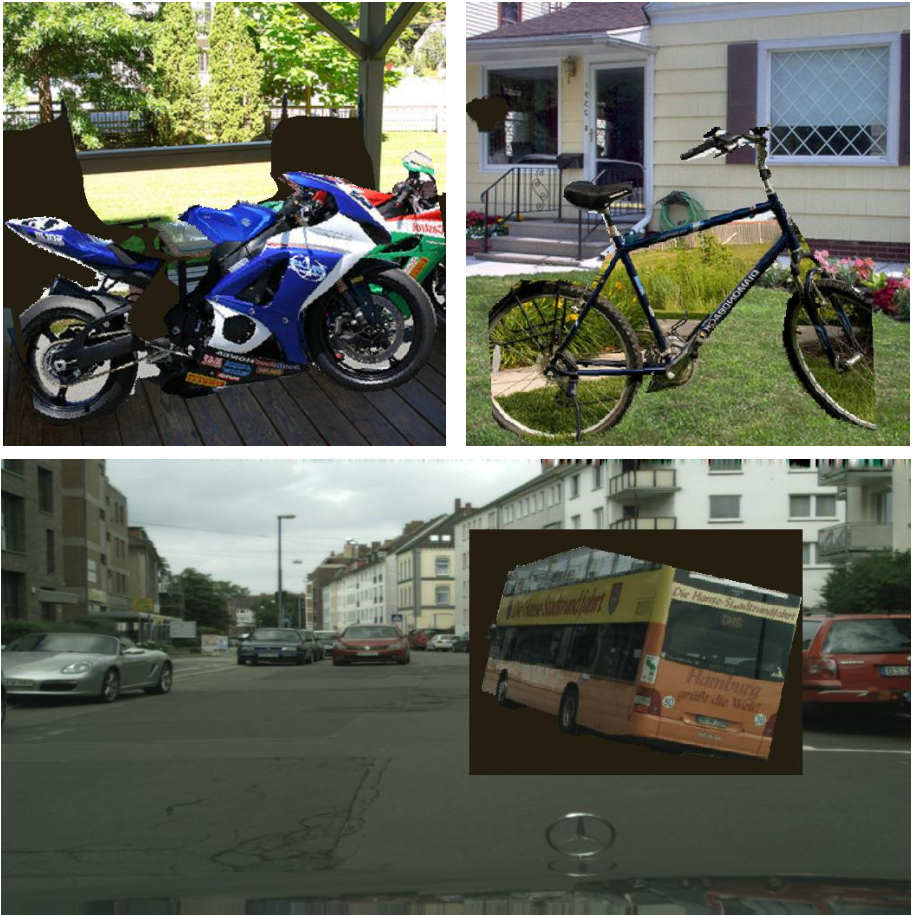
\includegraphics[width=0.5\linewidth]{images/seg/object_pasting.pdf}
    \caption{Pasted object for rehearsal in three images. Top row shows the pasting of a
        \texttt{motorbike} and a \texttt{bicycle} in Pascal-VOC, and bottom row shows the pasting of
        a \texttt{bus} in Cityscapes.}
    \label{fig:seg_object_pasting}
\end{figure}
\end{comment}

\paragraph{Cityscapes:} We propose more experiments with Object Rehearsal in
\autoref{tab:seg_cityscapes_rehearsal} where we apply our model on Cityscapes 14-1. For the rehearsal,
we sample either 10 images or objects per class. Cityscapes images are particularly large (even
resized to $512 \times 1024$)  and "empty" (most of it is road and sky). Consequently, the memory
overhead is extremely important compared object rehearsal (117 \vs 0.8). We show that both our novel
image and object rehearsal improve performance of the already competitive PLOPLong, and with object
rehearsal providing the large gain (+9 \pp in \textit{all}).

t\begin{table}[t]
    \centering
    \begin{adjustbox}{max width=\textwidth}
        \begin{tabular}{@{}l|cc|cccc@{}}
            \toprule
                                                                       & \multicolumn{6}{c}{\textbf{14-1} (6 tasks)}                                                                                       \\
            \textbf{Method}                                            & \textbf{Rehearsal}                          & \textbf{Memory} & 1-14           & 15-19          & \textit{final} & \textit{avg}   \\
            \midrule
            MiB \scriptsize{\citep{cermelli2020modelingthebackground}} & ---                                         & 0               & 55.11          & 12.91          & 44.56          & 49.76          \\
            PLOP                                                       & ---                                         & 0               & 56.59          & 13.07          & 45.71          & 51.28          \\
            PLOPLong                                                   & ---                                         & 0               & 58.60          & 15.04          & 47.71          & 54.31          \\
            PLOPLong                                                   & Partial                                     & 117.0           & \textbf{58.93} & 19.55          & 49.09          & \textbf{55.74} \\
            PLOPLong                                                   & Object                                      & 0.8             & 57.82          & \textbf{23.13} & \textbf{49.15} & 54.80          \\
            \bottomrule
        \end{tabular}
    \end{adjustbox}
    \caption{\textbf{Cityscapes quantitative experiments with rehearsal} on Cityscapes 14-1 overlap in \ac{mIoU} (\%).}
    \label{tab:seg_cityscapes_rehearsal}
\end{table}

\begin{table}[t]
    \centering
    \begin{tabular}{@{}llc|c|cc|r@{}}
        \toprule
                                &                 &                &                                & \multicolumn{2}{c}{\textbf{15-1} (6 tasks)}                         \\
        \textbf{Type}           & \textbf{Mixing} & \textbf{Erase} & \textbf{Memory} $\downarrow$   & \textit{final}                              & \textit{avg}   &      \\
        \midrule
        \multirow{2}{*}{Image}  & Mixup           & ---            & \multirow{2}{*}{22.20}         & 61.77                                       & 69.88          & I    \\
                                & \,\,\,\,\,---   & ---            &                                & 66.81                                       & \textbf{72.48} & II   \\
        \hline
        \multirow{3}{*}{Patch}  & Pasting         & All            & \multirow{3}{*}{4.50}          & 55.45                                       & 66.35          & III  \\
                                & Pasting         & ---            &                                & 63.41                                       & 70.75          & IV   \\
                                & Pasting         & Foreground     &                                & 66.28                                       & 71.66          & V    \\
        \hline
        \multirow{5}{*}{Object} & Mixup           & ---            & \multirow{5}{*}{\textbf{2.60}} & 63.25                                       & 70.91          & VI   \\
                                & Mixup           & Foreground     &                                & 64.45                                       & 71.65          & VII  \\
                                & Pasting         & All            &                                & 52.26                                       & 65.97          & VIII \\
                                & Pasting         & ---            &                                & 63.12                                       & 70.52          & IX   \\
                                & Pasting         & Foreground     &                                & \textbf{67.12}                              & \textbf{72.42} & X    \\
        \bottomrule
    \end{tabular}
    \caption{\textbf{Rehearsal alternatives} on Pascal-VOC 2012 in \ac{mIoU} (\%). Object/Patch-based methods
        with 10 objects/patches per class, and Image-based with 10 images per class. All
        experiments done with PLOPLong.}
    \label{tab:seg_rehearsal_alternative}
\end{table}


\begin{figure}
    \centering
    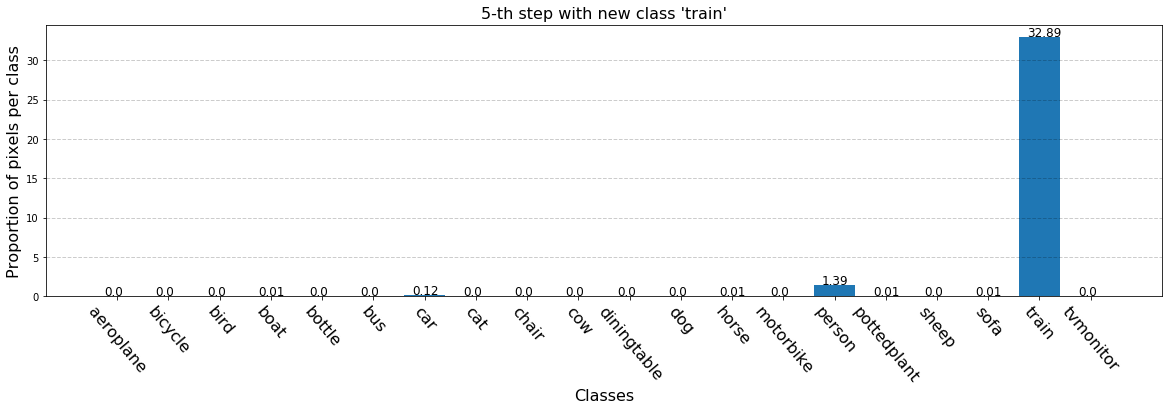
\includegraphics[width=\linewidth]{images/seg/distribution_5step_voc.png}
    \vspace*{-0.3cm}
    \caption{\textbf{Pixel distribution per class} during the $5^{\text{th}}$ step of Pascal-VOC
        15-1.}
    \label{fig:seg_distribution_voc_5th}
\end{figure}

\begin{figure*}
    \centering
    \includegraphics[width=\linewidth]{images/seg/visualization2.pdf}
    \caption{\textbf{Visualization of the predictions} of MiB, PLOP, PLOPLong, and PLOPLong with Object
        Rehearsal on three test images at the $6^\text{th}$ and final step on VOC 15-1 scenario. The
        first image contains \texttt{car}, \texttt{cow}, and \texttt{person}; the second
        \texttt{plane} and \texttt{bus}, and the third \texttt{bicycle} and \texttt{person}. While
        MiB does not manage to predict the correct classes, and tends to overpredict the most recent
        ones (\eg \texttt{train} in light green). PLOP mostly grasp the correct classes, though
        sometimes with imprecision. PLOPLong and \textit{a fortiori} PLOPLong + Object rehearsal
        captures all existing classes, with the latter predicting almost perfect segmentation masks,
        compared to the ground-truth.}
    \label{fig:seg_visualization}
\end{figure*}

\subsubsection{Object Rehearsal Introspection}

\autoref{tab:seg_rehearsal_alternative} draws a comparison between several rehearsal alternatives in
\ac{CSS}. We split methods according to three criterions: ``\textit{type}'' denotes whether we store a
whole image, an object, or a patch. For both object and patch, we only rehearse a small amount of the
images: in object, only the pixel's objects are used while for a patch, we use the pixel's object and
the close surrounding pixels that contain background information. We insert the rehearsal data
according to ``\textit{mixing}'', either by pasting (see \autoref{sec:seg_object_rehearsal}), by
mixing pixels according to mixup \citep{hingyi2018mixup} rule, or in the case of image rehearsal, no
mixing is done. Finally, we consider two erasing methods: either all pixels are erased
(\textit{All}), or only pixels belonging to non-background classes are erased (\textit{Foreground}).
Note that for the latter method, it includes classes detected via pseudo-labeling. For all methods,
we randomly select 10 images/patches/objects per class for rehearsal. Without surprise, Patch
(III-V) and Object-based (VI-X) rehearsal are more data-efficient than images (I and II) (4.50 and
2.60 \vs 22.20 Mb). Mixing the rehearsed data with mixup (VI and VII) is less efficient than direct
pasting (III, IV, and VIII-X) because segmentation, contrary to classification, requires sharp
boundaries \citep{chen2020semeda}. We considered rehearsing each patch/object without mixing, but
because their shape may vary, no batching is possible resulting in a slower training. Therefore, we
investigate mixing patches/objects while erasing all others pixels (III and VIII). This does not
work, which is probably linked to the altered statistics of the batch normalization. On the other
hand, we found that a selective erasing that remove foreground objects (V, VII, and X) while keeping
the background of the destination image proved to be very effective (63.12\% to 67.12\% \textit{all}
\ac{mIoU} for object). This confirmed our intuition that pasting in segmentation is a delicate
operation that may lead to confusion in the network, particularly on object boundaries. The erased
pixels are replaced by gray pixels. We considered more complicated approaches such as in-painting
\citep{fang2019instaboost} or textures filling \citep{mallikarjuna2006kth-tips}, but were slightly
less effective than our simpler solution. Overall, through careful design, we manage to get the best
performance using our novel object rehearsal which was also the most memory-efficient.

\begin{figure}
    \centering
    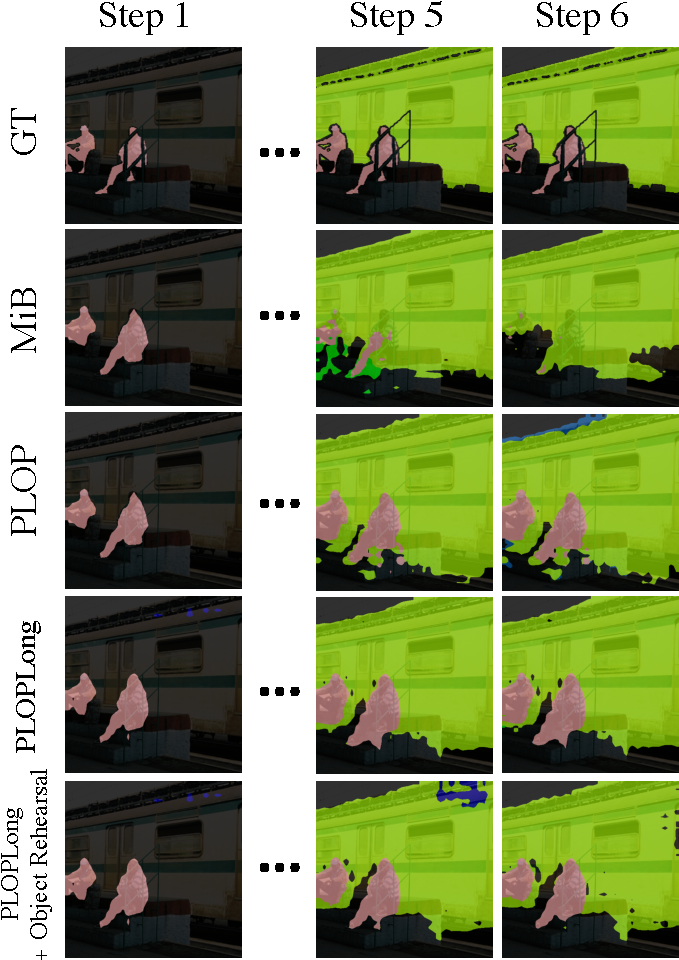
\includegraphics[width=0.7\linewidth]{images/seg/visualization_gt_shift2.pdf}
    \caption{\textbf{Visualization of the predictions with a background shift} of MiB, PLOP, PLOPLong, and PLOPLong with Object
        Rehearsal across time in VOC 15-1 on a test set image. At steps 1-4 only class
        \texttt{person} has been seen. At step 5, the class \texttt{train} is introduced, causing
        dramatic background shift. While MiB overfits on the new class and forget the old class,
        PLOP is able to predict both classes correctly. PLOPLong and PLOPLong + Object Rehearsal
        further refine the predicted masks, resulting in much sharper boundaries.}
    \label{fig:seg_visualization_gt_shift}
\end{figure}

\paragraph{Rehearsal alleviates pseudo-labeling's limitation:} All previous methods, PLOP
and PLOPLong included, did not consider rehearsal-learning. While popular in image classification, it
has not been explored for continual segmentation. An attentive reader may wonder if rehearsal
learning can provide benefits given the fact that our pseudo-labeling can uncover ``hidden'' old classes
in the images. Even a perfect pseudo-labeling (considered in \autoref{tab:seg_ablation_classif}) may
fail in some particular data situation where the class distribution of a step is almost Dirac. We
show in \autoref{fig:seg_distribution_voc_5th} the distribution of pixels per class at the
$5^{\text{th}}$ step of Pascal-VOC 15-1. The new class to learn, \texttt{train}, is abundant but
also almost alone but the class \texttt{person}. In this case, no amount of pseudo-labeling can
uncover previous classes like \texttt{bicycle} or \texttt{cat}. Our proposed rehearsal learning is
complementary to our pseudo-labeling loss where the former can reduce the weakness for the latter in
some cases.

\subsection{Visualization}

\autoref{fig:seg_visualization} shows the predictions at the $6^\text{th}$ and final step of VOC
15-1 for four different models: MiB, PLOP, PLOPLong, and PLOPLong with Object Rehearsal. MiB
struggles to even find the correct classes: in the first image the \texttt{car} is predicted as
\texttt{train}, in the second the \texttt{plane} as \texttt{train}, and in the third no classes are
detected. On the other hand, PLOP always manages to pick up the present classes, although sometimes
with imperfection. PLOPLong further refines results, and the addition of Object Rehearsal produces a
sharp and near perfect masks compared to the ground-truths (GTs). We showcased the harmful effect of
background shift in \autoref{fig:seg_visualization_gt_shift} where the class \texttt{person} is
learned at $1^\text{st}$ step and the class \texttt{train} at $5^\text{th}$ step. MiB completely
forgets the former class and overpredicts the latter. The background shift is efficiently mitigated
with pseudo-labeling showed in the third row of PLOP. Our efficient proposition of object
rehearsal allows further refinement of the predicted masks resulting in sharper boundaries.

\section{Conclusion}
\label{sec:seg_conclusion}

Continual Semantic Segmentation (\ac{CSS}) is an emerging but challenging computer vision domain. In this
paper, we highlighted two major issues in \ac{CSS}: catastrophic forgetting and background shift. To deal
with the former, we proposed Local POD, a multi-scale distillation scheme that preserves both long
and short-range spatial statistics between pixels. This leads to an effective balance between
rigidity and plasticity for \ac{CSS}, which in turns alleviates catastrophic forgetting. We then tackled
background shift with an efficient uncertainty-based pseudo-labeling loss. It completes the
partially-labeled segmentation maps, allowing the network to efficiently retain previously learned
knowledge. Afterwards, We showed that carefully designed structural changes to the model could
improve performance on long \ac{CSS} scenarios, namely a cosine normalization adaptation of the
classifier and Local POD followed by a modified batch normalization. Finally, we proposed to
introduce rehearsal learning to \ac{CSS}, one based on partially-labeled whole image rehearsal, and the
other --much more memory-efficient-- consisting in object rehearsal. The latter further refines our
already effective model performance and enables real world applications of \ac{CSS} with a stringent
memory constraint. We evaluated the proposed PLOPLong, with or without object rehearsal, on three
datasets and over twelve different benchmarks. In each, we showed that our model performs
significantly better than all existing baselines. Finally, we qualitatively validate our model
through extensive ablations in order to better understand the performance gain.

\cleardoublepage
\let\leftmark=\oldleftmark

\acresetall
\chapter{Dynamic Strategy with Transformers}
\label{chapter:dynamic}

\begin{chapabstract}
    Continual models aim to learn an ever-growing number of tasks. Dynamic architectures expand
    their parameters to tackle this increasing complexity. However,
    existing approaches often require a task identifier at test-time, need complex tuning to balance
    the growing number of parameters, and barely share any information across tasks. As a result,
    they struggle to scale to a large number of tasks without significant overhead.\\
    In this chapter, we propose a transformer architecture based on a dedicated encoder/decoder
    framework. Critically, the encoder and decoder are shared among all tasks. Through a dynamic
    expansion of special tokens, we specialize each forward of our decoder network on a task
    distribution. Our strategy scales to a large number of tasks while having negligible memory and
    time overheads due to strict control of the expansion of the parameters. Moreover, as a result,
    this efficient strategy doesn't need any hyperparameter tuning to control the network's
    expansion.\\
    We evaluate our model on multiple datasets and show the interest of our parameter expansion strategy,
    striking the right balance between performance and overhead. We also extensively ablate our
    model to highlight each component contribution.

    \begin{itemize}
        \item \fullcite{douillard2021dytox}
    \end{itemize}

\end{chapabstract}
\newpage

\minitoc
\chapterwithfigures{\nameref*{chapter:dynamic}} \chapterwithtables{\nameref*{chapter:dynamic}}

\ifthenelse{\boolean{skipDyna}}{\endinput}{}


\section{Introduction}
\label{sec:dytox_intro}


Recent works expand the network architectures or re-arrange their internal structures using dynamic
strategies (see \autoref{sec:related_structural}). Unfortunately at test-time, they require to know
the task to which the test sample belongs --- in order to know which parameters should be used. More
recently, DER \citep{yan2021der} and Simple-DER \citep{li2021preserve} discarded the need for this
task identifier by learning a single classifier on the concatenation of all produced embeddings by
different subsets of parameters. Yet, these strategies induce an important memory overhead when
tackling a large number of tasks, and thus need complex pruning as post-processing.

To improve the ease of use of continual learning frameworks for real-world applications, we aim to
design a dynamically expandable representation (almost) ``for free'' by having the three following
properties:

\begin{enumerate}
    \item \textbf{limited memory overhead} as the number of tasks grows,
    \item \textbf{limited time overhead} at test time,
    \item \textbf{no setting-specific hyperparameters} for improved robustness when faced to an unknown
          (potentially large) number of tasks.
\end{enumerate}

%\#1 \textbf{limited memory overhead} as the number of tasks grows, \#2 \textbf{limited
%    time overhead} at test time and \#3 \textbf{no setting-specific hyperparameters} for improved
%robustness when faced to an unknown (potentially large) number of tasks.

To this end, we leverage the computer vision transformers (refer to \autoref{sec:related_cv}).
Transformers \citep{vaswani2017transformer} offer a very interesting framework to satisfy the
previously mentioned constraints. Indeed, we build upon this architecture to design a
\textbf{encoder/decoder strategy}: the encoder layers are shared among all members of our dynamic
network; the unique decoder layer is also shared, but its forward pass is specialized by a
\textbf{task-specific learned token} to produce task-specific embeddings. Thus, the memory growth of
the dynamic network is extremely limited: only a 384d vector per task, validating property \#1.
Moreover, this requires no hyperparameter tuning (property \#3). Finally, the decoder is explicitly
designed to be computationally lightweight (satisfying property \#2). We nicknamed our framework,
DyTox, for \textbf{DYnamic TOken eXpansion}.

Our strategy is robust to different settings, and can easily scale to a large number of tasks with
minimal time and memory overheads. In particular, we validate the efficiency of our approach on
CIFAR100, ImageNet100, and ImageNet1000 for multiple settings. We also perform ablations confirming
the soundness of our dynamic strategy. In this chapter, we focus on continual dynamic networks
(refer to \autoref{sec:related_structural}) that expand their parameters coupled with rehearsal
learning (\autoref{sec:related_rehearsal}). Moreover, to satisfy our desiderata listed previously,
we base our framework on the recent Transformer architecture (see \autoref{sec:related_cv}).

\paragraph{Positioning with respect to PODNet} Note that while our methods PODNet
(\autoref{sec:podnet}) and DyTox (presented in this chapter) are both designed for class-incremental
image classification, they differ in terms of both objective and benchmark: PODNet aims to constrain
the features drift to reduce forgetting, while DyTox conditions features to a particular task.
Moreover, PODNet, a metric-based model, requires a larger initial task size to perform well.
Therefore, PODNet was evaluated when half of the dataset's classes are seen in the first step. On
the other hand, DyTox is considered here in the setting of \citet{yan2021der} where all steps,
including the first one, bring an equal number of new classes.

\section{DyTox transformer model}
\label{sec:dytox_model}

\begin{figure*}
    \centering
    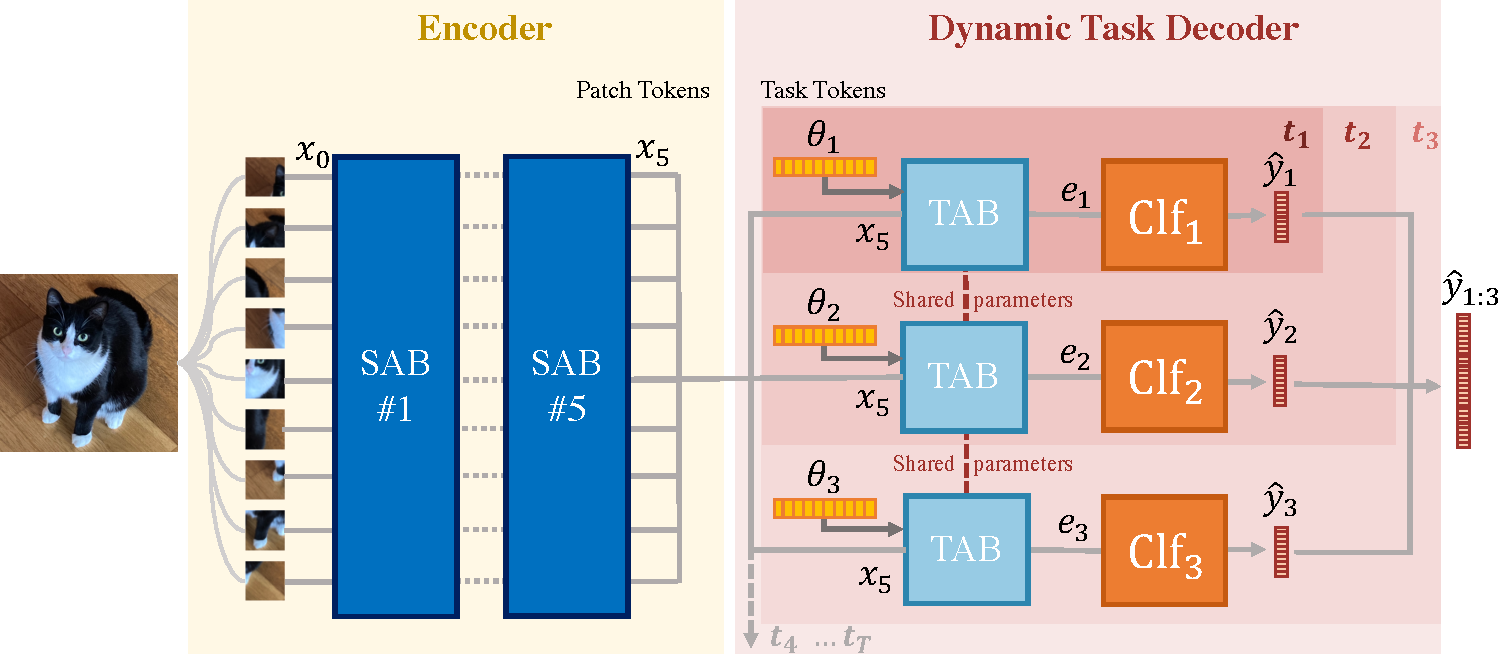
\includegraphics[width=0.95\textwidth]{images/dytox/dytox.pdf}
    \caption{\textbf{DyTox transformer model}. An image is first split into multiple patches,
    embedded with a linear projection. The resulting patch tokens are processed by 5 successive
    Self-Attention Blocks (SAB) (\autoref{sec:related_cv}). For each task ($t = 1\dots T$), the processed
    patch tokens are then given to the Task-Attention Block (TAB) (\autoref{sec:dytox_tab}): each forward
    through the TAB is modified by a different task-specialized token $\theta_t\, \text{for}\, t \in
        \{1 \dots T\}$ (\autoref{sec:dytox_ensembling_tab}). The $T$ final embeddings are finally given
    separately to independent classifiers $\text{Clf}_t$ each predicting their task's classes $C^t$.
    All $|C^{1:T}|$ logits are activated with a sigmoid. For example, at task $t=3$, one forward is
    done through the SABs and three task-specific forwards through the unique TAB.}
    \label{fig:dytox_model}
\end{figure*}

\label{sec:dytox_problem}

%Our goal is to learn a unified model that will classify an increasingly growing number of classes,
%introduced in a fixed amount of steps $T$. At a given step $t \in \{1 \dots T\}$, the model is
%exposed to new data belonging to new classes. Specifically, it learns from samples $\{(x_i^t,
%      y_i^t)\}_{i}$, where $x_i^t$ is the $i$-th image of this task $t$ and $y_i^t$ is the associated
%label within the label set $\mcC^t$. All task label sets are exclusive: $\mcC^0 \cap \mcC^1 \dots
%      \mcC^T = \emptyset$. The main challenge is that the data are fully available only temporarily:
%following most previous works, only a few samples from previous tasks $\{1 \dots t-1\}$ are
%available for training at step $t$ as rehearsing data. Yet, the model should remain able to classify
%test data coming from all seen classes $\mcC^{1:t}$. A table of notations is provided in the
%supplementary materials.

We evaluate our framework in the \acf{CIL} setting (\autoref{sec:related_continual}) where each task
brings an equal number of new classes. We also use rehearsal learning
(\autoref{sec:related_rehearsal}). The \autoref{fig:dytox_model} displays our DyTox framework, which
is made of several components (SAB, TAB, and Task Tokens) that we describe in the following
sections.

\subsection{Background}
\label{sec:dytox_vit}

The vision transformer \citep{dosovitskiy2020vit} has three main components: the patch tokenizer, the
encoder made of Self-Attention Blocks (SABs), and the classifier. We described in the related work
(\autoref{sec:related_cv}) the general architecture. A SAB is depicted in \autoref{fig:dytox_sab}.

\begin{figure}
    \centering
    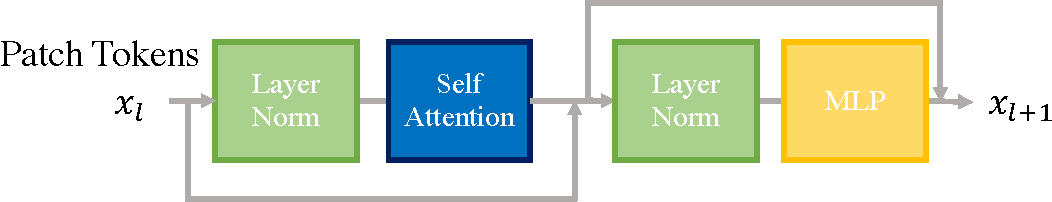
\includegraphics[width=1\textwidth]{images/dytox/sab.pdf}
    \caption{\textbf{The Self-Attention Block (SAB)} combines a Self-Attention (SA), two Layer
        Norms, and one MLP with a single hidden layer. As in a ResNet, two shortcuts are used with
        element-wise addition.}
    %\vspace{-2em}
    \label{fig:dytox_sab}
\end{figure}

Importantly, recall that in the original vision transformer ViT \citep{dosovitskiy2020vit}, a learned
vector called the ``\textit{class token}'' is appended to the patch tokens after the tokenizer. This
special class token, when processed after all the SABs, is given to a linear classifier with a
softmax activation to predict the final probabilities. However, more recent works, as CaiT
\citep{touvron2021cait}, propose instead to introduce the class token only at the ultimate or
penultimate SAB to improve classification performance.

\subsection{Task-Attention Block (TAB)}
\label{sec:dytox_tab}

Contrary to previous transformer architectures, we don't have a class token, but rather what we
nicknamed ``\textbf{task tokens}''; the learned token of the $i^{th}$ task is denoted $\theta_i$.
This special token will only be added at the last block. To exploit this task token, we define a new
attention layer, that we call the Task-Attention. It first concatenates the patch tokens $x_L$
produced by the ultimate SAB with a task token $\theta_i$:
%
\begin{equation}
    z_i = [\theta_i, x_L] \, \in \mathbb{R}^{(\mathbb{N} + 1) \times \mathbb{D}}\,.
    \label{eq:dytox_concat_cls_token}
\end{equation}
%
This is then given to the Task-Attention (TA), inspired by the Class-Attention of Touvron et al.
\citep{touvron2021cait}:
%
\begin{equation}
    \begin{aligned}
        Q_i & =W_{q} \theta_i\,,                                                      \\
        K_i & =W_{k} z_i\,,                                                           \\
        V_i & =W_{v} z_i\,,                                                           \\
        A_i & =\operatorname{Softmax}\left(Q_i \cdot K_i^{T} / \sqrt{d / h}\right)\,, \\
        O_i & = W_{o} A_i V_i+b_{o} \, \in \mathbb{R}^{1 \times \mathbb{D}}\,,
    \end{aligned}
    \label{eq:dytox_ca_layer}
\end{equation}
%
with $d$ being the embedding dimension, and $h$ the number of attention heads
\citep{vaswani2017transformer}. Contrary to the classical Self-Attention, the Task-Attention defines
its query ($Q_i$) only from the task-token $\theta_i$ without using the patch tokens $x_L$. The
Task-Attention Block (TAB) is then a variation of the SAB where the attention is a Task-Attention
(TA):
\begin{equation}
    \begin{aligned}
        c^{\prime}       & =c+\operatorname{TA}\left(\operatorname{Norm}_1\left(z\right)\right)\,,                    \\
        c^{\prime\prime} & =c^{\prime}+\operatorname{MLP}\left(\operatorname{Norm}_2\left(c^{\prime}\right)\right)\,.
    \end{aligned}
    \label{eq:dytox_ca_block}
\end{equation}
Overall, our new architecture can be summarized by the repetition of SA Blocks
$\{\operatorname{SAB}_l\}_{l=1}^{L}$ (defined in \autoref{eq:related_sa}) ended by a single TA Block
$\operatorname{TAB}$ (defined in \autoref{eq:dytox_ca_block}):
%
\begin{equation}
    e_i = \operatorname{TAB} \circ\, ([\theta_i,\, \operatorname{SAB}_{l=L} \circ\, ... \operatorname{SAB}_{l=1}(x_0)]) \in \mathbb{R}^D\,.
    \label{eq:dytox_cab_sab}
\end{equation}
%
The final embedding $e_i$ is fed to a classifier $\operatorname{clf}$ made of a
$\operatorname{Norm}_c$ and a linear projection parametrized by $\{W_c, b_c\}$:
%
\begin{equation}
    \tilde{y}_i = \operatorname{Clf}(e_i) = W_c \operatorname{Norm}_c(e_i) + b_c\,.
\end{equation}

\subsection{Dynamic task token expansion}
\label{sec:dytox_ensembling_tab}
We defined in the previous section our base network, made of a succession of SABs and ended by a
single TAB. As detailed, the TAB has two inputs: the patch tokens $x_L$ extracted from the image and
a learned task-token $\theta_i$. We'll now detail how our framework evolves in a continual situation
at each new step.

During the first step, there is only one task token $\theta_1$. At each new step, we propose to
expand our parameter space by creating a new task token while keeping the previous ones. Thus, after
$t$ steps, we have $t$ task tokens ($\theta_i\,\text{for}\, i\in \{1 \dots t\}$). Given an image $x$
--- belonging to any of the seen tasks $\{1\dots \, t\}$ --- our model tokenizes it into $x_0$, and
processes it through the multiple SABs: this outputs the patch tokens $x_L$. Finally, our framework
does as many forward passes through the TAB as there are tasks: critically, each TAB forward passes
is executed with a different task token $\theta_i$, resulting in different task-specific forwards,
each producing the task-specific embeddings $e_i$ (see \autoref{fig:dytox_model}):
%
\begin{equation}
    \begin{aligned}
         & e_1 = \operatorname{TAB}([\theta_1, x_L])\,, \\
         & e_2 = \operatorname{TAB}([\theta_2, x_L])\,, \\
         & \dots                                        \\
         & e_t = \operatorname{TAB}([\theta_t, x_L])\,. \\
    \end{aligned}
    \label{eq:dytox_multiple_tab}
\end{equation}
%
Rather than concatenating all embeddings $\{e_1, e_2, \dots, e_t\}$ together and feeding them to one
classifier, we leverage \textbf{task-specific classifiers}. Each classifier $\operatorname{clf}_i$
is made of a $\operatorname{Norm}_i$ and a linear projection parametrized by $\{W_i, b_i\}$, with
$W_i \in \mathbb{R}^{\mcC^i \times D}$ and $b \in \mathbb{R}^{\mcC^i}$. It takes as input its
task-specific embedding $e_i$ and returns:
%
\begin{equation}
    \hat{y}_i = \operatorname{Clf}_i(e_i) = \sigma(W_i \operatorname{Norm}_i e_i + b_i)\,,
    \label{eq:dytox_ind_clf}
\end{equation}
%
the predictions for the classes $y_i \in \mcC^i$, where $\sigma(x) = \nicefrac{1}{(1 + e^{-x})}$ is
the sigmoid activation. In comparison with the softmax activation, the element-wise sigmoid
activation reduces the overconfidence in recent classes. Consequently, the model is better
calibrated, which is an important attribute of continual model
\citep{belouadah2019il2m,wu2019bias_correction,zhao2020weightalignement}. The loss is the
binary-cross entropy. The independent classifiers paradigm coupled with the sigmoid activation and
binary cross-entropy loss exclude explicitly a late fusion \citep{ramachandram2017multimodalreview}
of the task embeddings resulting in more \textbf{specialized classifiers}.

\paragraph{The overall structure of the DyTox strategy} is illustrated in \autoref{fig:dytox_model}.
We also show in \autoref{algo:dytox_tab_ensemble_1-1_bce} the pseudo-code of a forward pass at test-time
after having learned the task $t$. Critically, the test image can belong to any of the previously
seen tasks $\{1 \,\dots \, t\}$. Our dynamic task token expansion is more efficient than a naive
parameter expansion that would create a new copy of the whole network for each new task. (1) Our
expansion is limited to a new task token per new task, which is only $d=384$ new parameters. This is
small compared to the total model size ($\approx$ 11 million parameters). The \textbf{memory
    overhead is thus almost null}. (2) The computationally intensive blocks (\textit{i.e.}, the SABs)
are executed only once despite learning multiple tasks. In contrast, the TAB has as many forwards as
there are tasks. Though, this induces minimal overhead because the \textbf{Task-Attention has a
    linear complexity w.r.t the number of patches} while the Self-Attention is quadratic. Therefore, the
time overhead is sub-linear. We quantitatively show this in \autoref{sec:dytox_exp}.

\begin{algorithm}[tb]
    \caption{DyTox's forward pass at step $t$}
    \label{algo:dytox_tab_ensemble_1-1_bce}
    \hspace*{\algorithmicindent} \textbf{Input:} $x_0$ (initial patch tokens), $y$ ( ground-truth
    labels) \\
    \hspace*{\algorithmicindent} \textbf{Output:} $\hat{y}_{1:t}$ (predictions for all classes of
    $\mcC^{1:t}$)
    \begin{algorithmic}[1]
        % \Require $x_0$ (initial patch tokens), $y$ ( ground-truth labels)
        \State $x_L \gets \operatorname{SAB}_{l=L} \circ ... \operatorname{SAB}_{l=1}(x_0)$
        \Comment{\autoref{sec:dytox_vit}}

        \For{\texttt{$i \gets 1$; $i \leq t$; $i{+}{+}$}} \State $e_i \gets \operatorname{TAB}([\theta_i,
                x_L])$ \Comment{\autoref{sec:dytox_tab}} \State $\hat{y}_i \gets \operatorname{Clf}_i(e_i)$
        \Comment{\autoref{sec:dytox_ensembling_tab}} \EndFor

        \State $\hat{y}_{1:t} \gets [\hat{y}_1,\, \dots,\, \hat{y}_{t}]$
    \end{algorithmic}
\end{algorithm}

%\vspace{-1em}
\paragraph{Context} The current transformer paradigm starting from BERT \citep{devlin2018bert} and
continuing with ViT \citep{dosovitskiy2020vit} is based on a encoder+classifier structure.
Differently, our dynamic framework strays is a resurgence of the encoder/decoder structure of the
original transformer \citep{vaswani2017transformer}: the encoder is shared (both in memory and
execution) for all outputs. The decoder parameters are also shared, but its execution is
task-specific with each task token, with each forward akin to a task-specific expert chosen from a
mixture of experts \citep{masoudnia2014mixture}. Moreover, multi-tasks text-based transformers have
natural language tokens as an indicator of a task \citep{raffel2019t5} (\eg "summarize the
following text"), in our context of vision we used our defined task tokens as indicators.

\label{sec:dytox_training}

%\vspace{-0.5em}
\paragraph{Losses} Our model is trained with three losses: (1) the classification loss
$\mathcal{L_\text{clf}}$, a binary-cross entropy, (2) a knowledge distillation
\citep{hinton2015knowledge_distillation} $\mathcal{L_\text{kd}}$ applied on the probabilities, and
(3) the divergence loss $\mathcal{L_\text{div}}$. The distillation loss helps to reduce forgetting.
It is arguably quite naive, and more complex distillation losses
\citep{selvaraju2017gradcam,hou2019ucir,douillard2020podnet} could further improve results. The
divergence loss, inspired from the ``auxiliary classifier'' of DER \citep{yan2021der}, uses the
current last task's embedding $e_t$ to predict ($|\mcC^t| + 1$) probabilities: the current last
task's classes $\mcC^t$ and an extra class representing all previous classes that can be encountered
via rehearsal. This classifier is discarded at test-time and encourages a better diversity among
task tokens. The total loss is:
%
\begin{equation}
    \mathcal{L} = (1 - \alpha) \mathcal{L_\text{clf}} + \alpha \mathcal{L_\text{kd}} + \lambda \mathcal{L_\text{div}}\,,
    \label{eq:dytox_final_loss}
\end{equation}
%
with $\lambda$ a hyperparameter set to $0.1$ for \textbf{all} experiments. $\alpha$ correspond to
the fraction of the number of old classes over the number of new classes
$\frac{|C^{1:t-1}|}{|C^{1:t}|}$ as done by \citet{zhao2020weightalignement}. Therefore, $\alpha$ is
automatically set; this removes the need to finely tune this hyperparameter.

\subsection{Improved Continual Training Procedure}

We nicknamed our model described previously DyTox. In this section, we propose two modifications
of the training procedure aimed at improving the continual performance.

\paragraph{DyTox+} We introduce a new efficient training procedure for continual learning. Using MixUp
\citep{hingyi2018mixup}, we linearly interpolate new samples with existing samples. The interpolation
factor $\lambda \sim \operatorname{Beta}(\alpha, \alpha)$ is sampled with $\alpha=0.8$: the pixels
of two images are mixed ($x = \lambda x_1 + (1 - \lambda) x_2$) as their labels ($y = \lambda y_1 +
    (1 - \lambda) y_2$). MixUp was shown to have two main effects: (1) it diversifies the training
images and thus enlarges the training distribution on the vicinity of each training sample
\citep{chapelle2001vicinalrisk} and (2) it improves the network calibration
\citep{guo2017miscalibration,thulasidasan2019mixupcalibration}, reducing the overconfidence in recent
classes. Thus, MixUp has shared motivation with the sigmoid activation. When DyTox is combined with
this MixUp procedure, nicknamed as DyTox+, the forgetting is significantly reduced as shown in
experiments.

\paragraph{DyTox++} We nicknamed DyTox+ our model when combined with a novel continual procedure
based on MixUp \citep{hingyi2018mixup}. We now refine DyTox+ into DyTox++ by adding a new component
during the training: the Sharpness-Aware Minimizer (SAM) \citep{foret2020sam}. Indeed, \textbf{aiming
    for wider minima} is particularly important in continual learning
\citep{kirkpatrick2017ewc,verwimp2021rehearsalrevealed}. This is because sharp task-specific minima
lead to over-specialization to a particular task and consequently to a forgetting of all other
tasks. Weights constraints as EWC \citep{kirkpatrick2017ewc} or second-order optimization
\citep{lee2020kroneckercontinual} have similar motivations. SAM estimates the worst closest
parameters during a first forward/backward pass, and then optimizes the loss w.r.t. to them during a
second forward/pass. In consequence, DyTox++ optimizes the loss not w.r.t. the current parameters
but w.r.t. a region of possible parameters leading to wide local minima that span across multiple
tasks. In practice, we used the Adaptive SAM (ASAM) \citep{kwon2021asam}, an extension of SAM that is
more robust to hyperparameters.


\section{Experiments}
\label{sec:dytox_exp}

\subsection{Benchmarks \& implementation}

\paragraph{Benchmarks \& Metrics} We evaluate our model on CIFAR100 \citep{krizhevskycifar100},
ImageNet100 and ImageNet1000 \citep{deng2009imagenet} (descriptions in the supplementary materials)
under different settings.
%where for each the number of new classes seen per step is different.
The standard continual scenario in ImageNet has 10 steps: thus we add 10 new classes per step in
ImageNet100, and 100 new classes per step in ImageNet1000. In CIFAR100, we compare performances on
10 steps (10 new classes per step), 20 steps (5 new classes per step), and 50 steps (2 new classes
per step). In addition to the top-1 accuracy, we also compare the top-5 accuracy on ImageNet. We
report the ``\textit{Avg}'' accuracy which is the average of the accuracies after each step as
defined by \citep{rebuffi2017icarl}. We also report the final accuracy after the last step
(``\textit{Last}''). Finally, in our tables, ``\textit{\#P}'' denotes the parameters count in
million after the final step.

\begin{table}[t]
    \centering
    \begin{tabular}{@{}l|cc@{}}
        \hline
        Hyperparameter      & CIFAR                   & ImageNet \Tstrut\Bstrut \\
        \hline
        \# SAB              & \multicolumn{2}{c}{5}                             \\
        \# CAB              & \multicolumn{2}{c}{1}                             \\
        \# Attentions Heads & \multicolumn{2}{c}{12}                            \\
        Embed Dim           & \multicolumn{2}{c}{384}                           \\
        Input Size          & 32                      & 224                     \\
        Patch Size          & 4                       & 16                      \\
        \hline
    \end{tabular}
    \caption{\textbf{DyTox's architectures} for CIFAR and ImageNet. The only difference between the
        two architectures is the patch size, as the image sizes vary between datasets.}
    \label{tab:dytox_archi}
\end{table}


\begin{table*}[t]
    \centering
    %	\hspace{mm}
    \begin{tabular}{l|ccccc|ccccc}
        \toprule[0.3mm]
                                                                 & \multicolumn{5}{c|}{ImageNet100 10 steps} & \multicolumn{5}{c}{ImageNet1000 10 steps}                                                                                                                                                                                                                                                           \\
        \cmidrule{2-11}
                                                                 & \multirow{2}{*}{\textbf{$\#$P}}           & \multicolumn{2}{c}{\textbf{top-1}}        & \multicolumn{2}{c|}{\textbf{top-5}} & \multirow{2}{*}{\textbf{$\#$P}} & \multicolumn{2}{c}{\textbf{top-1}} & \multicolumn{2}{c}{\textbf{top-5}}                                                                                                         \\
        \cmidrule{3-6}
        \cmidrule{8-11}
        \textbf{Methods}                                         &                                           & \textbf{Avg}                              & \textbf{Last}                       & \textbf{Avg}                    & \textbf{Last}                      &                                    & \textbf{Avg}            & \textbf{Last}           & \textbf{Avg}            & \textbf{Last}           \\
        \hline
        ResNet18 joint                                           & $11.22$                                   & -                                         & -                                   & -                               & $95.10$                            & $11.68$                            & -                       & -                       & -                       & $89.27$                 \\
        Transf. joint                                            & 11.00                                     & -                                         & 79.12                               & -                               & 93.48                              & 11.35                              & -                       & 73.58                   & -                       & 90.60                   \\
        \midrule
        LwF-MC \cite{li2018lwf,rebuffi2017icarl}                 & 11.2                                      & -                                         & -                                   & 80.79                           & 66.43                              & 11.2                               & -                       & -                       & 48.45                   & 25.06                   \\
        \textit{E2E} \cite{castro2018end_to_end_inc_learn}       & 11.22                                     & -                                         & -                                   & 89.92                           & 80.29                              & 11.68                              & -                       & -                       & 72.09                   & 52.29                   \\
        \textit{Simple-DER} \cite{li2021preserve}                & -                                         & -                                         & -                                   & -                               & -                                  & 28.00                              & 66.63                   & 59.24                   & 85.62                   & 80.76                   \\
        iCaRL \cite{rebuffi2017icarl}                            & $11.22$                                   & -                                         & -                                   & $83.60$                         & $63.80$                            & $11.68$                            & $38.40$                 & $22.70$                 & $63.70$                 & $44.00$                 \\
        BiC \cite{hou2019ucir}                                   & $11.22$                                   & -                                         & -                                   & $90.60$                         & $84.40$                            & $11.68$                            & -                       & -                       & $84.00$                 & $73.20$                 \\
        WA \cite{zhao2020weightalignement}                       & $11.22$                                   & -                                         & -                                   & $91.00$                         & $84.10$                            & $11.68$                            & $65.67$                 & $55.60$                 & $86.60$                 & $81.10$                 \\
        RPSNet \cite{rajasegaran2019rpsnet}                      &                                           & -                                         & -                                   & $87.90$                         & $74.00$                            & -                                  & -                       & -                       & -                       & -                       \\
        DER w/o P \cite{yan2021der}                              & 112.27                                    & \textbf{77.18}                            & 66.70                               & \textbf{93.23}                  & 87.52                              & 116.89                             & 68.84                   & 60.16                   & 88.17                   & 82.86                   \\ % no pruning
        \textcolor{gray}{$\text{DER}^\dagger$} \cite{yan2021der} & \textcolor{gray}{-}                       & \textcolor{gray}{76.12}                   & \textcolor{gray}{66.06}             & \textcolor{gray}{92.79}         & \textcolor{gray}{88.38}            & \textcolor{gray}{-}                & \textcolor{gray}{66.73} & \textcolor{gray}{58.62} & \textcolor{gray}{87.08} & \textcolor{gray}{81.89} \\
        \hline
        DyTox                                                    & 11.01                                     & \textbf{77.15}                            & \textbf{69.10}                      & 92.04                           & \textbf{87.98}                     & 11.36                              & \textbf{71.29}          & \textbf{63.34}          & \textbf{88.59}          & \textbf{84.49}          \\
        \hline
    \end{tabular}
    \caption{\textbf{Results on ImageNet-100  and ImageNet-1000 datasets}, learned with 10 steps of
        respectively 10 and 100 new classes. E2E \cite{castro2018end_to_end_inc_learn} and Simple-DER
        \cite{li2021preserve} results come from their respective papers, and used a different class
        ordering. Other results come from \cite{yan2021der}. The $\dagger$ symbol means that
        \cite{yan2021der} needed setting-sensitive hyperparameters. Moreover, its reported parameters
        count was an average over all steps (\cite{yan2021der} reported 14.52M on ImageNet1000): the
        final parameters count (necessarily higher) was not available.}
    \label{tab:dytox_imagenet}
\end{table*}

\begin{table}[t]
    \centering
    %\resizebox{\textwidth}{!}{%
    \begin{tabular}{l|ccccc}
        \hline
        \multirow{2}{*}{\textbf{Methods}}                & \multirow{2}{*}{\textbf{$\#$P}} & \multicolumn{2}{c}{\textbf{top-1}} & \multicolumn{2}{c}{\textbf{top-5}}                                   \\
                                                         &                                 & \textbf{Avg}                       & \textbf{Last}                      & \textbf{Avg}   & \textbf{Last}  \\
        \hline
        ResNet18 joint                                   & $11.22$                         & -                                  & -                                  & -              & $95.1$         \\
        Transf. joint                                    & 11.00                           & -                                  & 79.12                              & -              & 93.48          \\
        \hline
        WA \scriptsize{\citep{zhao2020weightalignement}} & $11.22$                         & -                                  & -                                  & $91.00$        & $84.10$        \\
        DER w/o P \scriptsize{\citep{yan2021der}}        & 112.27                          & 77.18                              & 66.70                              & 93.23          & 87.52          \\
        \hline
        DyTox                                            & 11.01                           & 77.15                              & 69.10                              & 92.04          & 87.98          \\
        DyTox+                                           & 11.01                           & 79.22                              & 69.06                              & 93.72          & 88.82          \\
        DyTox++                                          & 11.01                           & \textbf{80.76}                     & \textbf{72.46}                     & \textbf{94.40} & \textbf{90.10} \\
        \hline
    \end{tabular}
    %}
    \caption{\textbf{Results on ImageNet-100} with 10 steps of 10 new classes each. WA and DER w/o P
        results are reported from \cite{yan2021der}. DyTox+ uses MixUp in addition of the DyTox
        strategy, DyTox++ further adds a sharpness-aware minimizer.}
    \label{tab:dytox_imagenet_pp}
\end{table}




\paragraph{Implementation details} As highlighted in \autoref{tab:dytox_archi}, our network has the same
structure across all tasks. Specifically, we use 5 Self-Attention Blocks (SABs), 1 Task-Attention
Block (TAB). All 6 have an embedding dimension of 384 and 12 attention heads. We designed this
shallow transformer to have a comparable parameters count to other baselines, but also made it wider
than usual "tiny" models \citep{dosovitskiy2020vit,touvron2021deit,touvron2021cait}. We tuned all
hyperparameters for CIFAR100 with 10 steps on a validation set made of 10\% of the training set, and
then kept them fixed for all other settings, ImageNet included. The only difference between the two
datasets is that ImageNet images are larger; thus the patch size is larger, and overall the base
transformer has slightly more parameters on ImageNet than on CIFAR (11.00M \vs 10.72M) because of a
bigger positional embedding. We use the attention with spatial prior (introduced by ConViT
\citep{dascoli2021convit}) for all SABs, which allows training transformers on a small dataset (like
CIFAR) without pretraining on large datasets or complex regularizations. Following previous works
\citep{rebuffi2017icarl,yan2021der}, we use for all models (baselines included) 2,000 images of
rehearsal memory for CIFAR100 and ImageNet100, and 20,000 images for ImageNet1000. The Continuum
library \citep{douillardlesort2021continuum} provides the implementations of the continual
scenarios. Our network implementation is based on the DeiT \citep{touvron2021deit} code base, which
itself extensively uses the timm library \citep{wightman2019timm}. The code is released
publicly\footnote{\footnotesize{\url{https://github.com/arthurdouillard/dytox}.}}. The full
implementation details are in the appendix (\autoref{sec:appendix_dytox}).


\begin{figure}
    \centering
    \begin{subfigure}{.5\textwidth}
        \centering
        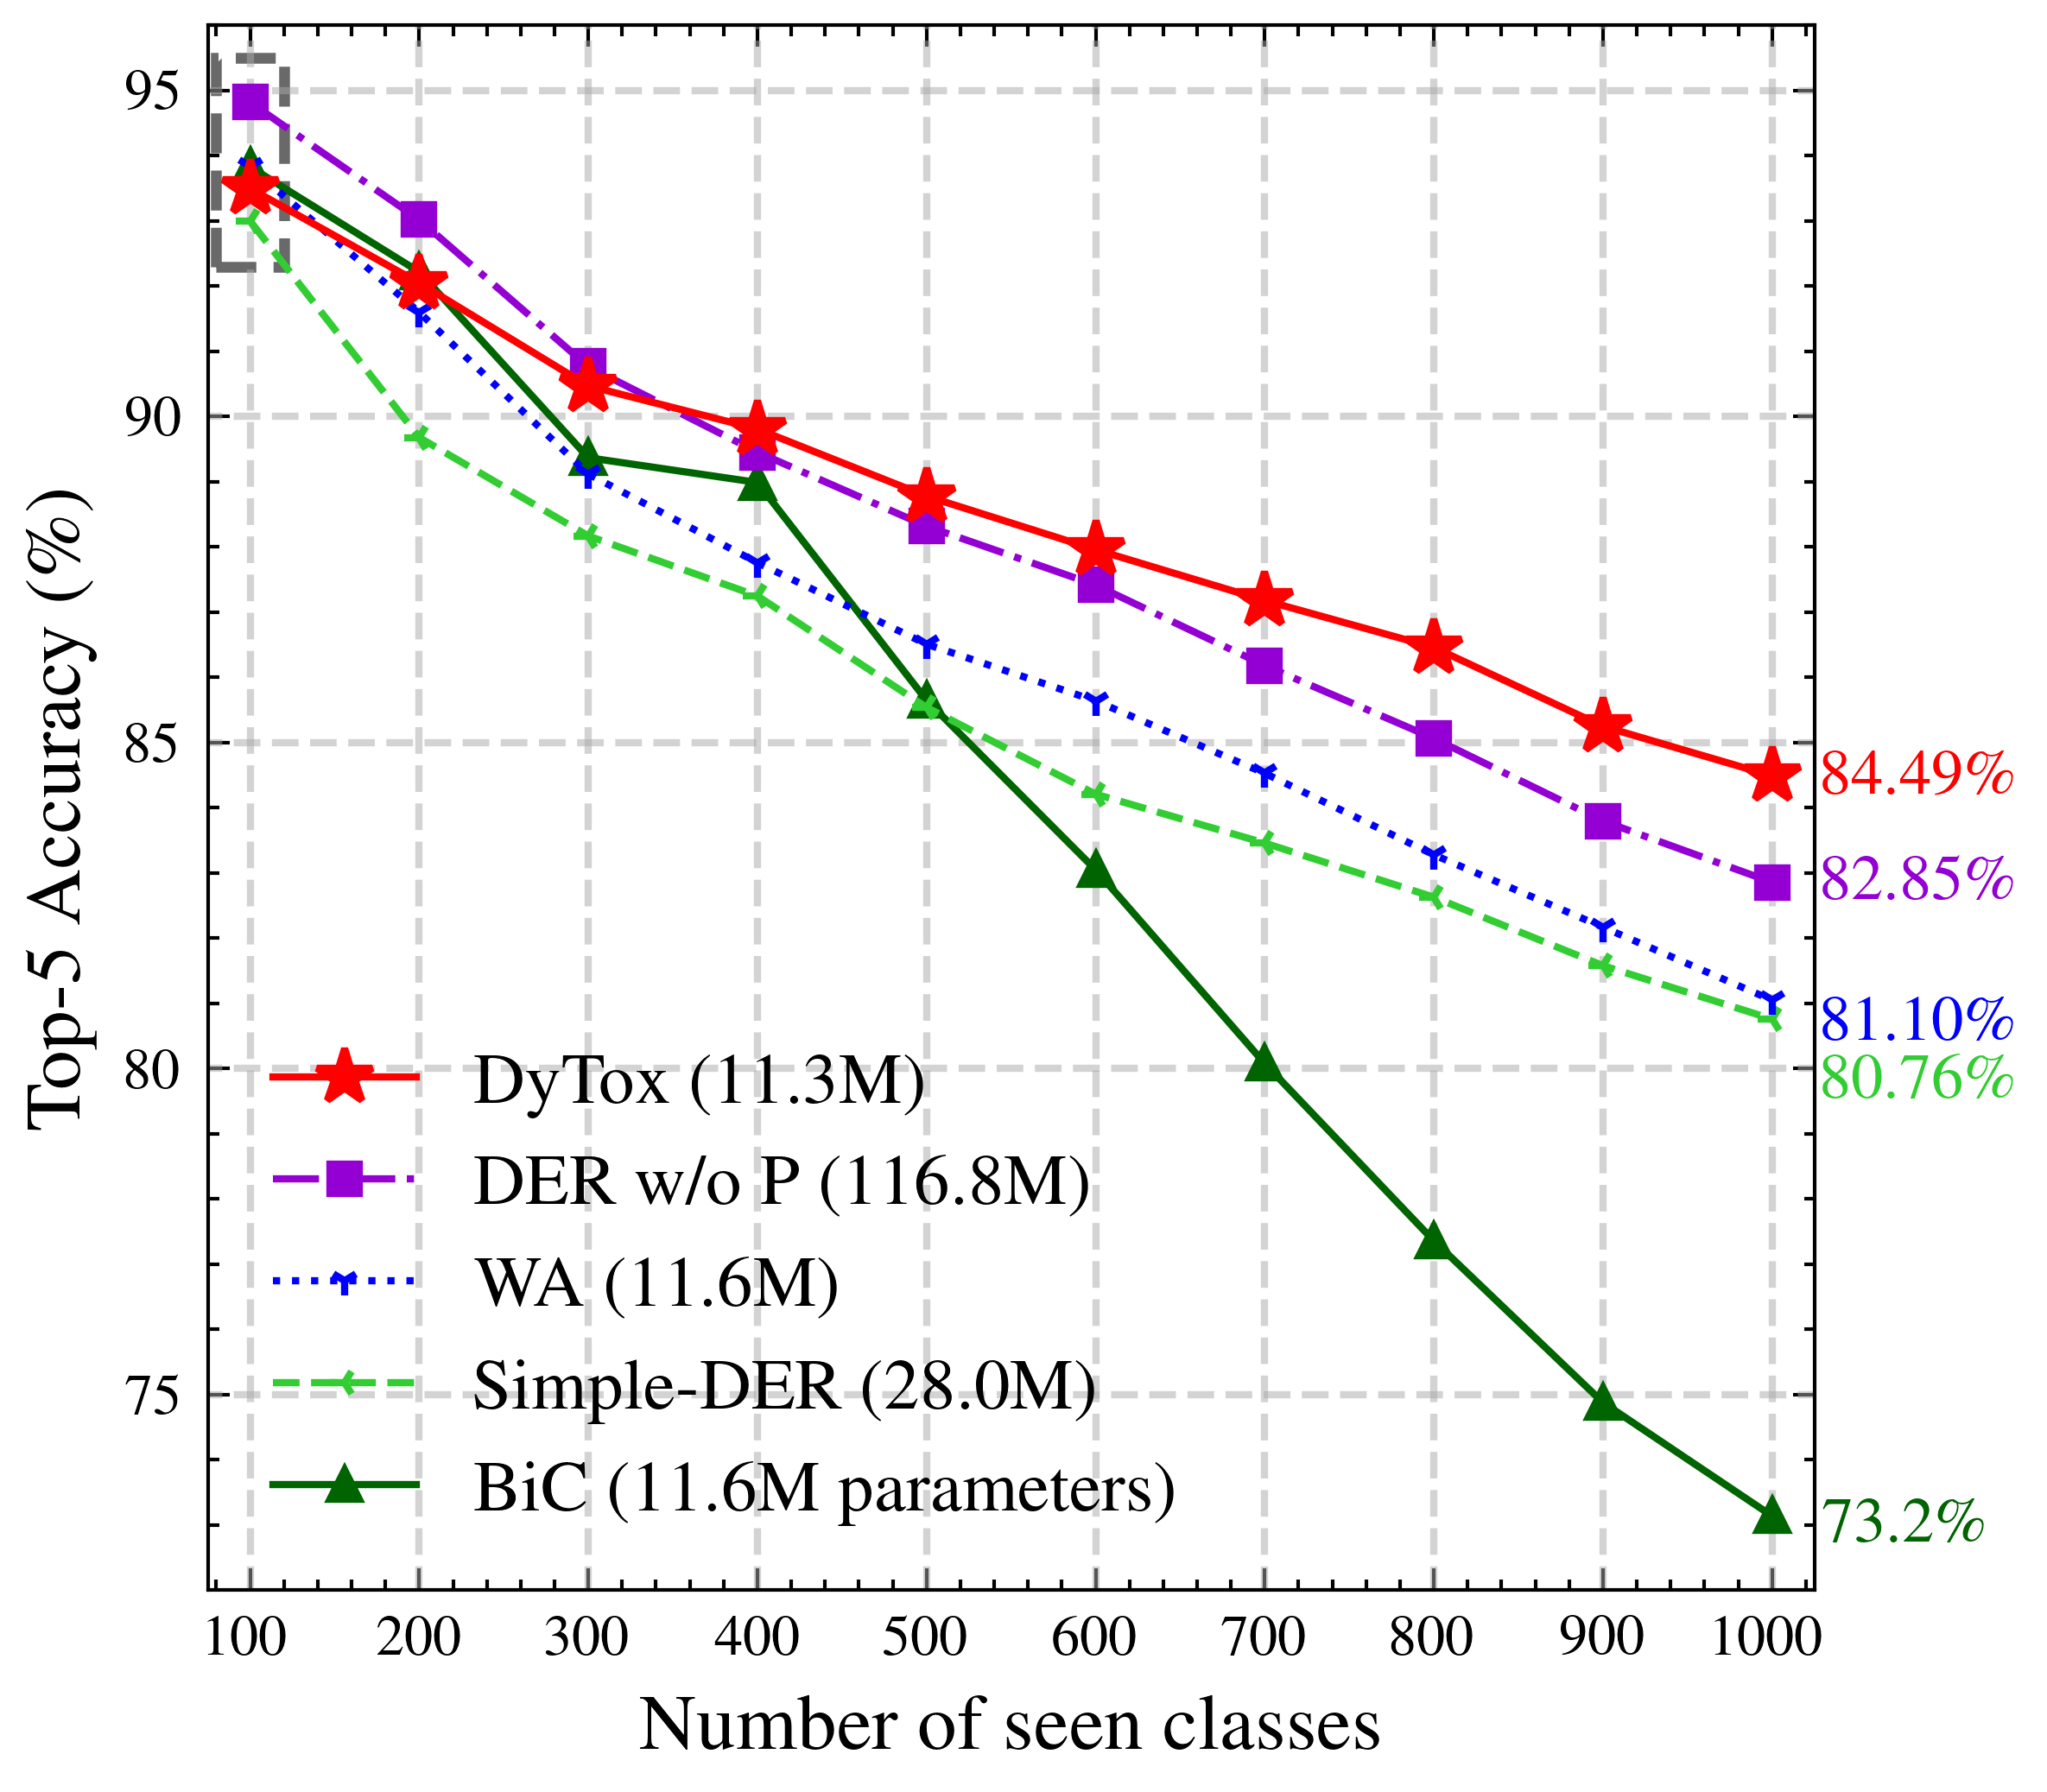
\includegraphics[width=0.9\textwidth]{images/dytox/imagenet1000.png}
        \caption{\textbf{ImageNet1000}}
        \label{fig:dytox_imagenet1000}
    \end{subfigure}%
    \begin{subfigure}{.5\textwidth}
        \centering
        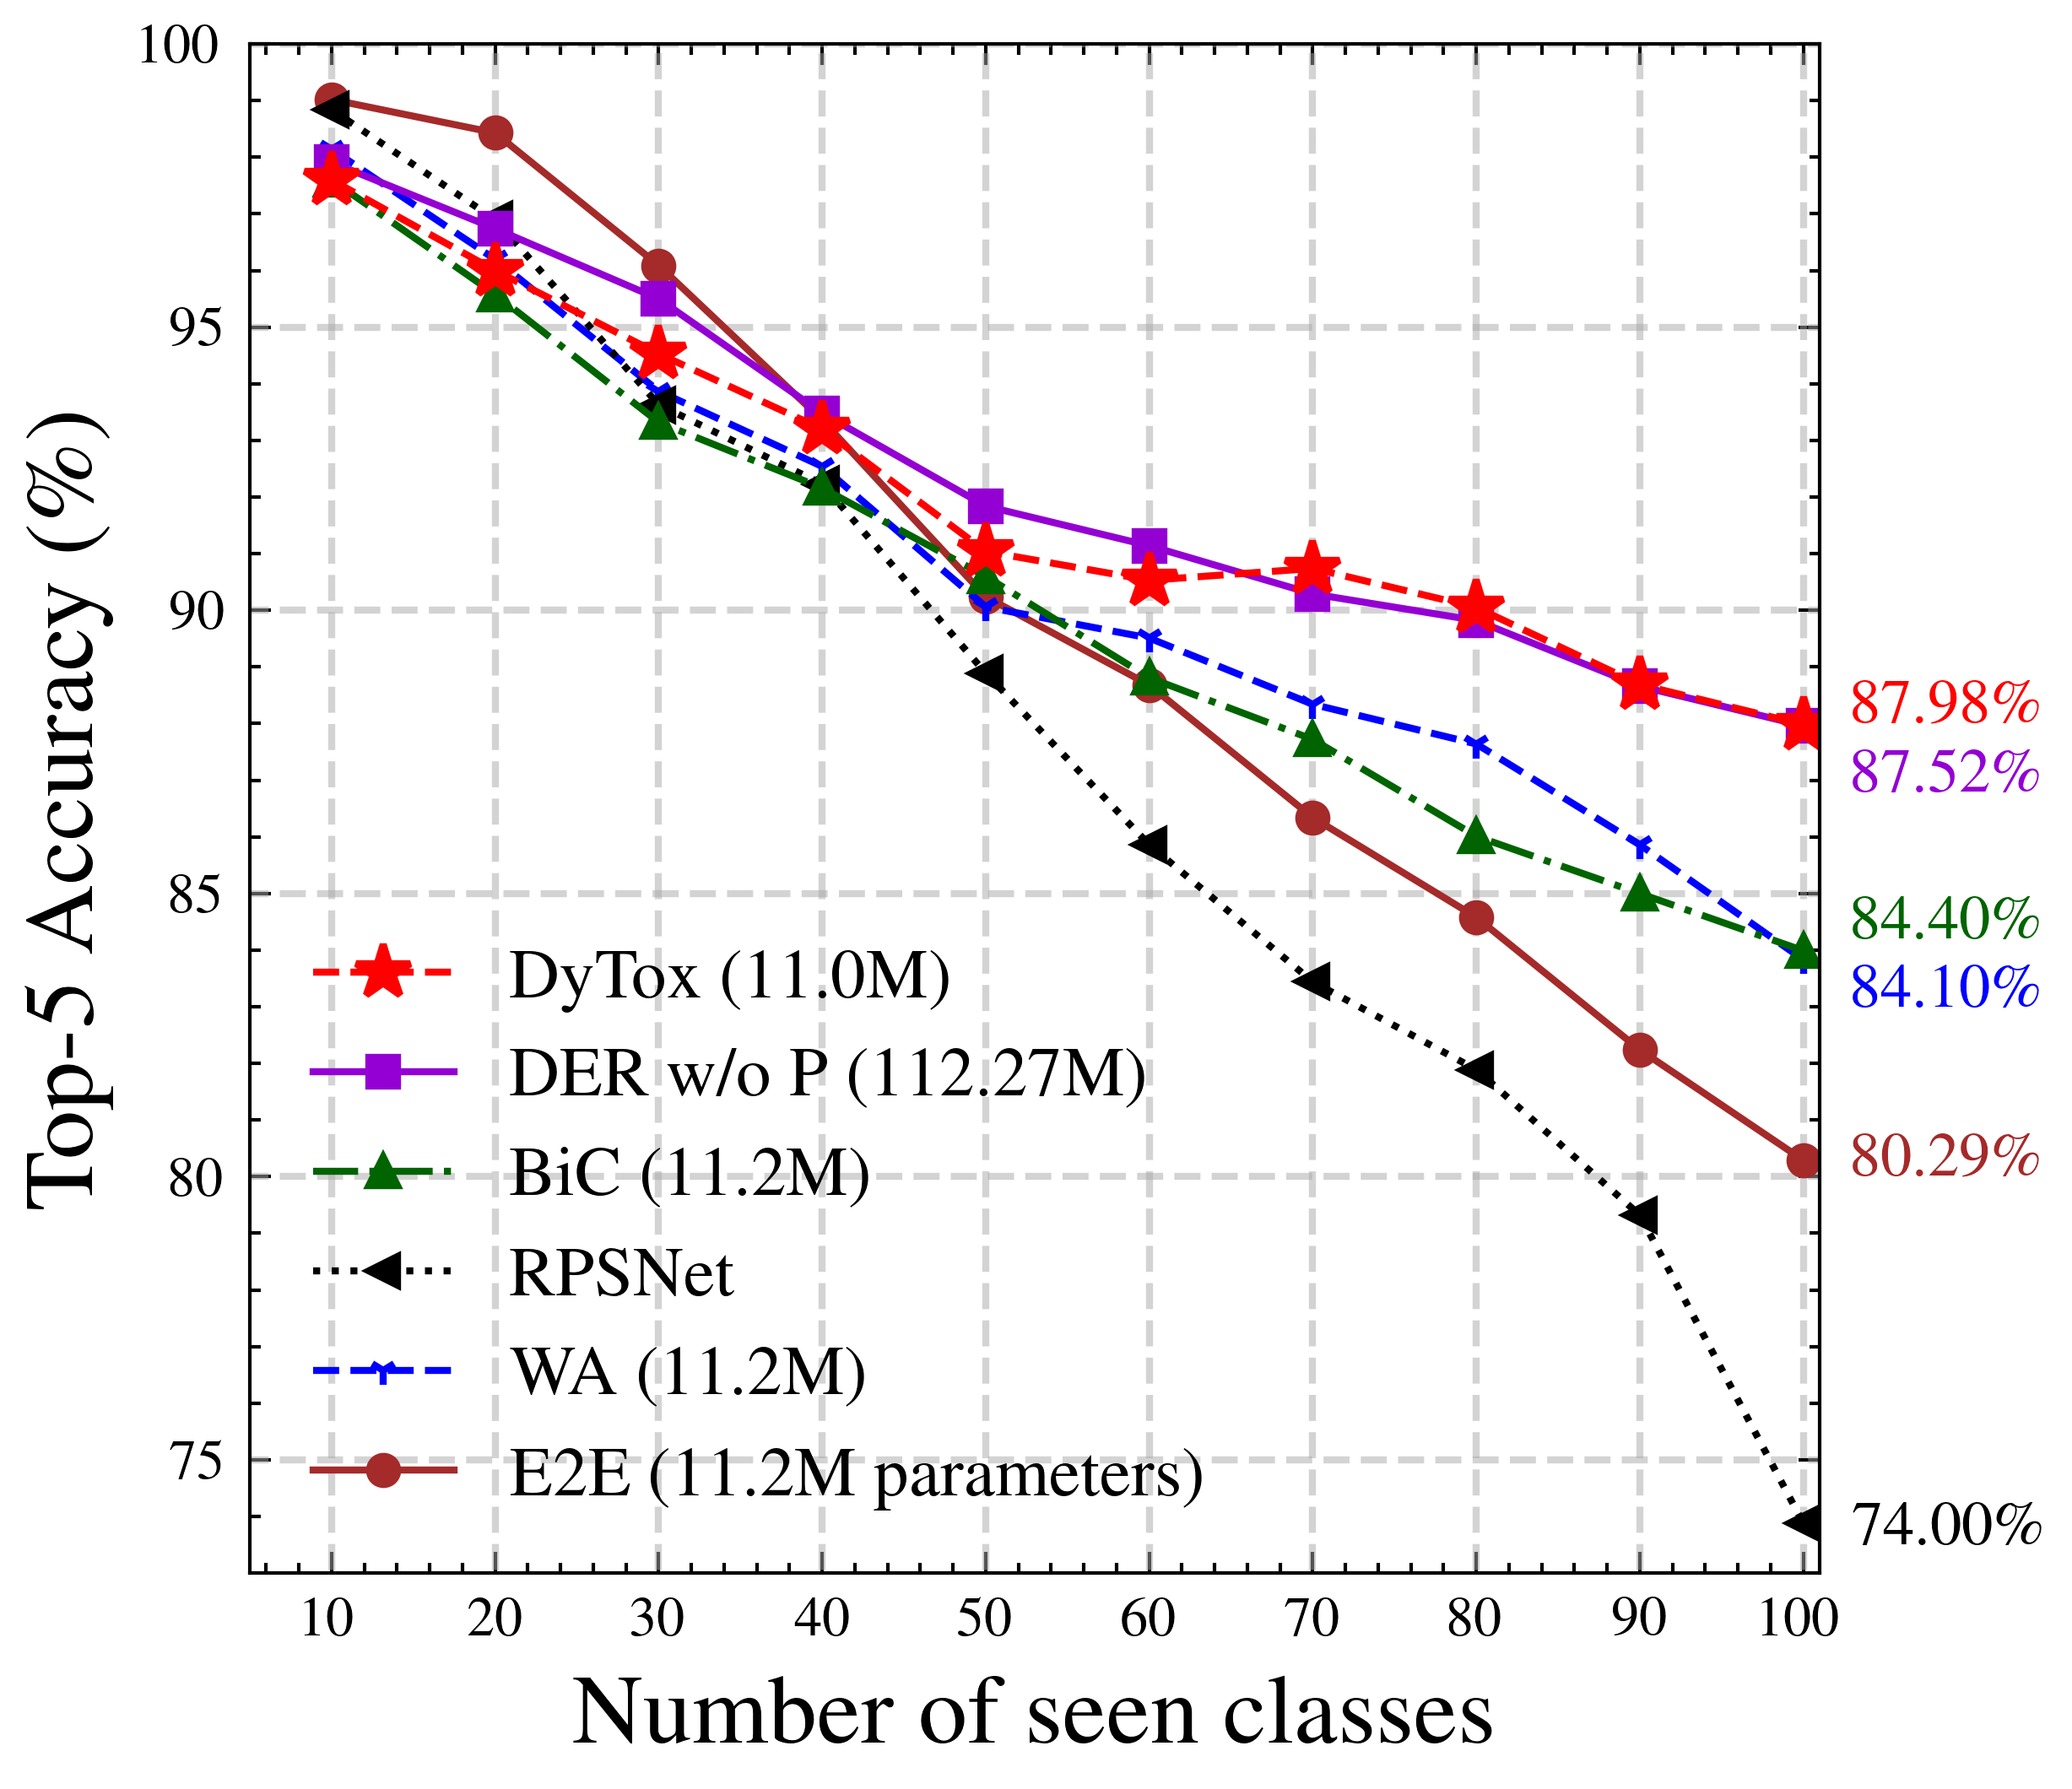
\includegraphics[width=0.9\textwidth]{images/dytox/imagenet100.png}
        \caption{\textbf{ImageNet100}}
        \label{fig:dytox_imagenet100}
    \end{subfigure}
    \caption{\textbf{Performance evolution on ImageNet-\{100, 1000\}.} The top-5 accuracy (\%) is
        reported after learning each task. Our model DyTox (in \textbf{\textcolor{red}{red}}) reaches
        state-of-the-art performance while using significantly fewer parameters than concurrent models.
        Note that at the initial step before the continual process begins, our model has performance
        comparable to other baselines: the performance gain is achieved by reducing catastrophic
        forgetting.}
    \label{fig:dytox_imagenet}
\end{figure}


\subsection{Quantitative results}

\paragraph{ImageNet}
We report performances in \autoref{tab:dytox_imagenet} and in \autoref{tab:dytox_imagenet_pp} for
respectively the ImageNet-1000 and ImageNet-100 dataset. The $^\dagger$
marks the DER with setting-specific pruning, and DER w/o P is for the DER without pruning.
Critically, on the larger-scale ImageNet1000, DyTox systematically performs best on all
metrics despite having lower parameters count. Specifically, DyTox reaches 71.29\% in ``Avg'' top-1
accuracy, and 63.34\% in ``Last'' top-1 accuracy. This outperforms the previous state-of-the-art DER
w/o P (68.84\% in ``Avg'', 60.16\% in ``Last'') which has 10 ResNet18 in parallel and 116.89M
parameters. Compared to the pruned DER$^\dagger$, DyTox has a +4.56 \pp in top-1 and a +1.51 \pp in
top-5 for the ``Avg'' accuracy. In ImageNet100, DyTox reaches 69.10\% and outperforms DER$^\dagger$ by +3.04 percentage points (\pp) in
``Last'' top-1 accuracy. Though, DyTox and DER w/o P somehow perform similarly in ``Avg'' accuracy,
DyTox+ and DyTox++ reach state-of-the-art performance. Specifically, DyTox++, using our full
improved continual training procedure, improves the ``Avg'' top-1 accuracy of DER by 3.58 \pp.

All models evolutions on ImageNet-1000 and ImageNet-100 are illustrated in
\autoref{fig:dytox_imagenet}: DyTox constantly surpasses previous state-of-the-art models --- despite
having a comparable performance at the first step and fewer parameters.

\begin{table*}[t]
    \centering
    \resizebox{1.0\textwidth}{!}{%
        \begin{tabular}{@{}l|ccc|ccc|ccc}
            \hline
                                                                     & \multicolumn{3}{c}{10 steps} & \multicolumn{3}{c}{20 steps}                  & \multicolumn{3}{c}{50 steps}                                                                                                                                                                                                                   \\
            \textbf{Methods}                                         & \textbf{\#P}                 & \textbf{Avg}                                  & \textbf{Last}                & \textbf{\#P}        & \textbf{Avg}                                  & \textbf{Last}                    & \textbf{\#P}        & \textbf{Avg}                                  & \textbf{Last}                    \\
            \hline
            ResNet18 Joint                                           & 11.22                        & -                                             & 80.41                        & 11.22               & -                                             & 81.49                            & 11.22               & -                                             & 81.74                            \\
            Transf. Joint                                            & 10.72                        & -                                             & 76.12                        & 10.72               & -                                             & 76.12                            & 10.72               & -                                             & 76.12                            \\
            \hline
            iCaRL \cite{rebuffi2017icarl}                            & 11.22                        & 65.27\scriptsize{\mypm1.02}                   & 50.74                        & 11.22               & 61.20\scriptsize{\mypm0.83}                   & 43.75                            & 11.22               & 56.08\scriptsize{\mypm0.83}                   & 36.62                            \\
            UCIR \cite{hou2019ucir}                                  & 11.22                        & 58.66\scriptsize{\mypm0.71}                   & 43.39                        & 11.22               & 58.17\scriptsize{\mypm0.30}                   & 40.63                            & 11.22               & 56.86\scriptsize{\mypm0.83}                   & 37.09                            \\
            BiC \cite{wu2019bias_correction}                         & 11.22                        & 68.80\scriptsize{\mypm1.20}                   & 53.54                        & 11.22               & 66.48\scriptsize{\mypm0.32}                   & 47.02                            & 11.22               & 62.09\scriptsize{\mypm0.85}                   & 41.04                            \\
            WA \cite{zhao2020weightalignement}                       & 11.22                        & 69.46\scriptsize{\mypm0.29}                   & 53.78                        & 11.22               & 67.33\scriptsize{\mypm0.15}                   & 47.31                            & 11.22               & 64.32\scriptsize{\mypm0.28}                   & 42.14                            \\
            PODNet \cite{douillard2020podnet}                        & 11.22                        & 58.03\scriptsize{\mypm1.27}                   & 41.05                        & 11.22               & 53.97\scriptsize{\mypm0.85}                   & 35.02                            & 11.22               & 51.19\scriptsize{\mypm1.02}                   & 32.99                            \\
            RPSNet \cite{rajasegaran2019rpsnet}                      & 56.5\,\,                     & 68.60                                         & 57.05                        & -                   & -                                             & -                                & -                   & -                                             & -                                \\
            DER \small{w/o P} \cite{yan2021der}                      & 112.27                       & 75.36\scriptsize{\mypm0.36}                   & \textbf{65.22}               & 224.55              & 74.09\scriptsize{\mypm0.33}                   & 62.48                            & 561.39              & 72.41\scriptsize{\mypm0.36}                   & 59.08                            \\ % no pruning
            \textcolor{gray}{$\text{DER}^\dagger$} \cite{yan2021der} & \textcolor{gray}{-}          & \textcolor{gray}{74.64\scriptsize{\mypm0.28}} & \textcolor{gray}{64.35}      & \textcolor{gray}{-} & \textcolor{gray}{73.98\scriptsize{\mypm0.36}} & \textcolor{gray}{\textbf{62.55}} & \textcolor{gray}{-} & \textcolor{gray}{72.05\scriptsize{\mypm0.55}} & \textcolor{gray}{\textbf{59.76}} \\
            \hline
            DyTox                                                    & 10.73                        & 73.66\mysmpm{0.02}                            & 60.67\mysmpm{0.34}           & 10.74               & 72.27\mysmpm{0.18}                            & 56.32\mysmpm{{0.61}}             & 10.77               & 70.20\mysmpm{0.16}                            & 52.34\mysmpm{0.26}               \\
            DyTox+                                                   & 10.73                        & \textbf{75.54}\mysmpm{0.10}                   & 62.06\mysmpm{0.25}           & 10.74               & \textbf{75.04}\mysmpm{0.11}                   & 60.03\mysmpm{0.45}               & 10.77               & \textbf{74.35}\mysmpm{0.05}                   & 57.09\mysmpm{0.13}               \\
            \hline
        \end{tabular}
    }
    \caption{\textbf{Results on CIFAR100} averaged over three different class orders. Baselines
        results are come from \cite{yan2021der}. The $\dagger$ symbol means that \cite{yan2021der}
        needed setting-sensitive hyperparameters. Moreover, its reported parameters count was an average
        over all steps: the final parameters count (necessarily higher) was not available.}
    \label{tab:dytox_cifar100-b0}
\end{table*}


\begin{figure*}[t!]
    \centering
    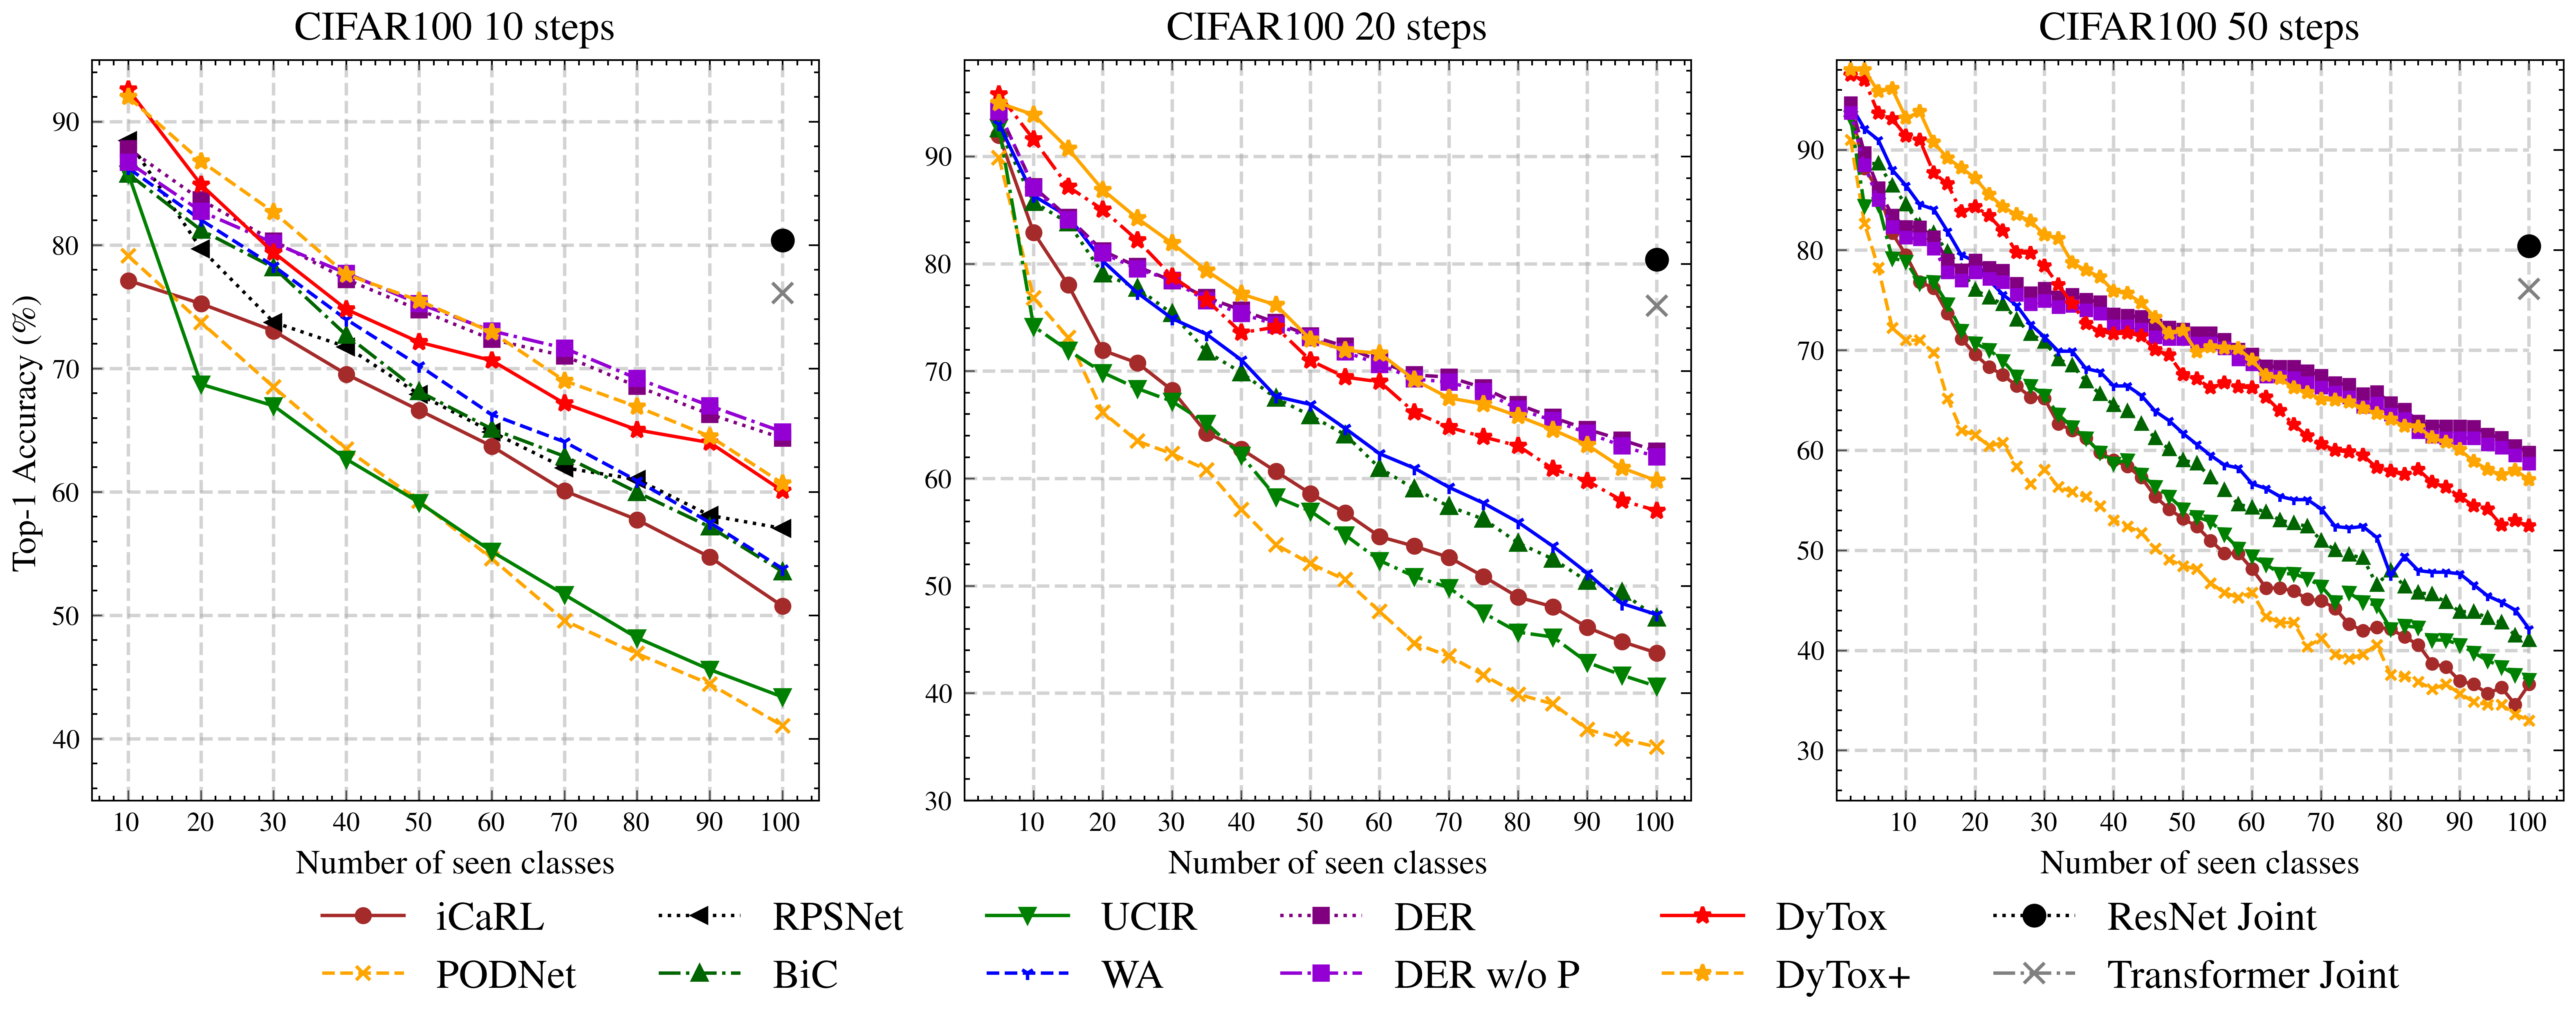
\includegraphics[width=1.0\linewidth]{images/dytox/cifar.png}
    \caption{\textbf{Performance evolution on CIFAR100}. The top-1 accuracy (\%) is reported after
        learning each task. \textbf{Left} is evaluated with 10 steps, \textbf{middle} with 20 steps, and
        \textbf{right} with 50 steps.}
    \label{fig:dytox_increment_cifar}
\end{figure*}

DyTox is able to scale correctly while handling seamlessly the parameter growth by sharing most of
the weights across tasks. In contrast, DER had to propose a complex pruning method; unfortunately,
this pruning required different hyperparameter values for different settings. Despite this, the
pruning in DER$^\dagger$ is less efficient when classes diversity increase: DER$^\dagger$ doubles in
size between ImageNet100 and ImageNet1000 (\citet{yan2021der} report 7.67M \textit{vs.} 14.52M)
while handling the same amount of tasks (10). Note that these parameter counts reported for
DER$^\dagger$ in \citet{yan2021der} are in fact averages over all steps: the final parameters count
(necessarily higher) was not available and thus is not reported in our tables. Simple-DER also
applies pruning but without hyperparameter tuning; while simpler, the pruning is also less efficient
and induces larger model (28.00M parameters).

%\vspace{-0.5em}
\paragraph{CIFAR100} \autoref{tab:dytox_cifar100-b0} shows results for all approaches on CIFAR100.
The more steps there are, the larger the forgetting is and thus the lower the performances are.
Those settings are also displayed in \autoref{fig:dytox_increment_cifar} after each task. In every
setting, DyTox is close to DER w/o P  for much fewer parameters (up to 52x less). Critically, DyTox
is significantly above other baselines: \eg DyTox is up to +25\% in ``Last'' accuracy in the 50
steps setup. Note that our improved continual training procedure, with DyTox+ and DyToX++, further
increases the results in all settings. Notably DyTox++ increases the ``Àvg'' accuracy in the 50
setup over DER by +3.4 \pp. Remark also that DER ``Avg'' accuracy degrades by 2.59 \pp between the
easiest 10 steps setting and the hardest 50 steps setting. In comparison, DyTox++ only loses 1.65
\pp, proving a better robustness to forgetting as the number of tasks increases. Remark that the
results in this table of our PODNet, presented in \autoref{chapter:regularization}, can be explained
because of the slightly different setting: PODNet was designed for situation where half of the
dataset's classes were learned in a single step, and thus providing a better initialization. PODNet,
a metric-based model (as also UCIR), excelled in those situations, but struggle when the initial
step contains few classes (as it is the case in this chapter) due to slower initial learning.
Arguably, in a real-life scenario, a model should be pretrained on a large dataset and therefore
this ``\textit{weakness}'' of PODNet won't materialize.

\subsection{Model introspection on CIFAR100}

\paragraph{Memory overhead}
We only add a vector of size $d=384$ per task; thus, the overhead in memory (not considering the
growing classifier which is common for all continual models) is only of $+0.004\%$ per step. Even in
the challenging setting of CIFAR100 with 50 tasks, our memory overhead is almost null ($+0.2\%$).

\label{sec:dytox_comp_over}
%\vspace{-1em}
\paragraph{Computational overhead} The vast majority of the computation is done in the SABs, thus
shared among all tasks. The dynamical component of our model is located at the ultimate TAB.
Moreover, the Task-Attention, contrary to the Self-Attention, has a time complexity linear in terms
of tokens and not quadratic reducing the time overhead to an acceptable sub-linear amount. Overall,
for each new task, one forward pass is only $2.24\%$ slower than at the previous task.
Furthermore, the procedure can be accelerated by doing a single forward pass through the TAB with
a masked attention \citep{vaswani2017transformer}: the query is the concatenation of all task
tokens, then we mask the attention logits corresponding to an interaction between task tokens. For
an almost equivalent result (modulo numerical imprecision), a new task only increases the time spent
in a forward pass by $1.09\%$.

%\vspace{-1em}
\begin{table}[t]
    \centering
    \begin{tabular}{@{}l|c|ccc}
        \hline
                          & Joint (1 step)                                  & \multicolumn{2}{c}{50 steps}                                                                             \\
        \textbf{Training} & \textbf{Last} ($\uparrow$)                      & \textbf{Last} ($\uparrow$)                      & \textbf{Forgetting} ($\downarrow$)\Tstrut\Bstrut       \\
        \hline
        DyTox             & 76.12                                           & 52.34                                           & 33.15 \Tstrut                                          \\
        DyTox+            & 77.51\scriptsize{\textcolor{OliveGreen}{+1.39}} & 57.09\scriptsize{\textcolor{OliveGreen}{+4.75}} & 31.50\scriptsize{\textcolor{OliveGreen}{-1.65}}\Bstrut \\
        DyTox++           & 77.91\scriptsize{\textcolor{OliveGreen}{+0.40}} & 58.76\scriptsize{\textcolor{OliveGreen}{+1.67}} & 30.47\scriptsize{\textcolor{OliveGreen}{-1.03}}        \\
        \hline
    \end{tabular}
    \caption{\textbf{``Last'' accuracy and forgetting} \cite{chaudhry2018riemannien_walk} on
        CIFAR100 for the joint (1 step, no continual) and 50 steps settings.}
    \label{tab:dytox_training_plus}
\end{table}


\paragraph{Training procedure introspection} Our DyTox+ and DyTox++ strategies really reduce
catastrophic forgetting and does not just improve raw performances. This is shown in
\autoref{tab:dytox_training_plusplus}, where we compare DyTox \vs DyTox+ \vs DyTox++ strategies on
CIFAR100. In the joint setting, our model slightly benefits from both MixUp and ASAM: the gain is
limited (+1.79 \pp). On the other hand, those two methods greatly improve the extreme
continual setting of 50 steps (+6.42 \pp). This shows that the gain is not due to absolute
improvements of the model performance. Moreover, using the forgetting measure of
\citet{chaudhry2018riemannien_walk}, we compare how much a model has forgotten relatively to its
previous tasks. This metric is therefore agnostic to absolute performance improvements. DyTox had a
forgetting of 33.15\%, DyTox+ of 31.50\%, and DyTox++ of 30.47\%: a total reduction of 2.68 \pp.
This validates our novel training procedures that are particularly efficient for continual learning.
The computational overhead of ASAM is lower than more complex second-order methods, but it still
doubles the number of forward and backward passes. For this reason, we didn't evaluated DyTox++ on
the large ImageNet1000. However, future works could consider the promising Look-SAM
\cite{liu2021looksam} to reduce the time overhead.

\begin{table}
    \centering
    \begin{tabular}{ll|ccccc|cc}
         &                                                                                               & \rot{\footnotesize{Knowledge Distillation}} & \rot{\footnotesize{Finetuning}} & \rot{\footnotesize{Token Expansion}} & \rot{\footnotesize{Divergence Classifier}} & \rot{\footnotesize{Indendepent Classifiers}} & \textbf{Avg} & \textbf{Last} \\
        \hline
        \parbox[t]{2mm}{\multirow{7}{*}{\rotatebox[origin=c]{90}{\textbf{DyTox}}}}
         & \parbox[t]{3mm}{\multirow{3}{*}{\rotatebox[origin=c]{90}{\textbf{\scriptsize{Transformer}}}}}
         &                                                                                               &                                             &                                 &                                      &                                            & 60.69                                        & 38.87\Tstrut                 \\
         &                                                                                               & \cmark                                      &                                 &                                      &                                            &                                              & 61.62        & 39.35         \\
         &                                                                                               & \cmark                                      & \cmark                          &                                      &                                            &                                              & 63.42        & 42.21         \\[3pt]
        %\vspace{0.01cm}
        \cline{2-9}
         & \parbox[t]{3mm}{\multirow{3}{*}{\rotatebox[origin=c]{90}{\textbf{\scriptsize{Dynamic}}}}}
         & \cmark                                                                                        & \cmark                                      & \cmark                          &                                      &                                            & 67.30                                        & 47.57\Tstrut                 \\
         &                                                                                               & \cmark                                      & \cmark                          & \cmark                               & \cmark                                     &                                              & 68.28        & 49.45         \\
         &                                                                                               & \cmark                                      & \cmark                          & \cmark                               & \cmark                                     & \cmark                                       & 70.20        & 52.34\Bstrut  \\
        \hline
    \end{tabular}
    \caption{\textbf{Ablations} of the different key components of our DyTox architecture. We report
    the average accuracy and the last accuracy on CIFAR100 for the setting with 50
    steps.\vspace{-1em}}
    \label{tab:dytox_ablation}
\end{table}

\FloatBarrier

%\vspace{-1em}
\label{sec:dytox_ablations}
\paragraph{Model ablations} We ablate the importance of the different components of DyTox in
\autoref{tab:dytox_ablation}. We add on the base transformer a naive knowledge distillation
\citep{hinton2015knowledge_distillation} and a finetuning
\citep{castro2018end_to_end_inc_learn} applied after each
task on a balanced set of new data and rehearsal data. Finally, our DyTox strategy exploits directly
the very nature of transformers (separated task information from the pixels information) to tackle
catastrophic forgetting with three components: (1) a task token expansion, (2) a divergence
classifier, and (3) independent classifiers. All three greatly improve over the baseline transformer
($42.21\% \rightarrow 52.34\%$ in ``Last'') while having almost no memory overhead ($+0.2\%$). The
divergence classifier improves the diversity between task tokens: we observed that the minimal
Euclidean distance between them increases by 8\%. Moreover, we also remarked that having independent
classifiers reduces the forgetting defined by \citet{chaudhry2018riemannien_walk} by more than
24\%.


\section{Conclusion}

In this chapter, we covered our work on dynamic architectures. While in previous chapters, we aimed
to constrain the visual features, we decided here to condition the features to specific tasks. With
DyTox, a new dynamic strategy for continual learning based on transformer architecture, all tasks
share a common encoding produced by self-attention layers. Then, task-specific tokens are used to
produce task-specialized embeddings through a new task-attention layer. This architecture allows
to dynamically process new tasks with very little memory overhead and does not require complex
hyperparameter tuning. Our experiments show that our framework scales to large datasets and an
important number of tasks efficiently while using significantly fewer parameters than concurrent
dynamic strategies.

\cleardoublepage
\let\leftmark=\oldleftmark

\acresetall
\chapter{Spaced Repetition against Forgetting}
\label{chapter:spacedrepet}

%\minitoc
\chapterwithfigures{\nameref*{chapter:spacedrepet}}
%\chapterwithtables{\nameref*{chapter:introduction}}

\ifthenelse{\boolean{skipRepet}}{\endinput}{}

\section{Introduction}

\section{Anki}

\subsection{Model}

\subsection{Experiment results}

\section{Conclusion}


\cleardoublepage
\let\leftmark=\oldleftmark

\acresetall
\chapter{Conclusion}
\label{chapter:conclusion}

%\minitoc
\chapterwithfigures{\nameref*{chapter:conclusion}}
%\chapterwithtables{\nameref*{chapter:introduction}}

\ifthenelse{\boolean{skipConclusion}}{\endinput}{}

We now summarize the contributions of this thesis and offer some future directions of Continual
Learning.

\section{Contributions}

During this thesis, we aim to learn an increasing number of classes with \ac{DL} architectures for
\ac{CV} without forgetting. We design multiple methods to achieve this goal, with a particular
interest on how the visual features of a continual model evolve through time. First, in
\autoref{chapter:regularization}, we investigate how to constrain features while satisfying a
rigidity-plasticity trade-off. Then, in \autoref{chapter:segmentation}, we explore continual
approaches for semantic segmentation. Finally, in \autoref{chapter:dynamic}, we exploit the
transformer architecture in a dynamic framework to condition features per task.

\paragraph{Visual Features regularization} We study in \autoref{chapter:regularization} \ac{CIL} for
image classification. In this setting, regularization constraining a model's output is the most
common approach. We challenge this paradigm by outlining two drawbacks: it balances poorly the
rigidity (not forgetting old classes) \vs plasticity (learning new classes) trade-off. Moreover,
constraining intermediary visual features is a stronger regularization. Then, we design two
feature-based regularizations: (1) PODNet minimizes the drift between statistics of the visual
features between the old and new models. The design of this method explicitly reduces forgetting
while letting enough slack to efficiently learn new classes. (2) Our second approach, Ghost, avoids
forgetting before it even happens by pre-allocating areas of the latent space for future classes by
drawing inspiration from the zeroshot literature. For this second approach, we propose the Prescient
Continual Learning setting where detailed attributes of each class are available. This is a
reasonable assumption in the fashion context of Heuritech, the company sponsoring this PhD.

\paragraph{Continual Semantic Segmentation} We explore \ac{CSS} in \autoref{chapter:segmentation}.
We highlight the two main challenges: an important catastrophic forgetting linked to the higher
complexity of segmentation images, and a background shift where only classes of the current task are
labeled. To reduce the catastrophic forgetting of old classes, inspired by our previous POD, we
present a multi-scale distillation loss that constrains local regions of visual features. Then, to
tackle the background shift, we design an uncertainty-based hard pseudo-labeling loss. We show that
despite its usefulness, our pseudo-labeling can fail for particular situations, and complement it
with an efficient object rehearsal method.

\paragraph{Dynamic Strategy with Transformers} Finally, in \autoref{chapter:dynamic}, we propose to
use the recent transformer architecture with a dynamic strategy in \acf{CIL} for image
classification. Previous dynamic networks, that expand their parameters as the number of learned
tasks increases, struggle to limit their memory and time overheads. We propose instead to share a
common encoding produced by self-attention layers, and to condition the features for each task using
task-specific tokens. This architecture allows us to dynamically process new tasks with very little
memory overhead even when faced to a large number of tasks.

\section{Future Work}

We now discuss some future directions of our work, both with respect to the data/benchmark and to
the architecture/optimization process.

\vspace{2em}
\noindent{\large{\textbf{Data \& Benchmarks}}}

\paragraph{Time Limitation} Current works in the literature, including this thesis, focus on using
no rehearsal data or at least very few. The common justifications are about private data that cannot
be kept, or embedded device with little storage. In many situations, those constraints are
realistic. However, in other situations, given large data centers, storage capacity is less a
problem. In that case, the main constraint is time: continually learn new data should be
significantly faster than retraining from scratch. Thus, a new setting with large-scale rehearsal
memory for continual learning would impose a time budget \citep{veniat2018budgetedlearning}.

\paragraph{Universal Representation} A major cause of forgetting in deep neural networks is that
they learn spurious features \citep{lesort2022spuriousfeatures}, useful for the current task, but
that may cause interference with future tasks. Ideally, a network should learn invariants
\citep{arjovsky2019irm,rame2021fishr} that generalizes better to new distributions. Recently, it has
been proposed that self-supervision could learn more class-agnostic features and in turns
drastically reduce forgetting \citep{gallardo2021selfsupcontinual}. Universal
features, trained in self-supervision, with a metric-based approach, on a wide diversity of
modalities (RGB, depth, \etc), will enable better continual models. First, they would forget less
because the need to adapt the representation to new tasks is reduced. Second, an adaptation to new
tasks will be extremely quick, where simply tuning a task token in a Dytox-like strategy would
result in good performances.

\vspace{2em}
\noindent{\large{\textbf{Architecture \& Optimization}}}

\paragraph{Deep Architectures} for continual learning is a fewly explored topic as most works focus
on a fixed MLP or a ResNet-18. Initial findings remark that larger networks forget less
\citep{ramasesh2022scalecontinual}, especially when scaling the width
\citep{mirzadeh2022widecontinualnetworks}. Going further than simply scaling, one may wonder if the
structure of current architectures, optimized for \iid training, have inherent flaws regarding
continual learning. More particularly, Mixture-of-Experts (MoE) is an interesting direction for
continual learning \citep{caccia2022anytimelearning}: large models could learn universal features
that could be conditioned with task-specific experts. The usage of experts does not necessarily need
to be exclusive to a particular task: in fact a form of compositionality could be obtained where
each expert specializes a some concept. This compositionality could speed up the learning of new
tasks with little forgetting without requiring an important adaptation of the parameters.

\paragraph{Second-order optimization} methods can help deep neural networks to find wide local
minima, which could encompass multiple task local minima \citep{lee2020kroneckercontinual}. As a
result, the parameter drift between the optimal weights of a task $t$ and $t+1$ can be minimal, and
in turn avoid the bulk of the forgetting. We briefly explore this direction with the
Sharpness-Aware-Minimizer \citep{foret2020sam} in this thesis, but more work could be done on this
topic. An important drawback of current second-order methods is obviously the higher computational
cost they incur, thus faster alternative methods also seeking flat wide minima such as
\citet{cha2021swad}'s SWAD could be explored.

\paragraph{Learning differently} The vast majority of deep architectures, in all domains, are
trained with gradient descent (including fancier optimizers as Adam or LAMB). The major drawback of
this update rule is the ``\textit{tug-of-war}'' \citep{hadsell2020embracingchange} where the
gradient from each task pulls the solution towards its optimum. Different update rules, more closely
inspired from the biological brains, can be an axis of investigation, as Hebbian learning for
continual learning \citep{taylor2020hebbiancontinual}. Moreover, instead of designing explicitly an
update rule, it could be meta-learned. This meta-learning could aim faster remembering of previous
forgotten tasks \citep{he2019metacontinual,caccia2020osaka}.



\cleardoublepage
\let\leftmark=\oldleftmark

\acresetall
\chapter{Appendix: more papers}
\label{chapter:appendix}

%\minitoc
\chapterwithfigures{\nameref*{chapter:appendix}}
%\chapterwithtables{\nameref*{chapter:introduction}}

\ifthenelse{\boolean{skipAppendix}}{\endinput}{}

\section{Details on PODNet}
\label{sec:appendix_podnet}

\subsection{Implementation details}

For all datasets, images are augmented with random crops and flips. For CIFAR100, we additionally
change image intensity by a random value in the range [-63, 63].
%
We train our model for 160 epochs for CIFAR100, and 90 epochs for both ImageNet100 and ImageNet100,
with a SGD optimizer with momentum of 0.9. For all datasets, we start with a learning rate of 0.1, a
batch size of 128, and cosine annealing scheduling.
%
The weight decay is $5\cdot 10^{-4}$ for CIFAR100, and $1\cdot 10^{-4}$ for ImageNet100 and
ImageNet1000. For CIFAR100 we set model hyperparameters $\lambda_c = 3$ and $\lambda_f=1$, while for
ImageNet100 and 1000 we set $\lambda_c = 8$ and $\lambda_f =10$. Our model uses POD-spatial and
POD-flat except when explicitly stated otherwise. Following Hou et al.~\cite{hou2019ucir}, we
multiply both losses by the adaptive scaling factor: $\lambda=\sqrt{\nicefrac{N}{T}}$ with $N$ being
the number of seen classes and $T$ the number of classes in the current task.

For POD-spatial, before sum-pooling we take the features to the power of 2 element-wise. The vector
resulting from the pooling is then L2 normalized.

\subsection{Number of proxies per class}

While our model's expressiveness increases with more proxies in $\mcL_\text{LSC}$, it remains fairly
stable for values between 5 and 15, thus, for simplicity, we kept it fixed to 10 in all experiments.

In initial experiments, we had the following pairs for the number of clusters (k) and average
incremental accuracy (acc): k=1, acc=56.80\%; k=2, 57.14\%; k=4, acc=57.40\%; k=6, acc=57.46\%; k=8,
acc=57.95\%, and k=10, acc=57.98\% --- i.e., a 1.18 p.p. improvement moving from k=1 to k=10. On
ImageNet100, with 10 steps/tasks (increments of give classes per task), moving from k=1 to k=10
improved 1.51 p.p. on acc.

\subsection{Reproducibility}

\paragraph{Code Dependencies} The Python version is  3.7.6. We used the PyTorch
\cite{paszke2017pytorch} (version 1.2.0) deep learning framework and the libraries Torchvision
(version 0.4.0), NumPy \cite{oliphant2006numpy} (version 1.17.2), Pillow (version 6.2.1), and
Matplotlib \cite{hunter2007matplotlib} (version 3.1.0). The CUDA version is 10.2. Initial
experiments were done with the data loaders library Continuum \cite{douillardlesort2020continuum}.
PODNet's full code is released at:\\
\href{https://github.com/arthurdouillard/incremental\_learning.pytorch}{\texttt{github.com/arthurdouillard/incremental\_learning.pytorch}}.
\\We provide all configuration files necessary to reproduce results, including seeds and class
ordering.

\paragraph{Datasets description} I provide bellow extensive details on the content of the three
datasets considered for PODNet: CIFAR100, ImageNet100, and ImageNet1000.

{\begin{description} \setlength{\parskip}{0pt}
    \item[CIFAR100] contains 32$\times$32-pixel images in 100 classes, with 50k images for training
          and 10k for testing.
    \item[ImageNet100] contains 224$\times$224-pixel images in 100 classes, with $\sim$128k images
          for training and $\sim$5k for testing.
    \item[ImageNet1000] contains 224$\times$224-pixel images in 1000 classes, with $\sim$1.28m
          images for training and $\sim$50k for testing. \end{description}}

\paragraph{Spatial-based distillation} I displayed the differences of performance between
spatial-based distillation in \autoref{sec:podnet_ablation_pooling}
(\autoref{tab:podnet_ablation_perceptual}) when combined with POD-flat. In this appendix, I also
detail in \autoref{tab:podnet_ablation_perceptual_noflat} the same spatial-loss without POD-flat.
The ranking between distillation losses is ostensibly the same. Notice that POD-spatial ---and its
sub-components POD-width and POD-height-- are the only losses barely affected by POD-flat's absence.
Note that all alternative losses were tuned on the validation set to get the best performance,
including those from external papers. Still, our proposed loss, POD-spatial, outperforms all, both
with and without POD-flat.


\begin{table*}[!htbp]
    \centering
    \begin{tabular}{@{}lcc@{}}
        \toprule
        Loss                                                        & NME            & CNN            \\
        \midrule
        \textit{None}                                               & 41.56          & 40.76          \\
        POD-pixels                                                  & 42.21          & 40.81          \\
        POD-channels                                                & 55.91          & 50.34          \\
        POD-gap                                                     & 57.25          & 53.87          \\
        POD-width                                                   & 61.25          & 57.51          \\
        POD-height                                                  & 61.24          & 57.50          \\
        POD-spatial                                                 & \textbf{61.42} & \textbf{57.64} \\
        \hdashline
        GradCam~\citep{dhar2019learning_without_memorizing_gradcam} & 41.89          & 42.07          \\
        Perceptual Style~\citep{johnson2016perceptual_losses}       & 41.74          & 40.80          \\
        \bottomrule
    \end{tabular}
    \caption{\textbf{Comparison of distillation losses} based on intermediary features. All losses evaluated
        without POD-flat. We report the average incremental accuracy on CIFAR100 with 50 steps.}
    \label{tab:podnet_ablation_perceptual_noflat}
\end{table*}



\section{Details on Ghost}
\label{sec:appendix_ghost}


\subsection{Overhead of SVMs training}

Training the SVMs for $\mcL^{\text{\tiny{svm-reg}}}$ introduces a computational overhead. To
minimize it, we limit the number of features per class to 500. Moreover, as we advance towards later
tasks, fewer unseen classes remain, and thus we have fewer SVMs to train. Overall, an experiment on
AwA2, with our setting of 25 classes + 5 $\times$ 5 classes, takes 5 hours to train. We observed
that our SVM-based regularization extends that time by less than 5 minutes on average, an overhead
of less than 2\%, which we deemed acceptable. For reference, the SVMs were trained on a machine with
10 CPU cores of 3.90GHz each.

\subsection{Implementation Details} For all datasets and settings, we set the classification margin
$\delta=0.6$, and the SVM latent-space regularization additional margin $\tau=1$. We train the
feature-extractor-and-classifier pipeline for 90 epochs with an SGD optimizer, learning rate of 0.1,
cosine scheduling, and weight decay of $10^{-4}$. We train the generator for 1200 epochs, with an
Adam optimizer and a learning rate of $10^{-5}$. Finally, following
\cite{hou2019ucir,douillard2020podnet}, we fine-tune the classifier for 60 epochs (with the feature
extractor frozen and a small learning rate of $10^-4$) at the end of every task (except the last
one). We found useful to balance the bias towards the seen classes against the unseen classes. With
the POD distillation \cite{douillard2020podnet}, we set $\lambda_1=3$  for AwA2, and $\lambda_1=15$
for aP\&Y; with the Less-Forget distillation \cite{hou2019ucir}, we set $\lambda_1=4$ for both
datasets. We always set $\lambda_2=10^{-3}$, moreover we apply it on L2-normalized features.
Finally, we do not reinitialize the models between tasks: $f^t$ results from training $f^{t-1}$ on
task $t$, etc. On the rehearsal memory limitation, we follow the strict setting of Hou et
al.~\cite{hou2019ucir}, keeping only $s=20$ training images per past class.

\subsection{Datasets details}

We train our model on three datasets: MNIST, AwA2, and aP\&Y. Baselines and our Ghost models are run
on the exact same data/class splits, with the exact same preprocessing.

\paragraph{MNIST} This dataset has ten classes: handwritten digits ranging from '0'' to '9'. It has
a training set of 60,000 images and a test set of 10,000 images. We used for validation set, a
subset of 10,000 examples of the training set. Images are in black\&white (one channel) and of
dimension $28\times28$. We convert the pixels values to the range [0, 1] and then normalize by the
mean and standard deviation of the training dataset.

\paragraph{AwA2} This dataset has 50 animals classes. It has a training set of 29,857 images and a
test set of 7,465 images. We used for validation set a subset of 8,000 images of the training set.
Images are in RGB color. We convert the pixel values to the range [0, 1] and normalize by the mean
and standard deviation of the training dataset. Train images are randomly cropped to a square of
$224\times224$ and are randomly flipped horizontally. Test images are resized to $256\times256$ and
then center cropped to $224\times224$.

\paragraph{aP\&Y} This dataset has 32 classes of everyday objects. It has a training set of 12,269
images and a test set of 3,068 images. We used for validation set a subset of 4,000 images of the
training set. Images are in RGB color. We convert the pixel values to the range [0, 1] and normalize
by the mean and standard deviation of the training dataset. Train images are randomly cropped to a
square of $224\times224$ and are randomly flipped horizontally. Test images are resized to
$256\times256$ and then center cropped to $224\times224$.

\subsection{Reproducibility}

\paragraph{Code Dependencies} The Python version is  3.7.6. We used the PyTorch
\cite{paszke2017pytorch} (version 1.2.0) deep learning framework and the libraries Torchvision
(version 0.4.0), NumPy \cite{oliphant2006numpy} (version 1.17.2), Pillow (version 6.2.1), and
Matplotlib \cite{hunter2007matplotlib} (version 3.1.0). The CUDA version is 10.2. Experiments on
MNIST were done with the data loaders library Continuum \cite{douillardlesort2021continuum}.

The code is released at
\href{https://github.com/arthurdouillard/incremental_learning.pytorch}{github.com/arthurdouillard/incremental\_learning.pytorch}.

\paragraph{Hardware \& Training duration} We ran our experiments on 3 Titan Xp GPUs with 12 Go of
VRAM each. Each experiment had access to 10 CPU cores of 3.90 GHz each, and used at most 3 Go of RAM
and 8 Go of VRAM. A single experiment run on AwA2 took on average 5 hours and, on aP\&Y, 3 hours. We
ran each experiment thrice with different random seeds (1, 2, and 3).

\section{Continuum: Continual Learning Data Loaders}

\section{CTKT: Continual Domain Adaptation}

\section{Scaling Laws for Continual Learning}



\cleardoublepage
\let\leftmark=\oldleftmark


%\acresetall
%\chapter{Deep Neural Networks for Image Classification: Training, Regularization and Invariance}
\label{chapter:shade}

\renewcommand{\leftmark}{\spacedlowsmallcaps{DNN\textsmaller{s} for Image Classification: Regularization and Invariance}}

\newcommand{\yi}{h}
\newcommand{\Y}{H}
\newcommand{\C}{Y}

\begin{chapabstract}
	{\em
	
    In this chapter, we propose a general overview of the literature regarding the design, training and regularization of \acp{DNN} and \acfp{ConvNet} during the past few years. We discuss recent research directions that will be addressed in this thesis, namely invariance-based regularization, \acf{SSL} and the disentangling of representations.
    %
    In particular, in this chapter, we focus on the question of regularizing \acp{DNN} to make them produce representations that are well fitted for classification and that generalize well on unseen data. A common direction consists in making latent representations encode information that allows to discriminate between the different classes of interest while being invariant to intra-class variations, which are equivalent to noise regarding classification.
    %
    To this end, we propose a regularizer called \acs{SHADE}. This regularization loss is based on a novel idea using information theory metrics to formalize the aforementioned objective of removing the intra-class variance from the latent space. We show that \acs{SHADE} is able to effectively encourages invariance in many standard \acp{ConvNet} architectures and provides an interesting gain over usual baselines on CIFAR-10, as well as studies regarding the behavior of \acp{ConvNet} toward class information.

	\vspace{5mm}
	The work in this chapter, done in collaboration with Michael Blot \citep{blothese}, has led to the publication of a conference paper:}
	\begin{itemize}
		\item \small \fullcite{Blot2018}; best paper award.
	\end{itemize}
\end{chapabstract}

\ifthenelse{\boolean{skipSHADE}}{\endinput}{}

\newpage

\minitoc
\chapterwithfigures{\nameref*{chapter:shade}}
\chapterwithtables{\nameref*{chapter:shade}}

\acresetall

\section{Introduction}

In this chapter, we first propose a general overview of the recent developments in the fields of \acf{DL} and \acfp{ConvNet} used for classification. In particular, we will see how those models are designed, trained and the evolution that allowed those architectures to become the backbone of almost all state-of-the-art models in \ac{CV} research. While our discussion will focus on image classification, it also applies to many semantic tasks of \ac{CV} (detection, segmentation, \etc.).

Key ingredients that make deep \acp{ConvNet} perform so well is their depth and the number of trainable parameters they contain. Having deeper and deeper models with more and more parameters makes it possible to progressively represent more complex decision functions and extract richer and more semantic information from the input images. However, having such complex models comes with an increased risk of overfitting the training set, especially if it contains a small number of images compared to the number of parameters. For example, a ResNet-101 \citep{resnet} model has 44.5M parameters to train while ImageNet contains ``only'' 1.3M images. There is thus a clear unfavorable imbalance between the complexity of our models and the quantity of labeled data at our disposal.

Because of this, finding ways to control the training of \acp{DNN} is a crucial part of the research in \ac{DL}, both to improve their performance on very large datasets but also to eventually be able to train deep architectures on small datasets. To do so, many \textit{regularization} methods have been developed over the years, usually introducing prior human knowledge on desired properties to make the model more robust, such as sparsity of the weights, smoothness of the decision boundary or compression and invariance of the representations.

In this chapter, we investigate in depth this last option and propose a new method to encourage the invariance of the representations. This first contribution, done in collaboration with Michael Blot \citep{blothese}, consists in a new regularization method called {\acs{SHADE}}. Inspired by the \ac{IB} principle \citep{IB} and based on information theory metrics, we propose to minimize the entropy of the representations of a \ac{DNN} conditionally to the class label: $\min \Ent(\Y\mid\C)$. We show that this corresponds to minimizing the intra-class variance of the features, and therefore encourages the construction of features that are intra-class invariant and are thus more fitted for classification. We validate this idea experimentally on various representative \ac{DNN} architectures.

We also introduce interesting directions to improve \acp{DNN} that will be followed in the next chapters. First, the possibility of improving the generalization ability of \acp{DNN} by using additional unlabeled data, which is called \acf{SSL}. This usually consists in finding a method that extracts robust features on labeled and unlabeled data and uses the labeled data to learn the prediction function. Second, through the design of methods that disentangles, \ie separates into independent representations, the different factors of variation of the dataset, greatly increasing the semantic quality of the latent space for various tasks.

In \autoref{shade:sec:RW} we detail the design and training of current deep \acp{ConvNet} and the existing methods to improve their quality. We then present and validate our first contribution, a novel regularization method called \acs{SHADE} in \autoref{shade:sec:model}.


\section{Training and Regularizing Deep Neural Networks} \label{shade:sec:RW}

In this section, we first introduce the general learning framework of \acf{DL} before a focus on the \acf{ConvNet} architectures. We will then go over common techniques to improve the generalization abilities of those models.

\subsection{Deep Learning framework}

\begin{figure}[tb]
	\centering
	\includegraphics[width=\linewidth]{images/intro_ML}
	\titlecaption{General overview of \acf{ML} training}{Using examples from a dataset, the predictive model learns to make the correct predictions by minimizing a training loss measuring the error made by the model.}
	\label{shade:fig:ML}
\end{figure}

\paragraph{\acf{ML}.} \ac{ML} is a broad domain proposing models that learn to solve a task from examples used to improve themselves. In this thesis, we work mostly on models trained to predict a semantic label. For example, given pictures of cats and dogs, we can learn a model that distinguishes them. Let us go over a typical process used to train an \ac{ML} model, represented by \autoref{shade:fig:ML}.

\ac{ML} proposes to train a \textbf{model} $f$, of \textbf{parameters} $\vw \in \mcW$, taking an input $\vx\in\mcX$ to produce a \textbf{prediction} $\vyh$. Knowing the \textbf{ground-truth label} $\vy \in \mcY$ associated to $\vx$, we can quantify the prediction error of the model by defining a \textbf{loss function} $\mcL_\mathrm{task}(\vyh, \vy)$. Our goal is therefore to find the optimal parameters $\vw^*$ that minimizes the expectation of the loss:
\begin{equation}
	\vw^* = \argmin_\vw \EE_{(\vx, \vy)} \big[\mcL_\mathrm{task}(\vyh, \vy) \big]
  = \argmin_\vw \EE_{(\vx, \vy)} \Big[\mcL_\mathrm{task}\big(f_\vw(\vx), \vy\big) \Big] \,.
\end{equation}

To solve this optimization problem, we use a \textbf{dataset} $\mcD=\{(\vx^{(i)}, \vy^{(i)}), i = 1\dots N_\mathrm{train}\}$ on which we can sample pairs $(\vx, \vy)$ used to estimate the expectation with Monte-Carlo sampling. We then use an \textbf{optimization algorithm} to minimize this empirical loss over the dataset:
\begin{equation}\label{shade:eq:trainnoreg}
	\vw^* = \argmin_\vw \sum_{i=1}^{N_\mathrm{train}} \Big[\mcL_\mathrm{task}\big(f_\vw(\vx^{(i)}), \vy^{(i)}\big) \Big] \,.
\end{equation}

 
\paragraph{\acf{DL}.} \ac{DL} is a subset of \ac{ML} models using \acfp{DNN}, initially inspired by a simple modeling of the neurons proposed by \citet{mcculloch1943logical}. Most of the time, we use \textit{feed-forward} \acfp{NN}, where the model $f$ is a succession (more precisely a directed acyclic graph) of mathematical transformations called \textit{layers} transforming $\vx$ in a succession of \textit{representations} $\vh_\ell$ for each layer $\ell$. The most common layers are \textbf{dense} layers, which consist in a linear transformation of the input $\vh_{\ell} = \vw_\ell \vh_{\ell-1} + b_\ell$; and \textbf{non-linear activation} layers, that can be any function making the model non-linear. Nowadays we mostly use \ac{ReLU} ($\max (0, \vh)$) activation, but hyperbolic tangent ($\tanh$) or sigmoid ($\nicefrac{e^\vh}{e^\vh + 1}$) remain popular options, and many more exist \citep{nwankpa2018activation}. Thanks to their depth, \ie number of layers, \acp{DNN} are able to transform raw input data into more and more complex representations, and thus perform \textit{representation learning} \citep{bengio2013representation}, where the model learns by itself what are the most interesting features to model the input data for the task at hand.

\acfp{NN} are trained using gradient back-propagation \citep{rumelhart1988learning}. This allows to compute progressively, using the chain-rule, the gradient $\nabla_\vw \mcL$ of the loss $\mcL$ with respect to all the weights $\vw$. Using a gradient descent algorithm, we can then update the weights in a direction that decrease the value of the loss, so that progressively, over the course of the training, we finally reach a minimum of the objective function:
\begin{equation}
	\vw \leftarrow \vw - \eta \nabla_\vw \mcL \,.
\end{equation}
Numerous gradient descent algorithms exist, the simplest one being \acf{SGD} \citep{sgd}, with variants designed to improve the speed of the convergence as well as finding a \textit{better} minimum, since \acp{DNN} training losses are non-convex and lots of local minima exist. Famous methods include \ac{SGD} with momentum \citep{rumelhart1988learning}, RMSProp \citep{hinton2012neural}, AdaDelta \citep{duchi2011adaptive} or Adam \citep{adam}.

\subsection{Convolutional architectures}

\begin{figure}[tb]
	\centering
	\includegraphics[width=\linewidth]{images/intro_vgg}
	\titlecaption{Architecture of a typical \acs{ConvNet}}{We show the architecture of a VGG-16 \citep{simonyan2015very}, interlacing convolutional layers with max-poolings. \footnotesize{Figure by \citet{vggtibo}.}}
	\label{shade:fig:vgg}
\end{figure}

As we have seen, \acf{DL} became particularly popular for \acf{CV} in 2012 when AlexNet \citep{alexnet} won the \acf{ILSVRC}. This model is a \acf{ConvNet}, a type of \ac{NN} that is specially designed for \ac{CV} tasks. A typical \ac{ConvNet}, such as VGG-16 \citep{simonyan2015very} represented in \autoref{shade:fig:vgg}, is composed of \textbf{convolutional layers} used in place of most or even all of the dense layers of a traditional \ac{DNN}. Indeed, applying a 2D convolution to an image allows to process only small and local patches of information, regardless of their position in the image. Thus, at the beginning of the network, convolutions only look for small patterns in the input image. When going deeper in the network, the use of \textbf{pooling layers} (or by adding stride in a convolution) progressively aggregates the spatial information, bringing closer the information of the patterns found by previous layers. Thus, the next convolutions have a larger receptive field \citep{luo2016understanding} and can assemble the small patterns into bigger and more semantic ones. This behavior of convolutions can be observed by investigating how trained \acp{ConvNet} represent the information, as studied by \citet{olah2017feature} and previously illustrated in \autoref{intro:fig:CNN} (page \pageref{intro:fig:CNN}). We can see that the model first detects contours, assembled into textures, shapes and objects to finally produce the semantic prediction. Interestingly, it can also be noted that the visual cortex is said to work in a similar fashion to this succession of convolutions and pooling \citep{hubel1962receptive}.

\begin{figure}[p]
	\centering
	\includegraphics[width=\linewidth]{images/intro_archis}
	\titlecaption[c]{Visualizations of the evolution of standard \acsp{ConvNet} architectures}{over the years. \footnotesize{Style inspired by \citet{googleblog}.}}
	\label{shade:fig:archis}
\end{figure}

\begin{table}[p]
	\centering
	\begin{tabular}{lccc}
		\toprule
		\multirow{2}{*}{Network} & Top-5 error & Number of & Number of \\
		                         & on ImageNet & layers & parameters \\
		\midrule
		AlexNet \citep{krizhevsky2012imagenet} & 16.4\% & 8 & 62M\\
		VGG-16 \citep{simonyan2015very} & 9.3\% & 16 & 138M\\
		Inception V1 \citep{szegedy2015going} & 9.2\% & 22 & 6M\\
		Inception V3 \citep{szegedy2016rethinking} & 5.6\% & 48 & 23M\\
		ResNet-50 \citep{he2016deep} & 6.7\% & 50 & 26M\\
		ResNet-101 \citep{he2016deep} & 6.0\% & 101 & 45M\\
		ResNet-152 \citep{he2016deep} & 5.7\% & 152 & 60M\\
		\bottomrule
	\end{tabular}
	\titlecaption[c]{Overview of popular \ac{ConvNet} architectures}{with their results on ImageNet (\ac{ILSVRC} dataset) in a 10-crop setting (lower than the model ensembling scores submitted to the challenge), along with the number of layers and parameters.}
	\label{shade:fig:ILSVRC}
\end{table}


The first \acp{ConvNet} trained by back-propagation and designed for \ac{CV} dates back decades ago, for example with LeNet-5 \citep{lecun} which classifies handwritten digits. However, as we mentioned, it is only recently that they became the state-of-the-art approach for \ac{CV}. The first notable network is AlexNet \citep{alexnet}, designed to classify natural images of ImageNet \citep{imagenet}, that won \ac{ILSVRC}. In the next years, numerous new \ac{ConvNet} architectures were proposed and won this competition. Popular architectures include VGG-16 \citep{simonyan2015very}, Inception-v1 also called GoogleNet \citep{szegedy2015going} and ResNet \citep{resnet}.

Visualizations of those architectures are presented in \autoref{shade:fig:archis} and their results on ImageNet are presented in \autoref{shade:fig:ILSVRC} for an easy comparison of their architectures. A global trend that we can see is that adding depth to the architecture was one of the key factors for improving the results. Indeed, having more layers allows the model to construct progressively more and more semantically rich features in order to better bridge the ``semantic gap'' between pixels and categories.

As we mentioned, those \ac{ConvNet} architectures we presented have shown to be very versatile regarding the type of \ac{CV} problems they are able to address (classification, detection, segmentation, \acs{VQA}, \etc) and are thus now used as standard building blocks in many \ac{CV} models. This is why we propose to study in depth how those models can be used and improved, first using necessary regularization techniques that allow them to work so efficiently.


\subsection{Regularizing DNNs with priors} \label{shade:sec:RW_regul}

We have seen that \acp{DNN} are trained to find the optimal parameters in order to best predict the labels of the samples in the training dataset $\mcD$. However, a model that perfectly predicts those labels does not necessarily produce the best results on unseen data. For example, if $f_\vw$ can model a very complex function compared to the number of samples in $\mcD$, the model can learn \textit{by heart} the labels $\vy^{(i)}$ associated to $\vx^{(i)}$ without being able to \textbf{generalize} to new samples \citep{vcdim}, which is called \textbf{overfitting}.

Because of their complexity, \ac{DL} models are highly subject to this risk of overfitting the training set while lacking generalization capabilities on the test set. Indeed, they are known to be universal approximators \citep{lu2017expressive} and can possibly produce overly complex decision boundaries. Since the beginning of the development of \acp{DNN}, techniques to control the training of these models were developed.

To overcome this issue, we use \textbf{regularization} which can take multiple forms, a common one being to add a new loss term $\Omega_\mathrm{regul}(\vw,\vx,\vy)$ describing preferred solutions, for example, simpler or smoother decision functions \citep{vapnik1992principles}. Instead of using \autoref{shade:eq:trainnoreg}, we thus have:
\begin{equation}
	\label{shade:eq:train}
	\min_\vw \mcL({\color{greendark}\mcD}, \vw) = \EE_{(\vx, \vy) \in {\color{greendark}\mcD}} \underbrace{\Big[\mcL_\mathrm{task}\big({\color{bluedark}f}_\vw(\vx), \vy\big) + {\color{yellowdark}\Omega_\mathrm{regul}} (\vw,\vx,\vy) \Big]}_{\text{complete loss }\mcL} \,.
\end{equation}

For a model ${\color{bluedark}f}$ of parameters $\vw$, with a dataset ${\color{greendark}\mcD}$ of pairs image-label $(\vx, \vy)$, we try to find the best parameters so as to minimize the target loss $\mcL_\mathrm{task}(\vyh, \vy)$, and using an optional regularization penalty ${\color{yellowdark}\Omega_\mathrm{regul}}$ that can take different forms.
To regularize the training, we can therefore influence:
\begin{itemize}
    \item ${\color{greendark}\mcD}$, by using additional data (\eg \acf{DA}, noise injection, \acf{SSL}\dots);
    \item ${\color{bluedark}f}$, by influencing the architecture of the neural network and introducing layers that can favorably influence its behavior (\eg convolutions, dropout, \acf{BN}\dots);
    \item ${\color{yellowdark}\Omega_\mathrm{regul}}$, by adding loss terms to the optimization objective of the model, to penalize complex models over simpler ones or produce more robust features (\eg weight decay / L2 normalization, invariance and reconstruction costs\dots).
\end{itemize}

\citet{kukavcka2017regularization} present an in-depth review of the techniques used for \acf{DL}. We propose to put into perspective the most important ones in the context of this thesis regarding the improvement of the quality of \acp{DNN}' representations.

Most regularization techniques can have multiple interpretations and have many possible connections with one another \citep[\cf\unskip][chapter 7]{GoodfellowDL}. Here, we organized those methods following the points presented above.
Regularization techniques are usually based on the idea of introducing prior human knowledge of types of models or behaviors that would eventually produce better predictions. Common priors include sparsity (having fewer active parameters or neurons) and smoothness of the decision function, both producing a simpler model that would overfit less; and compression, and invariance which aim at producing features that are more general and correspond to a larger number of examples.

\subsubsection{Using more data}

A first and logical way to improve the quality of the model is to use more data in $\mcD$, directly or indirectly as we will see.

\paragraph{Invariance through \acf{DA}.}
A simple solution to both add invariance to a model and reduce overfitting is to artificially generate new images by producing random variants of existing images of the train set. This is done by changing factors that are considered to have no effect on the semantic content of the image. This technique is called \acf{DA} and is described in details by \citet{dataaugmentation}. In practice, we usually generate a new random variation of each input $\vx$ each time it is used for training. Those random variations can be chosen among a large set of transformations: translations and rotations of the image, horizontal reflection, rescaling (zoom in or out), aspect ratio deformations, selection of random patches in the image, elastic transformations, jittering of the RGB color planes, changes in hue, contrast, brightness, random noise, \etc. This technique is standard for the training of deep \acp{ConvNet} \citep{simard2003best,cirecsan2012multi,alexnet}. For example, for AlexNet, \citet{alexnet} clearly state that \ac{DA} is necessary to train their model. While effective, \ac{DA} has limits, since it produces ``new'' images that are in fact highly correlated to the original images from which they were generated.

Other analogous ideas exist, like \citet{devries2017dataset} who propose to apply the augmentation in the latent space by interpolating and extrapolating between samples' representations; or \citet{goodfellow2014explaining} who propose Adversarial Training, adding to the training set misclassified variations of the input found by gradient descent on the pixels, making the decision function more stable in the neighborhood of existing images.

\paragraph{Noise.}
Adding noise in the training process can be seen as an indirect way to add new artificial data that would be slightly different from the original input \citep{grandvalet1997noise}. It also encourages the model to produce a smooth decision function around existing data points and their representation. Noise can be added to the input \citep{plaut1986experiments}, representations \citep{devries2017dataset}, weights \citep{kang2016shakeout}, gradients \citep{neelakantan2015adding} or targets (called ``label smoothing'') \citep{szegedy2016rethinking}. The effect of noise on generalization was already noted by \citet{an1996effects} and more recently reviewed by \citet{noh2017regularizing,kukavcka2017regularization}. Methods based on \textit{dropout}, discussed below, can also be interpreted under this angle of adding noise to the training \citep{li2016whiteout}. Finally, the noise introduced in the gradients by the stochasticity of the optimization algorithms (\acs{SGD} and variants) and its optional momentum are also said to play a role in helping the model converge to a better solution.

\paragraph{\acf{SSL}.}
It is also possible to take advantage of additional real unlabeled data that is much cheaper to obtain than labeled data. This approach called \acf{SSL} will be detailed in \autoref{shade:sec:RW_SSL} and will be a particular focus of this thesis in \autoref{chapter:hybridnet}.



\subsubsection{Architectural changes}

By changing the structure of the model $f$, it is possible to introduce many priors and make the model behave in more desired ways. This can be done through the choice of the architecture's building blocks, the design of explicitly invariant models, and the addition of particular layers like dropout and \ac{BN}.


\paragraph{Architecture design.}
The choice of basic layers used in a model is a first way to introduce prior knowledge in the model. The type of layers, their number, organization, sizes, \etc, are all factors that are chosen based on prior knowledge about the complexity of the learning problem and how to solve it. In particular, convolutional layers can be seen as an ``infinitely strong prior'' \citep[chapter 9]{GoodfellowDL} because they force very sparse connections between the neurons of the input and output representations of the layer. Convolution and max-pooling also add respectively equivariance and local invariance properties toward translation.

If we know factors to which representations should be invariant, this knowledge can also be explicitly embedded in the architecture. For example, \citet{Mallat2011,bruna} use properties of the wavelet scattering to obtain invariance toward various types of transformations; \citet{dieleman2015rotation} propose a \ac{ConvNet} that is invariant to rotations using an approach similar to \ac{DA} done in parallel; \citet{cohen2016group} define convolutional and pooling layers that are equivariant to mathematical groups of geometric transformation; \citet{mehr2018} propose an \ac{AE} that is explicitly invariant to the pose of a 3D object, \etc. 
Of course, those approaches can be very powerful when factors to which invariance is important are well known, but this is rarely the case. For example, in the context of natural image recognition, lots of variability exist in the shape, texture, positions, scales of the objects; variations that are complicated to model explicitly.

\paragraph{Masking connections.}
In order to better deal with the large number of connections, \ie weights, that a \ac{DNN} has, \citet{dropout} propose to randomly remove some connections, sampled differently for each batch during training. This method is called \textit{dropout} and was shown to be effective on various \acp{DNN} and data (image, text, speech). The interpretation of this is that dropout prevents the co-adaptation of the neurons, encouraging their independence and producing more robust representations. Another interpretation is that this random effect makes the model behave as an ensemble of many models that are averaged when using the model for predictions. Variations of this were also proposed such as DropConnect \citep{dropconnect} or DropBlock \citep{ghiasi2018dropblock} to refine the idea. Similar ideas also propose to add sparsity to connections of existing architecture, such as \citet{zhu2018sparsely} who propose to remove residual connections in ResNets.

\paragraph{Normalizing representations.} Another recent and very effective technique to improve the training and generalization of \acp{DNN} is to add normalization layers. First proposed by \citep{batchnorm}, the \acf{BN} method proposes to normalize the intermediate representations of the network so that each neuron has a zero mean and unit variance on the batch. This method is said to reduce the internal covariate shift, \ie the variation of the distribution of the inputs of a given layer because of the training of the previous layer. This mode of action is still discussed in the community, as \citet{santurkar2018does} shows that it might be due to a smoothing of the optimization landscape instead. In any case, the effectiveness of the \ac{BN} is undeniable, and new variants have been proposed to solve the limits of \ac{BN} such as Layer Norm \citep{lei2016layer}, Instance Norm \citep{ulyanov2016instance} or Group Norm \citep{wu2018group}.


\subsubsection{Loss based regularization} \label{shade:sec:RW_regul_loss}

Finally, it is also frequent to add a loss term $\Omega_\mathrm{regul}$ to encourage the model toward certain prior objectives that would balance the objective of exactly predicting the ground truth training labels.

\paragraph{Weights regularization.} A very common prior in \ac{ML} consists in influencing the weights $\vw$ of the model using L1 or L2 penalty on them, \eg $\Omega(\vw) = \nicefrac{1}{2}||\vw||_2^2$. Often called weight decay in the literature of \acp{DNN}, this term is added to the training loss with a penalization term $\lambda$ (usually very small), and penalizes weights of strong magnitude that are shown to generalize less \citep{weightdecay}. Similar regularizations can also be applied to the gradients \citep{seck2019} or on the Jacobian of the model to smooth the decision function: $\Omega (\vw) = ||J_{f_\vw}(\vx)||_F^2$ as used by \citet{rifai2011contractive} and studied in depth by \citet{sokolic2017robust}.

\paragraph{Adding stability for invariance.} To encourage invariance of the classifier, \citet{Sajjadi2016} propose to encourage stability. The idea is that, considering an image and regardless of its class, when we apply various stochastic transformations (\ac{DA}, dropout, noise, \etc) to the image that preserve its semantic information, the output of the model should remain the same for any variation of this input image. \citet{Sajjadi2016} propose to penalize the Euclidian distance between all the pairs of outputs produced from a similar initial image of the dataset. While very similar in the intuition to other methods presented (adding artificial variability and noise to reinforce the model), this idea has the advantage of not requiring any label, and can thus be used in the context of \ac{SSL} as we will see in \autoref{shade:sec:RW_SSL_stab}.

\paragraph{Reconstruction.} Using a reconstructing cost as part of the training of \acp{DNN} has been used since the early steps of \ac{DL} \citep{HintonSalakhutdinov2006b} to encourage compression. To do so, we design an encoder-decoder architecture, \ie the model produces a representation of interest and then reconstructs the input from it. The intuition behind this objective is that reconstruction will force the model to represent the important patterns that compose the dataset. By forcing the model to compress input data into a more compact representation space, we make it find relevant compressed features. Indeed, the best way to compress the information is to produce more complex and semantic features, which are then interesting to use for semantic applications. Its exact effect is studied by \citet{erhan2010does}. Reconstruction can be used to pre-train a model to improve its performance \citep{bengio2007greedy}, and was a key element to allow the training of \ac{DNN} around those years to make those models converge well.
Even if this regularization was less used within discriminative models in the recent years, \citet{Zhang2016a} does show that it is still an effective method of regularization for large \acp{ConvNet} trained on ImageNet, as they improve the original results of VGG-16 \citep{simonyan2015very} using reconstruction.
Because reconstruction has always been a key element for \acf{SSL} techniques, we propose to detail this regularization method more thoroughly below in \autoref{shade:sec:RW_SSL_rec}.

\paragraph{\acf{IB}.} Finally, more recently, regularization of \acp{DNN} was proposed through the use of the \acf{IB} framework \citep{IB}. This technique proposes to use information theory measures to describe a desired behavior of a model. It first states that the generalization of a model should increase if a model is able to remove more information from the input while still providing enough information about the class label it should predict. This corresponds to both adding compression and invariance properties to the model. This is expressed mathematically by minimizing the mutual information $\IM(X, \Y)$ between the input and the representation at constant mutual information $\IM(\Y, \C)$ between the representation and the target class. Generalization bounds of \ac{IB} have been studied \citep{IBbound}, and differentiable implementations adapted for \acp{DNN} have been proposed \citep{Achille2016,IBvariational,Pereyra2017}.

These approaches based on the \acf{IB} framework seem to be the most interesting and promising ones to develop new regularization methods for \acp{DNN}. As we have seen, they have the advantage, in their intuition, to combine both the ideas of compression and invariance but without any restriction on the exact nature of the factors to which the model should be invariant. However, current methods that extend this idea to \acp{DNN} have strong limitations in their tractability. For this reason, we propose in \autoref{shade:sec:model} a new regularization method called \acs{SHADE}, inspired by this \ac{IB} framework, that encourages invariance in the representations.



\subsection{Regularizing DNNs with and for Semi-Supervised Learning}
\label{shade:sec:RW_SSL}

To regularize a model, we can also use \acf{SSL}. This subfield of \acf{ML} proposes models that are trained on partially labeled dataset $\mcD = \mcD_\mathrm{sup} \cup \mcD_\mathrm{unsup}$ with labeled pairs $\mcD_\mathrm{sup} = \{(\vx\kk, \vy\kk)\}_{k=1..N_\mathrm{s}}$ and unlabeled images $\mcD_\mathrm{unsup} = \{\vx\kk\}_{k=1..N_\mathrm{u}}$. We usually consider that all the images in $\mcD_\mathrm{unsup}$ belong to one of the classes of interest and that the images in $\mcD_\mathrm{unsup}$ have the same distribution as the images of $\mcD_\mathrm{sup}$. Many techniques exist as presented by \citet{Zhu2005}. We propose to go over the most important ones, based on label propagation, reconstruction and stability techniques.


\subsubsection{Label propagation methods}

A first idea to address \ac{SSL} is to \textit{bootstrap} the classification model, \ie using it to improve itself. This is done by training it on labeled images and using it to produce labels for the unlabeled images, predictions that can then be considered as ground truth and progressively added to $\mcD_\mathrm{sup}$ for training \citep{blum1998combining,zhu2002learning}.

This approach can of course be applied to \acp{DNN} as shown by \citet{lee2013pseudo}, and is said to be similar to Entropy Regularization \citep{grandvalet2005semi}.
More recently, \citet{shi2018transductive,iscen2019label} proposed some improvements to these methods, adding confidence levels to the labels they assign to unlabeled images, and using metric learning to improve the separability of the features produced to represent the images. Similar methods can also be used in the context of partially labeled problems to predict the missing labels \citep{durand2019learning}.

While effective when correctly tuned, the risk with these kinds of approaches is of course to assign the wrong labels to the unlabeled images, which can cause a ``vicious circle'' where the model converges toward worse and worse predictions.


\subsubsection{Reconstruction based methods} \label{shade:sec:RW_SSL_rec}

Because we have unlabeled images, it is natural to use an unsupervised loss as part of the semi-supervised training. Reconstruction is typically used to extract robust features that are relevant representations of elements in the full dataset. Thus, a mix of classification and reconstruction costs has been used for a long time for \ac{SSL}, \eg \citet{Ranzato2008}. This way, the classification decision can be learned on labeled samples $\mcD_\mathrm{sup}$ while representations used for the decision are learned on all the images in $\mcD$.

For this, an auto-encoding architecture is usually used, with an encoder $E$ producing $\vh$ from the input $\vx$, and then feeding $\vh$ to a decoder $D$ to produce a reconstruction $\vxh$. The reconstruction loss can vary but is usually a \ac{MSE}:
\begin{equation}
  \mcL(\vx) = \mcL_\mathrm{rec} \big(\vx, D(E(\vx))\big) = ||\vx - \vxh||_2^2 \,.
\end{equation}

As we mentioned, this loss makes the encoder produce features that represent the complete distribution of the dataset, without any consideration of labels. By constraining the size of the vector $\vh$, compression can be encouraged, filtering only the most significant and frequent patterns and producing more complex and richer features. Compression can also be further encouraged by penalizing the simple copy of $\vx$ in $\vh$ --\,in particular if $\vh$ has more capacity than $\vx$. For this, sparse \ac{AE} can be used \citep{Ranzato2007,boureau2008sparse,glorot2011deep} in order to produce compact representations that are likely to be more ``complex'' and closer to semantic meaning --\,to solve the semantic gap problem\,-- thus better fitted for discriminative tasks.

Another common technique to improve \acp{AE} is to use \acfp{DAE} \citep{vincent2008extracting}, where we add a random noise $\varepsilon$ to the input but keep the reconstruction target intact:
\begin{equation}
  \mcL(\vx) = \mcL_\mathrm{rec} \big(\vx, D(E(\tilde{\vx}))\big) \text{ with }\tilde{\vx} = \vx + \varepsilon\,.
\end{equation}
\citet{alain2014regularized} shows that this encourages the encoder to explicitly learn the shape of the data distribution manifold, since the models need to find the closest point of $\tilde{\vx}$ that lies on the data manifold, which corresponds to $\vx$.

Finally, generative models also fall into this category of models that learn the distribution of the input data. This includes the famous \acf{GAN} \citep{Goodfellow2014} and its numerous derivatives, but also the \acf{VAE} \citep{Kingma2013} literature.

Overall, this idea of modeling the distribution of the data is at the core of many \acf{DL} methods like Restricted Boltzmann Machines \citep{Larochelle2008}, Deep Belief Networks \citep{Goh_NIPS13}, Deep Generative Models \citep{kingma2014semi} and discriminative \acfp{DNN} \citep{Ranzato2008,Larochelle2008}. It is also a key component of many \ac{SSL} models based on \ac{AE} using reconstruction \citep{Weston2008,turian2010word}, \ac{VAE} \citep{Kingma2014} or \acp{GAN} \citep{Springenberg2015,Denton2017,Bodla2018}.

In \autoref{chapter:hybridnet}, we will discuss the way information can be encoded and decoded to both extract information from unlabeled data and be helpful for classification. To that end, we will propose a new architecture design.

\subsubsection{Stability techniques}  \label{shade:sec:RW_SSL_stab}

Another unsupervised criterion designed for \ac{SSL} relies on the stability and smoothness of the prediction function. For example, Virtual Adversarial Training \citep{miyato2015distributional}, an extension of Adversarial Training \citep{goodfellow2014explaining} for \ac{SSL}, encourages the smoothness of the decision function around know data points regardless of the label.

Another major direction is the idea proposed by \citet{Sajjadi2016}, making the prediction vector $\vyh$ stable with regard to \ac{DA} (translation, rotation, shearing, noise, \textit{etc.}) and model stochasticity (dropout) for a given input. This consists in saying that all the outputs $\vyh^{(i,k)}$ should be the same for $k=1..K$, each $k$ representing a random variation for the same input $\vx^{(i)}$. This is measured by \ac{MSE} between all the pairs, for an image $i$:
\begin{equation}
  \mcL = \sum_{j=1}^K\sum_{k=1}^K||\vyh^{(i,k)} - \vyh^{(i,j)}||_2^2\,.
\end{equation}
Following work by \citet{Laine2016,Tarvainen2017} propose variants of this idea, with refined ways to enforce stability.

All those techniques can be used for \ac{SSL} because they do not rely on any label to produce stability but simply enforce local smoothness in the decision function to produce invariance.

Those strategies of adding stability in \acp{DNN} to improve the quality of the features in the context of \ac{SSL} will be integrated in our proposed \ac{SSL} framework in \autoref{chapter:hybridnet}.

\subsection{Improving the semantic quality of representations}

\begin{figure}[t]
    \centering
    \includegraphics[width=0.9\textwidth]{images/shade_disentangling}
    \titlecaption{Illustration of the purpose of disentangling}{Here, the disentangling model provides a bijective mapping between a complex entangled manifold of faces and a series of independant semantic attributes.}
    \label{shade:fig:disentangling}
\end{figure}

When trying to further improve the quality of the representations of \acp{DNN} arises the question of \textit{disentangling}. This problem can encompass a large range of techniques, but the general principle is to propose models that produce representations that separate well the different factors of variation of the dataset. We illustrate this idea in \autoref{shade:fig:disentangling}. Since the definition of disentangling \citep{higgins2018towards} and what the ``factors of variation'' are for a given dataset are both vague, they can vary widely from one method to the other which thus makes for a very broad literature.

A first category of techniques are simple generative models ($G(\vy, \vhz)$) that combine and separate a binary class information $\vy$ from the rest of the information (non-class related) stored in $\vhz$. While initial work relied on a natural tendency of the model to separate the information \citep{cheung2014discovering,perarnau2016invertible}, more recent models explicitly try to make the model remove class information from $\vhz$ \citep{Lample2017,Liu2018}.

However, representing each factor by a binary representation is very constraining and limiting because factors often comprise internal variability that we would like to model. Thus a sort of variation on those generative models propose to better represent and separate the information by learning two complementary latent representations $\vhy$ and $\vhz$, one for the class $\vy$ and one for non-class related attributes $\vz$. A famous contribution by \citet{Mathieu2016} propose this sort of technique, using adversarial learning \citep{Goodfellow2014} to separate the information. It was later followed by many extensions of this idea to better represent those factors of variation \citep{peng2017reconstruction,Jaiswal2018,Liu2018a}.

Finally, another category of methods propose to find and separate factors of variation without any label, an approach we could call unsupervised disentangling. In this case, the training objective mostly focuses on finding statistically independent representations that can also be used to reconstruct the input data. Many of those methods are based on the $\beta$-\acs{VAE} \citep{higgins2017beta,chen2018isolating}, which proposes to increase the independence of the neurons in the latent space $\vh$ of a \acs{VAE}. The main issue with this type of models is that without any labels, it is impossible to ensure that semantic factors of interest will in fact be represented and separated as we would hope they do.

Being able to disentangle independent factors of variation is an important research direction for \ac{DL}, producing more interpretable and reliable latent representations. This is why we will address this problem more deeply in \autoref{chapter:dualdis} and propose a new approach that separates and structures the information in the latent space.

\section{SHADE: Encouraging Invariance in DNNs} \label{shade:sec:model}

As we saw in \autoref{shade:sec:RW_regul}, many solutions exist to regularize \acp{DNN} and improve their generalization performance. In particular, adding invariance in the representations of \acp{DNN} is a promising and well addressed solution, especially for classification purposes.
%
Indeed, finding invariant representations has long been an important goal in \acf{CV}, as illustrated by the famous \acf{SIFT} descriptors used before \acf{DL}. 
%
We have seen that recent solutions using invariance try to model the transformations a representation should be invariant to, for example, \acf{DA} will add invariance toward handcrafted factors like rotation, scale, Gaussian noise, \etc; and this is also the case for architectural blocks (\eg translation invariance for max-pooling) and invariant architectures (\eg rotation invariance for \citep{dieleman2015rotation}).

However, for image recognition, it is very difficult to design an explicit modeling of all transformations a model should be invariant to.
%
Thus, for our first contribution, we propose to work on the discriminative quality of the representations produced by a \ac{DNN} by working on the invariance properties of those representations.
%
In particular, we want to let the network find what \textit{kind} of invariance should be produced by the model, using an entropy-based measure as a surrogate for invariance.

Indeed, as we have seen at the end of \autoref{shade:sec:RW_regul_loss}, the \acf{IB} framework is a recent and interesting source of inspiration to design new regularization methods for \ac{DL}. Based on this idea, we propose a regularizer called \textbf{\acf{SHADE}} that aims at improving the intra-class invariance of the representations produced by the model. Our main motivation is to design a model that is robust to variations in the training data while preserving class information. Because of this, our regularizer minimizes the entropy of the representations $\Y$ conditionally to a class $\C$:
\begin{equation}
    \min \Ent(\Y \mid \C)\,.
\end{equation}

In this section, we will detail the motivations of using conditional entropy to measure the invariance of the representations. We then develop a differentiable and tractable expression of this \ac{SHADE} criterion. Finally, we evaluate its ability to regularize a large variety of architectures, on CIFAR-10 and ImageNet; and when using datasets with a small number of samples.

\subsection{Context}

    \paragraph{Notations and definitions.} For our work using information theory, we use the following random variables and notations. We consider a random variable input $X\in \mcX$ associated to a target class variable $\C \in \mcY= \{1,2,..,N_\mathrm{cls}\}$. $X$ is fed to a \ac{DNN} named $E$ (for encoder) of parameters $\vw$ producing a succession of intermediate representations $\Y_\ell$ after each layer $\ell$; $\Y$ designating any of those representations.
    We will also use information theory measures. First, the Shannon entropy noted $\Ent$ \citep[\cf\unskip][]{element}. Second, the mutual information noted $\IM$, which quantifies the amount of information shared between two random variables. Considering $U \in \mcU$ and $V\in \mcV$ with respective marginal probability distributions $P_U$ and $P_V$ and mutual distribution $P_{(U,V)}$, we have:
    \begin{equation}
        \IM(U,V) = \int_{\mathcal{U}\times\mathcal{V}}P_{(U,V)}(u,v)\log\bigg[\frac{P_{(U,V)}(u,v)}{P_U(u)P_V(v)}\bigg] \dd u \dd v
    \end{equation}
    Useful properties between the two measures are:
    \begin{equation}
        \IM(U,V) = \IM(V,U) = \Ent(U) - \Ent(U\mid V) = \Ent(V) - \Ent(V\mid U)
    \end{equation}

    \paragraph{\acf{IB}.} The \acf{IB} framework proposes to regularize the encoder $E$ by optimizing the following objective:
    \begin{equation}
        \begin{cases}
        \max_{\vw} & \IM(\Y, \C)\\
        \text{s.t.} & \IM(X, \Y) < D
        \end{cases}
    \end{equation}
    %
    This can be rewritten with a Lagrange multiplier $\beta$ as:
    \begin{equation}
        \max_{\vw}\, \IM(\Y, \C) - \beta \IM(X, \Y) \,.
    \end{equation}
    %
    In this optimization problem, the first term $\IM(\Y, \C)$ maximizes the mutual information between the representation and the target, which can be interpreted as equivalent to the usual classification training objective minimizing cross-entropy between $\vyh$ and $\vy$. The second term $-\IM(X, \Y)$ minimizes the mutual information between the input and the representation, making the model forget most of the information. Indeed, ideally, the model should filter out most of the input information that is useless and focus only on the information that is related to the target $\C$.

    \subsection{Measuring Invariance with Conditional Entropy} \label{shade:sec:intuition}

    Inspired by this \ac{IB} framework, we propose to analyze in more details why we propose to use entropy, and more precisely conditional entropy, as a measure of the invariance that we want to encourage.

    \begin{figure}[tb]
        \begin{subfigure}[t]{\linewidth}
            \centering
            \includegraphics[width=0.9\linewidth]{images/shade_entropy}
            \vspace{0.7em}
            \titlecaption{Effect of minimizing $\Ent(\Y)$}{Representations get more similar, increasing the entropy of the input given the representation and thus the invariance.}
            \label{shade:fig:entropy:reg}
        \end{subfigure}
        
        \begin{subfigure}[t]{\linewidth}
            \centering
            \vspace{1.2em}
            \includegraphics[width=0.9\linewidth]{images/shade_condentropy}
            \vspace{0.7em}
            \titlecaption{Effect of minimizing $\Ent(\Y\mid \C)$}{Representations get more similar for each class independently, making the representations more invariant \textit{intra-class}.}
            \label{shade:fig:entropy:cond}
        \end{subfigure}
        \titlecaption[c]{Illustration of the effect of entropy minimization}{ and the difference between normal and conditional entropy as a regularizer.}
        \label{shade:fig:entropy}
    \end{figure}

    \paragraph{Entropy as a measure of invariance.}
    
        First, to study how the entropy of a representation $\Ent(\Y)$ can be interpreted as a measure of the invariance of the representations of a model, let's write:
        \begin{equation}
            \Ent(\Y) = \IM(X,\Y) + {\Ent(\Y \mid X)} \,.
        \end{equation}
        Considering that our encoder $E$ is a deterministic mapping of $X$ into $H$ (\ie a model without stochastic noise), we know that $\Ent(\Y\mid X)=0$, therefore:
        \begin{equation}
            \Ent(\Y) = \IM(X, \Y) = \Ent(X) - \Ent(X \mid \Y)\,.
        \end{equation}
        
        $\Ent(X)$ is the entropy of the data and is fixed, therefore, $\Ent(\Y)$ is inversely related to $\Ent(X\mid \Y)$. This entropy $\Ent(X\mid \Y)$ is a good measure to quantify how invariant a representation is. Indeed, if a representation is invariant to many changes in the image, this means that many inputs have the same representation. Consequently, given a representation sample, it will be difficult to guess from which input it has been computed. These properties are perfectly captured by $\Ent(X\mid \Y)$, representing the uncertainty in the input $X$ knowing a representation $\Y$. The bigger the uncertainty, the harder it is to predict $X$. The schematic behavior of a model on which we minimize $\Ent(\Y)$ is represented in \autoref{shade:fig:entropy:reg}, where representations are made more and more similar. Formally, when trying to guess $X$ knowing $\Y$, we can lower bound the error made in the best case, with an increasing function of the conditional entropy \citep[Appendix D]{Blot2018full}. % as developed in Appendix \ref{shade:sec:reconstr_err}.
        Therefore, it seems that $\Ent(\Y)$ is a good measure of the invariance of the model.
        
        In the particular case of \acf{DL}, \citet{resnet}, proposing ResNet, explain that the stacking of multiple layers is responsible for improving the generalization of \acp{DNN}. This fact can be explained by the data processing inequality \citep{element}. This states that in the case of finite input space, each additional computation layer can only remove a certain amount of information and cannot add any. As clearly illustrated in \citet{IBdeep}, for each stage, the representation has a lower entropy than the representation of the preceding layer. Increasing the depth increases the capacity of the network to reduce the overall entropy of the \ac{DNN} representation thus increasing their invariance.

    \paragraph{Importance of conditional entropy.}
        We have seen that lowering the entropy of the representation enables to make it more invariant. However, another fact reported by \citet{resnet} is that stacking layers increases the difficulty to train the network. Indeed, when reducing too much the entropy, there is a risk that the information about the label is filtered as well.  The representation is so invariant that it is no longer possible to distinguish between the classes.
        In \citet{resnet}, they solve this issue by forcing the transmission of additional information through skip-connections while IB prescribes to maximize the compression rate at constant information about the label. All this highlights the fact that having invariant representations is interesting if it is intra-class invariant.

        Indeed, in our case above, we focused on a too broad meaning of invariance that could lead to some issue. We stated that we want to be invariant to any kind of information from the input $X$, which is actually not true.        
        In fact, we want to keep information regarding the label of the input. To illustrate, we do not want two inputs from different classes to have the same representation, but do not matter if inputs from the same class have the same representation. This is why we prefer to focus on a criterion quantifying the intra-class compression rate in order to maximize intra-class invariance: $\Ent(\Y\mid \C)$. This is schematized in \autoref{shade:fig:entropy:cond} that shows the difference between conditional and non-conditional entropy on representations.
        
        \begin{figure}[tbp]%{0.49\textwidth}
            \centering
            \includegraphics[width=0.7\textwidth]{images/shade_motivation}
            \titlecaption{Illustration of the effect of \acs{SHADE}}{Considering a \acs{DNN} architecture with corresponding layers' entropies, we show the layer-wise action of \acs{SHADE}. Given that $\Ent(\Y_\ell) = \IM(\Y_\ell,\C)+\Ent(\Y_\ell\mid \C)$, \acs{SHADE} minimizes $\Ent(\Y_\ell\mid \C)$ without affecting $\IM(\Y_\ell,\C)$.}
            \label{shade:fig:motivation}
        \end{figure}    

        \paragraph{Behavior of \ac{SHADE} and comparison with \ac{IB}.} Our criterion $\Ent(\Y\mid \C)$ therefore differs from standard \ac{IB} regularizers based on $\IM(X, \Y)$
        \citep[\eg\unskip][]{Achille2016, IBvariational}.
        In fact, the mutual information minimized in \ac{IB} can be rewritten:
        \begin{equation}\label{shade:eq:IB}
            \IM(X, \Y) = \Ent(\Y\mid \C) + \IM(\C, \Y) \,.
        \end{equation}
        Thus, we see that our choice of optimizing only $\Ent(\Y\mid \C)$ ignores the term $\IM(\C, \Y)$.  In fact, we argue that removing $\IM(\C, \Y)$ from the optimization is a good thing since this term is analogous to the classification loss and should not be minimized since it would be detrimental to the actual objective.
        When minimizing $\IM(X, \Y)$, there is no control over how both terms $\Ent(\Y\mid \C)$ and $\IM(\C, \Y)$ are affected. 
        Our regularizer is therefore beneficial in the sense that minimizing $\Ent(\Y\mid \C)$ does not conflict with  the mutual information $\IM(\C, \Y)$ between the representation and the label, information useful for classification that should not be penalized.

        The behavior of \ac{SHADE} is illustrated in \autoref{shade:fig:motivation}, where we show for each layer of a \ac{DNN} this decomposition of the information $\Ent(\Y)$ into the desired information $\IM(\C, \Y)$ used for classification, and the information \ac{SHADE} intends to minimize $\Ent(\Y\mid \C)$. Next, we will further describe the development \ac{SHADE}, our regularization term based on the conditional entropy $\Ent(\Y\mid \C)$ designed to drive the optimization toward more intra-class invariant representations.

 \subsection{Entropy-based Regularization for Deep Neural Networks} \label{shade:sec:dev}
 \label{shade:sec:noncond_entropy}

    We now propose to describe how we develop and instantiate our \ac{SHADE} regularizer. This section will present the important choices that we make to obtain the loss function for \ac{SHADE}, all the details about this process are given in \autoref{chapter:shadeA}.

        \paragraph{Toward a unit-wise regularization.}
        
        Considering a \ac{DNN} composed of $L$ layers that transform sequentially the input, we first propose to regularize all the layers independently and minimize the sum of entropies $\Omega_{\mathrm{layers}} = \sum_{\ell = 1}^L \Ent(\Y_\ell \mid \C)$.
        
        Noting $\Y_{\ell,i}$ the unit neurons of $\Y_{\ell}$, we propose to use the  upper bound $\Ent(\Y_\ell \mid \C) \le \sum_{i=1}^{D_\ell} \Ent(\Y_{\ell,i} \mid \C)$ to define a unit-wise criterion that \ac{SHADE} will seek to minimize. Since we only work on individual and independent neurons, we will use the notation $\Y$ instead of $\Y_{\ell,i}$ for simplicity in the rest of the chapter. We thus seek to minimize:
            \begin{equation}
                \Omega_{\mathrm{units}} = \sum_{l=1}^L \sum_{i = 1}^{D_\ell} \underbrace{\Ent(\Y \mid \C)}_{\omega_{\mathrm{unit}}(\Y\mid \C)} \,.
            \end{equation}

        \paragraph{Limitations.}
        
            Finding a tractable and differentiable expression of $\Ent(\Y\mid \C)$ is not obvious for multiple reasons.
            The conditional entropy $\Ent(\Y\mid \C)$ requires to compute $N_\mathrm{cls}$ different entropies $\Ent(\Y\mid \C_k)$, which, when working on batches, reduces the number of samples used to compute each entropy down to problematic levels. Entropy estimators are also very inaccurate with few samples and require a discretization of the space using a histogram, an operation that raises new issues on how to do it and to keep it tractable since bins for each neuron would lead to important memory usages.
        
        \paragraph{Reducing complexity with a binary latent code.}

            Considering a neuron $\Y$ prior to the non-linearity, the \acs{ReLU} can be interpreted as making it act as a detector, returning a signal when a certain pattern is present in the input. We thus propose to associate a binomial variable $Z$ to each unit variable $\Y$ (before \acs{ReLU}). This variable $Z$ indicates if a particular pattern is present in the input ($Z=1$ when $\Y \gg 0$) or not ($Z=0$ when $\Y \ll 0$).
            
            We then assume that this variable $Z$ is a sufficient statistic \citep[see definition by][]{element} of $H$ for $\C$, \ie that it contains the necessary information from $H$ to predict the class $\C$. This means that we have $\IM(\Y, \C) = \IM(\Y, Z)$ and we get the equivalent equality $\Ent(\Y\mid \C)= \Ent(\Y\mid Z)$. This has the advantage of requiring to compute only 2 entropies ($Z=0$ and $1$) instead of $N_\mathrm{cls}$. We finally obtain:
            \begin{equation}
                \omega_{\mathrm{unit}}(\Y\mid \C) = \Ent(\Y\mid \C)= \Ent(\Y\mid Z) = \sum_{z\in\{0,1\}} p(z) \Ent(\Y\mid Z=z).
            \end{equation}

            This variable $Z$ represents a semantically meaningful factor about the class $\C$ and from which the input $X$ is generated, and $\Y$ is a quantification of the possibility for this semantic attribute $Z$ to be present in the input or not. Interpreting $p(Z \mid \Y)$ as the probability of presence of the semantic attribute in the input, we choose to define it as:
            \begin{equation}
                \begin{cases}
                    p(Z=1\mid H) = \sigma(H) \\ p(Z=0 \mid H) = 1- \sigma(H)
                \end{cases}
                \  \text{using the sigmoid function } \sigma(H) = \frac{1}{1 + e^{-H}}.
            \end{equation}
            
            
        \paragraph{Using a variance bound for tractability.}

            To solve the problem of the complexity of estimating the entropies, we propose to use a simple bound on $\Ent(\Y\mid Z)$ using the variance, which does not require the definition of a histogram:
            \begin{equation}
                \label{shade:variancebound}
                \Ent(\Y \mid Z) \le \frac{1}{2}\ln\big(2 \pi e \var(\Y\mid Z)\big).
            \end{equation}
            
            This bound converges well and should be very tight if we consider that activations approximately follow a Gaussian distribution, which is often the case. We then propose to simplify the expression and only keep the simpler term $\var(\Y\mid Z)$. We then estimate our loss using Monte-Carlo sampling on $K$ inputs, and use a moving average on the neurons to estimate the expectancy $\mu^z = \EE(\Y\mid z)$ to compute this variance. We thus obtain our final loss for \ac{SHADE}:
            \begin{align}
                \Omega_\mathrm{SHADE} &= \sum_{\ell=1}^{L}\sum_{i=1}^{D_\ell}\sum_{z \in \{0,1\}} p(Z_{\ell,i} = z \mid \Y) \var(\Y\mid Z_{\ell,i}=z)\,; \\
                \Aboxed{
                \Omega_{\mathrm{SHADE}} &= \sum_{\ell=1}^{L}\sum_{i=1}^{D_\ell}\sum_{k=1}^K \sum_{z \in \{0,1\}} p\left(Z_{\ell,i} = z\,\middle|\, \Y_{\ell,i}^{(k)}\right) %\times \\[-3mm]
                \left({\Y_{\ell,i}^{(k)}} - \mu_{\ell,i}^ z\right)^2\,.}
            \end{align}
    
    We obtain a regularizer that is applied on each neuron of the network, that is differentiable, tractable and that can be integrated into the usual optimization process of a \ac{DNN}. Notably, \ac{SHADE} requires only a small amount of  additional computation and memory usage (computation and storage of two moving averages per neuron). For comparison, \ac{SHADE} adds only half as many parameters as \acf{BN} does.
    

    \subsubsection*{Comparison to Non-conditional Entropy and relation to Weight Decay}

    We propose to compare \ac{SHADE} to a variant based on optimizing the entropy of the representations $\Ent(\Y)$ instead of $\Ent(\Y\mid\C)$.
    For this, one can use a variance bound similar to \autoref{shade:variancebound}: $\Ent(\Y) \le \nicefrac{1}{2}\ln(2 \pi e \var(\Y))$ to derive a loss in order to minimize the representations' entropy $\Ent(\Y)$. Thus, minimizing the variance of the representations is an upper bound of the entropy. This can be done by penalizing the empirical variance, using an alternative loss called \textit{VarEntropy}, constructed the same way SHADE has been derived, but avoiding the introduction of a latent variable $Z$:
    \begin{equation}
        \label{shade:eq:varreg}
        \Omega_{\mathrm{VarEntropy}} =  \frac{1}{K}\sum_{k=1}^K \big(H^{(k)}- \EE(\Y)\big)^2 \,.
    \end{equation}

    Interestingly, we can show that the weight decay actually reduces this variance $\var(\Y)$ and therefore $\Ent(\Y)$ under some conditions. In fact when $\Y = \vw^\top X + \bb$, by estimating $\Lambda = \cov(X)$, the variance takes the immediate form $\var(\Y) = \vw^{\top} \Lambda \vw$. If $\Lambda = I\!d$ --\,the identity matrix\,--, meaning that the input coordinates are considered independent and with unit variance, then $\var(\Y)= ||\vw||_2^2$. It corresponds to the weight decay regularization or $L_2$ penalty. Even if within a \ac{DNN} layer, \acf{BN} tends to enforce this unit variance hypothesis and the depth of \ac{DNN} tends to ensure the independence hypothesis the weight decay remains poor at improving generalization as illustrated in \citet{rethinking}.



\subsection{Evaluation}
\label{shade:sec:expes}

We now propose different experiments to validate the capability of \ac{SHADE} to regularize common \acf{CV} architectures. First, classification results on CIFAR-10 for different architectures to show that \ac{SHADE} is able to regularize a broad range of models. We also validate that our regularization can be applied on large scale models and datasets by applying it on ImageNet. We then investigate the behavior of \ac{SHADE} when using few images before some more in-depth analysis of the behavior of \ac{SHADE} and its intuitions.

    \subsubsection{Image Classification with Various Architectures on CIFAR-10}
    \label{shade:sec:cifar10}
    
    \begin{table}[t]
            \centering
            \begin{tabular}{lccccc}
            \toprule
                            & MLP & AlexNet & ResNet & Inception\\
            \midrule
            No regul.        & 62.38 & 83.25 & 89.84 & 90.97 \\
            Weight decay     & 62.69 & 83.54 & 91.71 & 91.87 \\
            VarEntropy       & 63.70 & 83.61 & 91.72 & 91.83 \\
            Dropout          & 65.37 & 85.95 & 89.94 & 91.11 \\
            \cmidrule{1-5}
            SHADE            & 66.05 & 85.45 & \textbf{92.15} & \textbf{93.28}\\
            SHADE + Dropout  & \textbf{66.12} & \textbf{86.71} &  92.03 &  92.51\\
            \bottomrule
            \end{tabular}
            \titlecaption[c]{Classification accuracy (\%) on CIFAR-10}{test set.}
            \label{shade:accuracies}
        \end{table}
         
        First, we perform image classification on the CIFAR-10 dataset, which contains 50k training images and 10k test images of 32$\times$32 RGB pixels, fairly distributed within 10 classes \citep{cifar}. Following the architectures used by \citet{rethinking}, we use a three-layer \acf{MLP}, and an AlexNet-like model with 3 convolutional and 2 fully connected layers and a small Inception model. We also use a ResNet architecture from \citet{wideresnet}. Those architectures represent a large family of \ac{DNN} and some have been well studied in \citet{rethinking} regarding their generalization ability. For training, we use randomly cropped images of size 28$\times$28 with random horizontal flips. For testing, we simply center-crop 28$\times$28 images. We use momentum SGD for optimization \citep[same protocol as][]{rethinking}.
           
        We compare \ac{SHADE} with three regularization methods, namely {\em weight decay}, {\em dropout} and {\em VarEntropy} presented in \autoref{shade:eq:varreg}. For all architectures, the regularization parameters have been cross-validated to find the best ones for each method and the obtained accuracies on the test set are reported in \autoref{shade:accuracies}.
        
        We obtain the same trends as \citet{rethinking}, which get a small improvement of 0.31\% with weight decay on AlexNet. The improvement with weight decay is slightly more important with ResNet and Inception (0.87\% and 0.90\%) probably thanks to the use of \acf{BN}. In our experiments, dropout improves generalization performances only for AlexNet and \ac{MLP}. It is known that the use of \ac{BN} lowers the benefit of dropout, which is in fact not used in \citet{resnet}.
        
        We first notice that for all kind of architectures the use of \ac{SHADE} significantly improves the generalization performance. It demonstrates the ability of \ac{SHADE} to regularize the training of deep architectures. Moreover, \ac{SHADE} systematically outperforms other regularizations of the same type such as weight decay or VarEntropy, illustrating the advantage of minimizing the conditional entropy instead of the entropy directly. 
        
        Finally, \ac{SHADE} shows better performances than dropout on all architecture except on AlexNet, for which they seem to be complementary, probably because of the very large number of parameters in the fully-connected layers, with best performances obtained with \ac{SHADE} coupled with dropout. This association is also beneficial for \ac{MLP}. On Inception and ResNet, even if dropout and \ac{SHADE} independently improve generalization performances, their association is not as good as \ac{SHADE} alone, probably because it enforces too much regularization.
    
            
    \subsubsection{Large Scale Classification on ImageNet}
    \label{shade:imagenetExperiment}

        \begin{table}[t]
            \centering
            \begin{tabular}{lcc}
            \toprule
                                & \multicolumn{2}{c}{Accuracy (\%)} \\
                                & Top-1   & Top-5   \\
            \midrule
            ResNet-101       & 77.56\% & 93.89\% \\
            WELDON           & 78.51\% & 94.65\% \\
            WELDON + SHADE   & \bfseries 80.14\% & \bfseries  95.35\% \\
            \bottomrule
            \end{tabular}

            \titlecaption[c]{Classification accuracy (\%) on ImageNet}{validation set.}
        \label{shade:tab:imagenet}
        \end{table}

        In order to experiment \ac{SHADE} regularization on very large scale dataset, we train on ImageNet \citep{imagenet} a WELDON network from \citet{weldone} adapted from ResNet-101. This architecture changes the forward and pooling strategy by using the network in a fully-convolutional way and adding a max+min pooling, thus improving the performance of the baseline network.
        
        There are two differences between the two networks: first, for WELDON the images are simply re-scaled to size 448$\times$448 before being forwarded into the network; second, compared to ResNet-101 architecture, the final average pooling and fully connected layer are replaced with a 1$\times$1 convolutional layer and a particular max+min pooling described in \citet{weldone}. This layer averages the 50 highest and 50 lowest activations of the 14$\times$14 output feature map to give a prediction.

        Results are summarized in \autoref{shade:tab:imagenet}. We report the results of a pre-trained ResNet-101 and the WELDON architecture using those weights. After fine-tuning the network using \ac{SHADE} we obtain an improvement over the WELDON baseline, demonstrating the ability to apply \ac{SHADE} on very large scale image classification successfully. 
    
       
    \subsubsection{Training with a Limited Number of Samples}
        
        \begin{figure}[tb]
            \centering
            \begin{subfigure}[t]{0.49\textwidth}
                \includegraphics[width=\textwidth]{images/shade_MNISTM_reguls.pdf}
                \caption{Results for MNIST-M.}
                \label{shade:fig:limited_mnistm}
            \end{subfigure}%
            ~
            \begin{subfigure}[t]{0.49\textwidth}
                 \includegraphics[width=\textwidth]{images/shade_CIFAR10_reguls.pdf}
                \caption{Results for CIFAR-10.}
                \label{shade:fig:limited_cifar10}
            \end{subfigure}
            
            \vspace{5mm}
            \begin{subfigure}[t]{0.85\textwidth}
                \centering
                \includegraphics[width=\textwidth]{images/shade_MNISTM_samples.pdf}
                \caption{Examples of MNIST-M images misclassified by the baseline and correctly classified using SHADE, both trained with 250 samples.}
                \label{shade:fig:limited_mnistm_viz}
            \end{subfigure}
            
            \titlecaption[c]{Results when training with a limited number of samples}{in the training set for MNIST-M and CIFAR-10 with and without SHADE.}
            \label{shade:fig:limited_dataset}
        \end{figure}
        
        When datasets are small, \acp{DNN} tend to overfit quickly and regularization becomes essential. zBecause it tends to filter out information and make the network more invariant, \ac{SHADE} seems to be well fitted for this task. To investigate this, we propose to train \acp{DNN} with and without \ac{SHADE} on CIFAR-10 and MNIST-M with different numbers of samples in the training set.
        
        First, we tested this approach on the digits dataset MNIST-M \citep{ganin2015unsupervised}. This dataset consists of the MNIST digits where the background and digit have been replaced by colored and textured information (see \autoref{shade:fig:limited_mnistm_viz} for examples). The interest of this dataset is that it contains lots of unnecessary information that should be filtered out, and is therefore well adapted to measure the effect of \ac{SHADE}.
        
        We train a simple \ac{ConvNet} (3 convolutional layers with pooling and 1 fully connected layer) with different numbers of samples of MNIST-M. The samples, chosen uniformly in the classes for each value of $N$, are kept the same for the baseline and \ac{SHADE}. The results can be seen in \autoref{shade:fig:limited_mnistm}. We can see that especially for small numbers of training samples ($<$ 1000), \ac{SHADE} provides an important gain of 10 to 15\% points over the baseline. This shows that SHADE helped the model in finding invariant and discriminative patterns using fewer data samples.
        
        Additionally, \autoref{shade:fig:limited_mnistm_viz} shows samples that are misclassified by the baseline model but correctly classified when using \ac{SHADE}. These images contain a large amount of intra-class variance (color, texture, etc.) that is not useful for the classification tasks. By encouraging the model to discard information, \ac{SHADE} obtains an important performance gain on this dataset and especially when only few training samples are given.
        
        Finally, to confirm this behavior, we also applied the same procedure in a more conventional setting by training an Inception model on CIFAR-10. \autoref{shade:fig:limited_cifar10} shows the results in that case. We can see that once again SHADE helps the model gain in performance and that this behavior is more noticeable when the number of samples is limited, allowing a gain of 6\% when using 4000 samples.

    \subsection{Discussion of SHADE}

    With \ac{SHADE}, we introduced a new regularization method for \acp{DNN} training that focuses on minimizing the entropy of the representation conditionally to the labels.
    
    Inspired by the \acf{IB} framework, we proposed to increase the invariance of the representations of \acp{DNN} without any prior model on the factors to which those representations should be invariant and let the model find those factors. Thus, \ac{SHADE} is able to increase the intra-class invariance of the model while keeping class information.

    To develop \ac{SHADE}, we make some hypotheses that we validate in additional experiments described in \autoref{chapter:shadeA}. First, we diverge from the regular \ac{IB} framework as described in \autoref{shade:eq:IB} because we show that part of the mutual information $\IM(X,H)$ is important for classification, as validated in \autoref{shadeA:sec:exp_cond}. We also assume that neurons of a \ac{DNN} act as a binary detector of factors that encode the class information, a hypothesis that we validate in \autoref{shadeA:sec:exp_latent}.

    We also showed that \ac{SHADE} significantly outperforms standard approaches such as weight decay or dropout with various \ac{DNN} architectures on CIFAR-10. We also validated the scalability of \ac{SHADE} by applying it on ImageNet. 
    The invariance potential brought out by {SHADE} is further illustrated by its ability to ignore irrelevant visual information (texture, color) on MNIST-M. We also highlight the increasing benefit of our regularizer when the number of training examples becomes small.
 
\section{Conclusion}

    In this chapter, we introduced the recent development in the domain of \acf{DL} and in particular with \acfp{ConvNet}. We saw that deep convolutional architectures are now ubiquitous in \acf{CV} research and produce impressive results. To reach these performances however, because of their complexity, a key aspect of research focus on proposing regularization techniques that are required to make those architectures generalize well to unseen data. As we have seen, many possible regularization approaches exist, in particular by adding new data, changing the structure of the model or adding loss terms to enforce constraints on the model.

    Our first contribution in this thesis consisted in proposing a new regularization method called \ac{SHADE}, that takes the form of a new loss. Inspired by the \acf{IB} framework, \ac{SHADE} influences the representations of a \acp{ConvNet} to be more invariant to the variance in visual inputs conditionally to the class. \ac{SHADE} thus makes the representations more intra-class invariant and allows to obtain better classification results, as we demonstrated by using many \ac{DNN} architectures with \ac{SHADE} on CIFAR-10 but also on ImageNet.

    Another important direction to improve \acp{DNN} lies in the possibility of using additional unlabeled data, which could greatly help the generalization performances for a low cost compared to producing new labeled data. \acf{SSL} techniques address this issue, often by mixing regularization ideas adapted to discriminative models with motivations similar to the ones of \ac{SHADE}; and generative properties with models that are able to encode an image and decode its representation back into the image. In this case, an invariance regularization like \ac{SHADE} would conflict with this second goal. To solve this conflict, it is possible to work on the architecture of the model and go beyond the usual basic one-branch encoder-decoder architecture. This idea will be further developed in \autoref{chapter:hybridnet} where we propose a new type of architecture to address this issue.

    Finally, we also saw that designing \acp{ConvNet} that produce disentangled representations of the different factors of variation of the data is an interesting direction to improve the semantic quality of those models, making them both more powerful for other tasks and more interpretable. To further work on this idea of structuring the information of deep \acp{ConvNet}, in \autoref{chapter:dualdis}, we address the problem of disentangling by proposing a new architecture that separates the information in a structured dual latent space for image editing and data generation.

%\cleardoublepage
%\let\leftmark=\oldleftmark

{
	\backmatter
	\renewcommand{\leftmark}{\spacedlowsmallcaps{\bibname}}
	\renewcommand{\rightmark}{\spacedlowsmallcaps{\bibname}}

	\refstepcounter{dummy}
	\addtocontents{toc}{\protect\vspace{\beforebibskip}} % to have the bib a bit from the rest in the toc
	\addcontentsline{toc}{chapter}{\tocEntry{\bibname}}
	\printbibliography
	\cleardoublepage
}


%\appendix
%\acresetall
%\chapter{Details and additional experiments on SHADE}
\adjustmtc
\label{chapter:shadeA}

\minitoc
\chapterwithfigures{\nameref*{chapter:shadeA}}
\chapterwithtables{\nameref*{chapter:shadeA}}

\vspace{2em}

\ifthenelse{\boolean{skipSHADE}}{\endinput}{}

In this appendix, we first provide details about the development of SHADE that were summarized in \autoref{chapter:shade}, and provide results of additional experiments conducted to validate the hypotheses made during this development.


\section{Detail on the development of SHADE}

In this section, we provide more details about the development of SHADE described in \autoref{shade:sec:model}, from the original idea of minimizing the entropy $\Ent(Y\mid \C)$ to the final loss.

\subsection{Unit-wise Entropy Regularizer}
    
\paragraph{Layer-wise regularization.} A \ac{DNN} is composed of a number $L$ of layers that transform sequentially the input. Each one can be seen as an intermediate representation variable, noted $\Y_\ell$ for layer $\ell$, that is determined by the output of the previous layer and a set of parameters $\vw_\ell$. Each layer filters out a certain part of the information from the initial input. Thus, from the data processing inequality in \citet{element} can be derived the following inequalities for any layer $\ell$:
\begin{equation}
    \Ent(\Y_\ell \mid \C) \le \Ent(\Y_{\ell-1}\mid \C) \le \cdots \le  \Ent(\Y_{1}\mid \C) \le \Ent(X\mid \C).
\end{equation}

This shows that each layer can only remove some entropy from the previous layer. What we want is to encourage the decrease in entropy. Thus, and following the recommendation of \citet{IBdeep}, we apply our regularization to all the layers, using a layer-wise criterion $\Ent(\Y_\ell \mid \C)$, and producing a global criterion to minimize:
\begin{equation}
    \Omega_{\mathrm{layers}} = \sum_{\ell = 1}^L \Ent(\Y_\ell \mid \C).
\end{equation}

\paragraph{Unit-wise regularization.} Examining one layer $\ell$, its representation variable is a random vector of $D_\ell$ coordinates $\Y_{\ell,i}$: $\Y_\ell = \left[\Y_{\ell,1}, \ldots, \Y_{\ell, D_\ell}\right]^\top$. The upper bound\footnote{This upper bound is well justified in deep learning as the neurons of a layer tend to be more and more independent of each other as we go deeper within the network.} $\Ent(\Y_\ell \mid \C) \le \sum_{i=1}^{D_\ell} \Ent(\Y_{\ell,i} \mid \C)$ enables to define a unit-wise criterion that \ac{SHADE} seeks to minimize. For each unit $i$ of every layer $\ell$ we design a loss $\omega_{\mathrm{unit}}(\Y_{\ell,i} \mid \C)=\Ent(\Y_{\ell,i} \mid \C)$ that will be part of the global regularization loss:
    \begin{align}
    \label{shadeA:SHADE}
        \Omega_{\mathrm{layers}} \le \Omega_{\mathrm{units}} = \sum_{l=1}^L \sum_{i = 1}^{D_\ell} \underbrace{\Ent(\Y_{\ell,i} \mid \C)}_{\omega_{\mathrm{unit}}(\Y_{\ell,i}\mid \C)}.
    \end{align}

Later in the chapter, we use the notation $\Y$ instead of $\Y_{\ell,i}$ for simplicity since the coordinates are all considered independently to define our criterion based on $\omega_{\mathrm{unit}}(\Y_{\ell,i}\mid \C)$. 
    
\subsection{Estimating Conditional Entropy with a Latent Code}

    In this section, we describe how to define a loss based on the measure $\Ent(\Y\mid \C)$ with $\Y$ being one coordinate variable of one layer. Defining this loss is not obvious as the gradient of $\Ent(\Y\mid \C)$ with respect to the layer's parameters may be computationally intractable. $\Y$ has an unknown distribution and without modeling it properly it is not possible to compute $\Ent(\Y\mid \C)$ precisely for the following reasons.
     
    Since $\Ent(\Y\mid \C) = \sum_{k=1}^{N_\mathrm{cls}} p(\C)\Ent(\Y\mid \C_k)$ it is necessary to compute $N_\mathrm{cls}$ different entropies $\Ent(\Y\mid \C_k)$. This means that, given a batch, the number of samples used to estimate one of these entropies is divided by $N_\mathrm{cls}$ on average which becomes particularly problematic when dealing with a large number of classes such as the 1,000 classes of ImageNet. Furthermore, entropy estimators are extremely inaccurate considering the number of samples in a batch. For example, LME estimators of entropy described by \citet{entropyestimation} converge in $\mathcal{O}(\nicefrac{(\log K)^2}{K})$ for $K$ samples. Finally, most estimators such as LME require discretizing the space in order to approximate the distribution \textit{via} a histogram. This raises issues on the bins definition considering that the variable distribution is unknown and varies during the training in addition to the fact that having a histogram for each neuron of the model is computationally and memory consuming.
    
    To tackle these drawbacks we investigate the two following workarounds: the introduction of a binary latent representation that enables to use more examples to estimate the entropy; and a bound on the entropy of the variable by an increasing function of its variance to avoid the issue of entropy estimation with a histogram and make the computation tractable and scalable.

    \paragraph{Binary latent code.}

        First, inspecting a neuron $\Y$ prior to the non-linearity, the \acs{ReLU} activation makes it act as a detector, returning a signal when a certain pattern is present on the input. If the pattern is absent the signal is zero, otherwise, it quantifies the resemblance with it.
        We therefore propose to associate a binomial variable $Z$ to each unit variable $\Y$ (before \acs{ReLU}). This variable $Z$ indicates if a particular pattern is present on the input ($Z=1$ when $\Y \gg 0$) or not ($Z=0$ when $\Y \ll 0$).
        It acts like a latent code in variational models \citep[\textit{e.g.}][]{aevb} or in generative models \citep[\textit{e.g.}][]{infogan}.
        In our implementation, we chose a binomial distribution $p(Z=1\mid \Y)=\mathrm{sigmoid}(\Y)$ that matches this intuition. 
        
        Furthermore, it is very likely that most intermediate features of a \ac{DNN} can take similar values for inputs of different classes -- this is especially true for low-level features. The semantic information provided by a feature is thus more about a particular pattern than about the class itself. Only the association of features allows determining the class. So $Z$ represents a semantically meaningful factor about the class $\C$ and from which the input $X$ is generated. The feature value $\Y$ is then a quantification of the possibility for this semantic attribute $Z$ to be present in the input or not.
        
        We assume the Markov chain $\C \rightarrow Z \rightarrow X \rightarrow \Y$. During the training, the distribution of $\Y$ varies in order to get as close as possible to a sufficient statistic of $X$ for $\C$ \citep[see definition by][]{element}. Therefore, we expect $Z$ to be such that $\Y$ draws near a sufficient statistic of $Z$ for $\C$ as well. By assuming the sufficient statistic relation $\IM(\Y, \C) = \IM(\Y, Z)$ we get the equivalent equality $\Ent(\Y\mid \C)= \Ent(\Y\mid Z)$, and finally obtain:
        \begin{equation}
            \omega_{\mathrm{unit}}(\Y\mid \C) = \Ent(\Y\mid \C)= \Ent(\Y\mid Z) = \sum_{z\in\{0,1\}} p(z) \Ent(\Y\mid Z=z).
        \end{equation}
        
        This modeling of $Z$ as a binomial variable (one for each unit) has the advantage of enabling good estimators of conditional entropy since we only divide the batch into two sets for the estimation ($z=0$ and $1$) regardless of the number of classes.
        
        
    \paragraph{Variance bound.}
        Using a binomial latent code allows computing fewer entropy estimates to obtain the global conditional entropy, thus increasing the sample size used for each entropy estimation. Unfortunately, it does not solve the bin definition issue. To address this, we propose to use the following bound on $\Ent(\Y\mid Z)$, that does not require the definition of bins:
        \begin{equation}
            \label{shadeA:variancebound}
            \Ent(\Y \mid Z) \le \frac{1}{2}\ln\big(2 \pi e \var(\Y\mid Z)\big).
        \end{equation}
        
        This bound holds for any continuous distributions $\Y$ and there is equality if the distribution is Gaussian. For many other distributions such as the exponential one, the entropy is also equal to an increasing function of the variance. In addition, one main advantage is that variance estimators are much more robust than entropy estimators, converging in $\mathcal{O}(\nicefrac{1}{K})$ for $K$ samples instead of $\mathcal{O}(\nicefrac{\log(K)^2}{K})$.
        
        Finally, the $\ln$ function being one-to-one and increasing, we only keep the simpler term $\var(\Y\mid Z)$ to design our final loss:
        \begin{equation}
            \Omega_\mathrm{SHADE} = \sum_{\ell=1}^{L}\sum_{i=1}^{D_\ell}\sum_{z \in \{0,1\}} p(Z_{\ell,i} = z \mid \Y) \var(\Y\mid Z_{\ell,i}=z).
        \end{equation}
        
        In next section, we detail the definition of the differentiable loss using $\var(\Y\mid Z)$ as a criterion computed on a mini-batch.
        
    \subsection{Instantiating SHADE}   
    \label{shadeA:instance}

        \begin{algorithm}[tb]
                \caption{\textbf{Moving average updates}:
                for $z \in \{0,1 \}$, $p^z$ estimates $p(Z = z)$ and $\mu^z$ estimates $\EE(\Y\mid Z = z)$}
                \label{shadeA:alg:maupdate}
                \begin{algorithmic}[1]
                \State \textbf{Initialize:} $\mu^0 = -1$, $\mu^1 = 1$, $p^0 = p^1 = 0.5$, $\lambda=0.8$             
                \renewcommand{\algorithmicforall}{\textbf{for each}}
                \ForAll{mini-batch $\{\yi^{(k)}, k \in 1 .. K\}$}
                    \For{$z \in \{ 0,1 \}$}
                        \State $p^{z} \leftarrow  \lambda p^{z} +   (1- \lambda)\frac{1}{K}\sum_{k=1}^K p(z\mid \yi^{(k)})$
                        \State $\mu^{z} \leftarrow \lambda  \mu^{z} +  (1-\lambda)\frac{1}{K}\sum_{k=1}^K\displaystyle \frac{p(z\mid \yi^{(k)})}{p^z}\yi^{(k)}$
                    \EndFor
                \EndFor
            \end{algorithmic}
        \end{algorithm}
        
    
        For one unit of one layer, the previous criterion writes:
        \begin{align}
        \label{shadeA:varianceDev}
            \var(\Y \mid Z) &= \int_{\mcH} p(\yi) \int_{\mcZ}p(z\mid \yi)\big(\yi-\EE(\Y\mid z)\big)^2 \dd z \dd \yi \\
            &\approx \frac 1 K \sum_{k=1}^K \left[\int_{\mcZ}p(z\mid \yi^{(k)})\big(\yi^{(k)}-\EE(\Y\mid z)\big)^2 \dd \z \right]\,;
            \label{shadeA:eq:MC}
        \end{align}
        %
        estimating the quantity $\var(\Y \mid Z)$  with Monte-Carlo sampling on a mini-batch of input-target pairs $\big\{(\vx^{(k)}, \vy^{(k)})\big\}_{1 \le k  \le K}$ of intermediate representations $\big\{\yi^{(k)}\big\}_{1 \le k \le K}$.
        
        $p(Z \mid \Y)$ interpreted as the probability of presence of attribute $Z$ on the input, it should clearly be modeled such that $p(Z = 1 \mid \Y)$ increases with $\Y$. The more similarities between the input and the pattern represented by $\Y$, the higher the probability of presence for $Z$. We suggest using:
        \begin{equation}
            \begin{cases}
                p(Z=1\mid \yi) = \sigma(\yi) \\ p(Z=0 \mid \yi) = 1- \sigma(\yi)
            \end{cases}
            \quad \text{with sigmoid function } \sigma(\yi) = \frac{1}{1 + e^{-\yi}}.
        \end{equation}
        %where $$ is the sigmoid fun\Ction. 
        
        For the expected values $\mu^z = \EE(\Y\mid z)$  we use a classic moving average that is updated after each batch as described in \autoref{shadeA:alg:maupdate}. Note that the expected values are not changed by the optimization since they have no influence on the entropy $\Ent(\Y\mid Z)$.
        
        For this proposed instantiation, our \ac{SHADE} regularization penalty takes the form:
        \begin{equation}
            \boxed{
            \Omega_{\mathrm{SHADE}} = \sum_{\ell=1}^{L}\sum_{i=1}^{D_\ell}\sum_{k=1}^K \sum_{z \in \{0,1\}} p\left(Z_{\ell,i} = z\,\middle|\, \yi_{\ell,i}^{(k)}\right) %\times \\[-3mm]
            \left({\yi_{\ell,i}^{(k)}} - \mu_{\ell,i}^ z\right)^2.
            }
        \end{equation}



\section{Additional experiments with SHADE}

Through these additional experiments, we validate the hypotheses made during the development of \ac{SHADE}, first regarding the preservation of class information by conditional entropy compare to non-conditional entropy, and second by validating of modeling of the behavior of neurons as binary detectors.

\subsection{Class-Information Preservation by Conditional Entropy}
\label{shadeA:sec:exp_cond}

\begin{figure}[tb]
    \centering
    \includegraphics[width=0.55\textwidth]{images/shade_SHADE_unlearn.pdf}
    \titlecaption{Illustration of the effect of the regularization alone.}{Evolution of the accuracy of a pre-trained Inception model on CIFAR-10 when only applying regularization.}
    \label{shade:fig:unlearn}
\end{figure}

We now propose to validate our hypothesis that the introduction of our variable $Z$ is able to capture class information used for our conditional entropy.

Indeed, the main difference between \ac{SHADE} and VarEntropy is the introduction of the latent variable $Z$, supposed to contain the information about the label $\C$. The motivation of this extension is that minimizing $\Ent(\Y\mid \C)$ instead of $\Ent(\Y)$ enables to save the class information during the optimization of the regularization loss, as explained in \autoref{shade:sec:intuition}. To illustrate this benefit, we compare the impact of the two regularization losses on the classification performances of a pre-trained model. To do so, we fine tune a pre-trained Inception model only with a regularization loss, either based on $\var(\Y)$ or $\var(\Y\mid Z)$; without any label data or classification loss. The network performance obviously declines for both regularizers as we can see in \autoref{shade:fig:unlearn}. However, this decline is slower with \ac{SHADE} than VarEntropy.
This confirms the intuition that $Z$ contains class-information and that \ac{SHADE} produces less class-information filtering. This is explained by the optimization of the metric $\var(\Y\mid Z)$ that uses implicitly-learned information encoded in the network.




\subsection{Exploration of the latent representations}
\label{shadeA:sec:exp_latent}

Finally, we propose to validate our hypothesis that neurons behave as binary detectors, which motivated our binomial modeling $Z$. For this, we propose some investigations on the behavior of the activations of trained \acp{ConvNet}.

\begin{figure}[tb]
    
    \includegraphics[width=\textwidth]{images/shade_Inception_activ}
    
    \titlecaption[c]{Visualization of 5 neurons from the penultimate activations}{(\textit{i.e.} the input of the last fully-connected layer) of an Inception model trained on CIFAR-10. On the left is the distribution of the values taken by each neuron $\Y$. In the middle and right is the distribution of the discriminiative component $\Y^*$ of the neuron (the part that does not belong to the kernel of the layer weights).}
    \label{shade:fig:activation}
\end{figure}

\paragraph{Two modes neuron variable.} First, we propose to experimentally show that \ac{DNN} optimization drives the neurons distribution toward a bi-modal distribution.

Focusing on the input neurons $\Y_{L-1}$ of the last layer of a trained network (before the class projection), the output of the network is obtained by applying a fully connected layer on $\Y_{L-1}$ plus a softmax activation: $\hat{Y} = \mathrm{Softmax}(\vW \cdot \Y_{L-1} + b)$, with $\vW$ and $b$ the weights of this layer. By plotting a histogram of any coordinate (one neuron) of $\Y_{L-1}$, it will not be possible to identify two modes. This can be seen on the purple distribution in \autoref{shade:fig:activation} (left), which represents the distributions of $\Y_{L-1,i}$ on CIFAR-10 training set for five random coordinates $i$ of an Inception model.

However $\Y_{L-1}$ contains a lot of information that will not be exploited for the prediction. Indeed, lets rewrite $\Y_{L-1} = \Y^{\bot} + \Y^*$ with $\Y^{\bot}$ in the kernel of $\vW$ such that $\vW\cdot \Y^{\bot}=0$ and $Y^*$ is in the supplementary of $\vW$'s kernel. The class space has generally much fewer dimensions than the space of $\Y_{L-1}$, thus the kernel of $\vw$ is not reduced to zero and some information will be filtered.

In \autoref{shade:fig:activation} (middle and right) is the distribution of $\Y^*$ on the training set (blue, middle) and on the validation set (green right), for the same neurons of the same network as the activations on the left. $\Y^*$ is the information effectively used for the prediction and its distribution look very much like a mixture of two Gaussians. We clearly identify two modes, one negative and one positive. This confirms the intuition of a binary latent variable $Z$ whose values correspond to the two modes. The fact that the distribution look like a mixture of two Gaussians support the use of the inequality at \autoref{shade:variancebound} in the definition of SHADE.

The distributions are obtain via a kernel density estimator using as data the neuron variable output by a forward pass on the totality of the CIFAR-10 training and test set. The three distributions are for the same coordinates taken randomly among all $\Y$ units. Note that the experiment could have been done on other layers but the computation of $\Y^*$ would be more complicated as the following transformations up to the top of the network are not linear.

\begin{table}[tb]
    \centering
    \begin{tabular}{ccccc}
    \toprule
                  & Original & \multicolumn{3}{c}{Binarized layer} \\
    \cmidrule{3-5}
    Architecture &   score   & Before $\vyh$ ($\vh_{L-1}$) & Middle ($\vh_{L/2}$) & After input ($\vh_1$) \\
    \midrule
    MLP       & 64.68 & 64.92 & 62.45 & 61.13\\
    AlexNet   & 83.25 & 82.71 & 82.38 & 82.01\\
    Inception & 91.34 & 91.41 & 90.88 & 90.21 \\
    ResNet    & 93.24 & 92.67 & 92.09 & 91.99 \\
    \bottomrule
    \end{tabular}\titlecaption[c]{Classification accuracy (\%) using binarized activation}{on CIFAR-10 test set.}
    \label{shade:table:binact}
\end{table}

\paragraph{Binary activation.}
To further demonstrate that activations in the models can be represented as a binary information, we propose to transform the \acs{ReLU} activation function of a layer into a binary activation function that can only take two values. By exhibiting that such a binary activation does not affect the accuracy, we show that we can summarize the class information of a neuron into a binary variable and still get the same prediction accuracy as with the continuous \acs{ReLU} activation. The experiment have been done on CIFAR-10 dataset with the same networks used in \autoref{shade:sec:cifar10}. 

To do this, we replace the \acs{ReLU} activation of a trained model with a binary activation function:
\begin{equation}
    \mathrm{BinAct}(H) = \begin{cases}
        0 & \text{if }H \leq 0 \\
        \overline{H^+} & \text{if }H > 0
    \end{cases}
\end{equation}
with $\overline{H^+}$ a constant value defined as the average value of the positive activations of the unit $H$.

After replacing the activation function we fine tune the layers on the top of the chosen layer, in order to adapt the top of the network to the new values and we report the obtained accuracies in \autoref{shade:table:binact} for different architecture and different layers. We note that the differences in accuracy are very small. This confirms that for a given layer, the information that is used for the class prediction can be compressed in a binary variable confirming the existence of a binary latent variable containing most of the class information that is exploited by the rest of the network. The fact that this apply for all layers of the network is consistent with the application of SHADE loss to all layers. Note that this binary activation could be further researched to improve the modeling integrated in \ac{SHADE}.

%\cleardoublepage

\end{document}
